%SPLASH 
% Fri 16 Apr 2021 Paper Submissions - 1st round
% Sun 13 Jun 2021 Reviews - 1st round
% Mon 14 - Wed 16 Jun 2021 Author Response
% Fri 2 Jul 2021 Notifications -- 1st round
% Fri 13 Aug 2021 Paper Submission -- 2nd
% Mon 30 Aug 2021 Notifications - final
% Mon 13 Sep 2021 Camera-ready submissions

% Submitted papers may be at most 23 pages in 10 point font, excluding
% bibliographic references and appendices.

% Sophia Drossopoulou
% Erika Abraham RWTH Aachen University
% Karim Ali University of Alberta
% Davide Ancona DIBRIS, University of Genova, Italy
% Gavin Bierman Oracle Labs
% Judith Bishop Stellenbosch University
% Steve Blackburn Australian National University
% Michael D. Bond Ohio State University, USA
% Edwin Brady University of St Andrews, UK
% Michael Carbin Massachusetts Institute of Technology
% Sarah E. Chasins University of California, Berkeley
% James Cheney University of Edinburgh, UK
% Shigeru Chiba The University of Tokyo
% Mike Dodds Galois, Inc.
% Kathi Fisler Brown University
% Colin Gordon Drexel University
% Justin Gottschlich Intel Labs / Penn
% Michael Greenberg Pomona College
% David Grove IBM Research
% Arjun Guha Northeastern University
% Michael Hicks University of Maryland at College Park
% Marieke Huisman University of Twente
% Atsushi Igarashi Kyoto University, Japan
% Daniel Jackson MIT
% Jeehoon Kang KAIST
% Sarfraz Khurshid University of Texas at Austin
% Viktor Kunčak EPFL, Switzerland
% Yonghwi Kwon University of Virginia
% Doug Lea State University of New York (SUNY) Oswego
% Mohsen Lesani University of California at Riverside, USA
% Crista Lopes University of California, Irvine
% Mira Mezini TU Darmstadt, Germany
% Todd Millstein University of California at Los Angeles
% Sasa Misailovic University of Illinois at Urbana-Champaign
% Andrew C. Myers Cornell University
% Iulian Neamtiu New Jersey Institute of Technology
% James Noble Victoria University of Wellington
% Hakjoo Oh Korea University
% Klaus Ostermann University of Tübingen
% Nadia Polikarpova University of California at San Diego
% Polyvios Pratikakis University of Crete
% Gregor Richards University of Waterloo
% Aritra Sengupta Amazon Web Services, USA
% Yannis Smaragdakis University of Athens
% Gustavo Soares Microsoft
% Diomidis Spinellis Athens University of Economics and Business & TU Delft
% Manu Sridharan University of California at Riverside
% Alexander J. Summers University of British Columbia
% Frank Tip Northeastern University
% Laurence Tratt King's College London
% Viktor Vafeiadis MPI-SWS
% Jan Vitek Northeastern University / Czech Technical University
% Mitchell Wand Northeastern University, USA
% Weihang Wang University at Buffalo, SUNY
% Adam Welc Uber Technologies
% John Wickerson Imperial College London
% Yunhui Zheng IBM Research


\RequirePackage{amssymb}  %% bizarre error previous def of Bbbk if after documentclass
\documentclass[acmsmall,screen]{acmart}\settopmatter{printfolios=true}
\hypersetup{bookmarksnumbered,bookmarksopen=true,bookmarksdepth=3}
%\makeatletter\if@ACM@anonymous\acmSubmissionID{{}}\fi\makeatother %Including this in anonymous so page breaks are right for version with institutions
\settopmatter{printfolios=true}
\AtEndPreamble{%
  % \theoremstyle{acmdefinition}
  % \theoremstyle{plain}
  % \newtheorem{theorem}{Theorem}[section]
  % \newtheorem{proposition}[theorem]{Proposition}
  % \theoremstyle{acmdefinition}
  % \newtheorem{definition}[theorem]{Definition}
  \theoremstyle{acmdefinition}
  \newtheorem{remark}[theorem]{Remark}
  \newtheorem{candidate}[theorem]{Candidate}
  \renewcommand{\theequation}{\fnsymbol{equation}}
}
\bibliographystyle{ACM-Reference-Format}
\citestyle{acmauthoryear}   %% For author/year citations

%%% The following is specific to OOPSLA '20 and the paper
%%% 'Pomsets with Preconditions: A Simple Model of Relaxed Memory'
%%% by Radha Jagadeesan, Alan Jeffrey, and James Riely.
%%%
\setcopyright{rightsretained}
\acmPrice{}
\acmDOI{10.1145/3428262}
\acmYear{2020}
\copyrightyear{2020}
\acmSubmissionID{oopsla20main-p286-p}
\acmJournal{PACMPL}
\acmVolume{4}
\acmNumber{OOPSLA}
\acmArticle{194}
\acmMonth{11}
\startPage{1}

% \begin{makeatletter}
%   \gdef\@copyrightpermission{%
%     This paper is published under the Creative Commons Attribution~4.0
%     International (CC-BY~4.0) license.
%   }
% \end{makeatletter}
% \acmYear{2020}
% \acmDOI{XX.XXXX/XXXXXXX.XXXXXXX}

\usepackage{macros}
%\showRAfalse
\showSCOPEfalse
\begin{document}

\title{Sequential Composition for Relaxed Memory: Pomsets with Predicate Transformers}
% \author{Radha Jagadeesan}
% \orcid{0000-0002-4525-1589}
% \affiliation{
%   %\department{School of Computing}
%   \institution{DePaul University}
%   \city{Chicago}
%   \country{USA}
% }
% %\email{rjagadeesan@cs.depaul.edu}

\author{Alan Jeffrey}
\orcid{0000-0001-6342-0318}
\affiliation{
  \institution{Roblox}
  \city{Chicago}
  \country{USA}
}
%\email{ajeffrey@mozilla.com}

\author{James Riely}
\orcid{0000-0002-8731-1463}
\affiliation{
  %\department{School of Computing}
  \institution{DePaul University}
  \city{Chicago}
  \country{USA}
}
%\email{jriely@cs.depaul.edu}


\titlenote{
%  This paper has been greatly improved by the comments of the anonymous reviewers.
  Riely was supported by the National Science Foundation under
  grant No.~CCR-1617175.}
  % It is based upon work supported by the National Science Foundation under
  % Grant No. CCR-1617175. Any opinions, findings, and conclusions or
  % recommendations expressed in this material are those of the author and do
  % not necessarily reflect the views of the NSF.}
\begin{abstract}
This paper presents the first compositional definition of sequential
composition that applies to a relaxed memory model weak enough to allow
efficient implementation on Arm.  We extend the denotational model of pomsets
with preconditions with predicate transformers. Previous work has shown that
pomsets with preconditions are a model of concurrent composition, and that
predicate transformers are a model of sequential composition.  This paper
show how they can be combined.

% Program logics and semantics tell us that in order to derive
% \begin{math}
%   ((S_1\SEMI S_2), \sigma_0) \Downarrow \sigma_2,
% \end{math}
% we derive 
% \begin{math}
%   (S_1, \sigma_0) \Downarrow \sigma_1
% \end{math}
% and then
% \begin{math}
%   (S_2, \sigma_1) \Downarrow \sigma_2.
% \end{math}
%% Program logics and semantics tell us that when executing ((S1; S2), state0),
%% we execute (S1, state0) to arrive at state1, then execute (S2, state1) to
%% arrive at the final state2.

%% This is a delightfully simple story that can be explained to children.  It is
%% also a lie.

%% Processors execute instructions out of order, due to pipelines and caches.
%% Compilers reorder programs even more dramatically.  All of this reordering is
%% meant to be unobservable in single-threaded code.  In multi-threaded code,
%% however, all bets are off.  A formal attempt to understand the resulting mess
%% is known as a ``relaxed memory model.''

%% Most of the relaxed memory models that have been proposed are designed to
%% help us understand whole program execution: they have no compositionality
%% properties whatsoever.  Recently, denotation models have appeared that treat
%% \emph{concurrent} execution compositionally.  One such model is ``Pomsets with
%% Preconditions''.  It remains an open question, however, whether it is
%% possible to treat \emph{sequential} execution compositionally in such a model,
%% without overly restricting processors and compilers.

%% We propose adding families of predicate transformers to Pomsets with
%% Preconditions.  The resulting model is denotational, supporting both parallel
%% and sequential composition.  When composing (S1;S2), the predicate
%% transformer used to validate the precondition of an event in S2 is chosen
%% based on the dependency order from S1 into this event.  As usual in work on
%% relaxed memory, we have not handled loops or recursion.

%% Happily, most of the results expected of a relaxed memory model can be
%% established by appeal to prior work.  So here we are able to concentrate on
%% the model itself.  The model is formalized in Agda, where we have established
%% associativity for sequential composition.

%% For the memory-model specialist, we retain the good properties of the prior
%% work on Pomsets with Preconditions, fixing some errors along the way.  These
%% properties include efficient implementation on ARMv8, support for compiler
%% optimizations, support for logics that prove the absence of thin-air
%% behaviors, and a local data race freedom theorem.

\end{abstract}

\begin{CCSXML}
<ccs2012>
   <concept>
       <concept_id>10003752.10003753.10003761.10003762</concept_id>
       <concept_desc>Theory of computation~Parallel computing models</concept_desc>
       <concept_significance>500</concept_significance>
       </concept>
   <concept>
       <concept_id>10003752.10010124.10010138.10010141</concept_id>
       <concept_desc>Theory of computation~Pre- and post-conditions</concept_desc>
       <concept_significance>300</concept_significance>
       </concept>
   <concept>
       <concept_id>10003752.10010124.10010131.10010133</concept_id>
       <concept_desc>Theory of computation~Denotational semantics</concept_desc>
       <concept_significance>300</concept_significance>
       </concept>
 </ccs2012>
\end{CCSXML}
\ccsdesc[500]{Theory of computation~Parallel computing models}
\ccsdesc[300]{Theory of computation~Preconditions}
%\ccsdesc[300]{Theory of computation~Denotational semantics}

\keywords{Concurrency, Relaxed Memory Models, Multi-Copy Atomicity, ARMv8, Pomsets, Preconditions, 
  Temporal Safety Properties, Thin-Air Reads, Compiler Optimizations} %% \keywords is optional
\maketitle
\section{Introduction}
\label{sec:intro}

This paper is about the interaction of two of the fundamental building
blocks of computing: memory and sequential composition. One would like
to think that these are well-worn topics, where every issue has been
settled, but this is sadly not the case.

\subsection{Memory}

For single-threaded programs, memory can be thought of as you might
expect: programs write to, and read from, memory references.
This can be thought of as a total order of reads and writes,
where each read has a matching \emph{fulfilling} write,
for example:
  \begin{gather*}
    \THREAD{x\GETS0\SEMI x\GETS1\SEMI y\GETS2\SEMI
    r\GETS y\SEMI s\GETS x}
    \\[-.4ex]
    \nonumber
    \hbox{\begin{tikzinline}[node distance=1.5em]
        \event{wx0}{\DW{x}{0}}{}
        \event{wx1}{\DW{x}{1}}{right=of wx0}
        \event{wy2}{\DW{y}{2}}{right=of wx1}
        \event{ry2}{\DR{y}{2}}{right=of wy2}
        \event{rx1}{\DR{x}{1}}{right=of ry2}
        \rf[out=20,in=160]{wy2}{ry2}
        \rf[out=20,in=160]{wx1}{rx1}
        \po{wx0}{wx1}
        \po{wx1}{wy2}
        \po{wy2}{ry2}
        \po{ry2}{rx1}
      \end{tikzinline}}
  \end{gather*}
(In examples, $\aReg$--$\bReg$ range over thread-local registers and $\aLoc$-$\cLoc$
range over shared memory references.)

This model naturally extends to the case of shared-memory concurrency, leading to a \emph{sequentially consistent}
semantics \cite{Lamport:1979:MMC:1311099.1311750}, in which \emph{program order} inside a thread implies
a total \emph{causal order} between read and write events, for example:
  \begin{gather*}
    \THREAD{x\GETS0\SEMI x\GETS1\SEMI y\GETS2}
    \PAR
    \THREAD{r\GETS y\SEMI s\GETS x}
    \\[-.4ex]
    \nonumber
    \hbox{\begin{tikzinline}[node distance=1.5em]
        \event{wx0}{\DW{x}{0}}{}
        \event{wx1}{\DW{x}{1}}{right=of wx0}
        \event{wy2}{\DW{y}{2}}{right=of wx1}
        \event{ry2}{\DR{y}{2}}{right=of wy2}
        \event{rx1}{\DR{x}{1}}{right=of ry2}
        \rf[out=20,in=160]{wy2}{ry2}
        \rf[out=20,in=160]{wx1}{rx1}
        \po{wx0}{wx1}
        \po{wx1}{wy2}
        \po{ry2}{rx1}
      \end{tikzinline}}
  \end{gather*}

Unfortunately, this model does not compile efficiently to commodity
hardware, resulting in a 37--73\% increase in CPU time on ARM~\cite{Liu:2019:ASC:3314221.3314611} and,
hence, in power consumption.  Developers of software and compilers have
therefore been faced with a difficult trade-off, between an elegant
model of memory, and its impact on resource usage (such as size of
data centers, electricity bills and carbon footprint). Unsurprisingly,
many have chosen to prioritize efficiency over elegance.

This has led to \emph{relaxed memory models}, in which the requirement of
sequential consistency is weakened to only apply \emph{per-location} and not globally
over the whole program. This allows executions which
are inconsistent with program order, such as:
  \begin{gather*}
    \THREAD{x\GETS0\SEMI x\GETS1\SEMI y\GETS2}
    \PAR
    \THREAD{r\GETS y\SEMI s\GETS x}
    \\[-.4ex]
    \nonumber
    \hbox{\begin{tikzinline}[node distance=1.5em]
        \event{wx0}{\DW{x}{0}}{}
        \event{wx1}{\DW{x}{1}}{right=of wx0}
        \event{wy2}{\DW{y}{2}}{right=of wx1}
        \event{ry2}{\DR{y}{2}}{right=of wy2}
        \event{rx0}{\DR{x}{0}}{right=of ry2}
        \rf[out=20,in=160]{wy2}{ry2}
        \rf[out=15,in=165]{wx0}{rx0}
        \po{wx0}{wx1}
        \po[out=200,in=340]{rx0}{wx1}
      \end{tikzinline}}
  \end{gather*}

In such models, the causal order between events is important,
and includes control and data dependencies, to avoid
paradoxical ``out of thin air'' examples such as:
  \begin{gather*}
    \THREAD{r\GETS x\SEMI \IF r \THEN y\GETS1 \FI}
    \PAR
    \THREAD{s\GETS y\SEMI x\GETS s}
    \\[-.4ex]
    \nonumber
    \hbox{\begin{tikzinline}[node distance=1.5em]
        \event{rx1}{\DR{x}{1}}{}
        \event{wy1}{\DW{y}{1}}{right=of rx1}
        \event{ry1}{\DR{y}{1}}{right=of wy1}
        \event{wx1}{\DW{x}{1}}{right=of ry1}
        \rf[out=20,in=160]{wy1}{ry1}
        \rf[out=160,in=20]{wx1}{rx1}
        \po{rx1}{wy1}
        \po{ry1}{wx1}
      \end{tikzinline}}
  \end{gather*}
This candidate execution forms a cycle in causal order, so is disallowed,
but this depends crucially on the control dependency
from $(\DR{x}{1})$ to $(\DW{y}{1})$, and the data dependency
from $(\DR{y}{1})$ to $(\DW{x}{1})$. If either is missing, then this execution
is acyclic and hence allowed. For example dropping the control dependency
results in:
  \begin{gather*}
    \THREAD{r\GETS x\SEMI y\GETS1}
    \PAR
    \THREAD{s\GETS y\SEMI x\GETS s}
    \\[-.4ex]
    \nonumber
    \hbox{\begin{tikzinline}[node distance=1.5em]
        \event{rx1}{\DR{x}{1}}{}
        \event{wy1}{\DW{y}{1}}{right=of rx1}
        \event{ry1}{\DR{y}{1}}{right=of wy1}
        \event{wx1}{\DW{x}{1}}{right=of ry1}
        \rf[out=20,in=160]{wy1}{ry1}
        \rf[out=160,in=20]{wx1}{rx1}
        \po{ry1}{wx1}
      \end{tikzinline}}
  \end{gather*}

Unfortunately, while a simple syntactic approach to dependency calculation
suffices for hardware models, it is not preserved by common compiler
optimizations. For example, if we calculate control dependencies syntactically,
then there is a dependency from $(\DR{x}{1})$ to $(\DW{y}{1})$, and therefore a cycle in, the candidate execution:
  \begin{gather*}
    \THREAD{r\GETS x\SEMI \IF r \THEN y\GETS1 \ELSE y\GETS1 \FI}
    \PAR
    \THREAD{s\GETS y\SEMI x\GETS s}
    \\[-.4ex]
    \nonumber
    \hbox{\begin{tikzinline}[node distance=1.5em]
        \event{rx1}{\DR{x}{1}}{}
        \event{wy1}{\DW{y}{1}}{right=of rx1}
        \event{ry1}{\DR{y}{1}}{right=of wy1}
        \event{wx1}{\DW{x}{1}}{right=of ry1}
        \rf[out=20,in=160]{wy1}{ry1}
        \rf[out=160,in=20]{wx1}{rx1}
        \po{rx1}{wy1}
        \po{ry1}{wx1}
      \end{tikzinline}}
  \end{gather*}
An optimizing compiler might lift the assignment $y\GETS1$ out of the conditional,
thus removing the control dependency.

Prominent solutions to the problem of dependency calculation include:
\begin{itemize}

\item \emph{syntactic} methods used in hardware models
  such as ARM or x86-TSO \cite{alglave},
\item \emph{speculative execution} methods (which give a semantics based on multiple executions
  of the same program) such as the Java Memory Model~\cite{Manson:2005:JMM:1047659.1040336} 
  and related models \cite{Jagadeesan:2010:GOS:2175486.2175503, DBLP:conf/popl/KangHLVD17, DBLP:journals/pacmpl/ChakrabortyV19},
  % the speculative operational semantics of~\cite{Jagadeesan:2010:GOS:2175486.2175503},
  % the promising semantics of~\cite{DBLP:conf/popl/KangHLVD17},
  % or the event structures semantics of~\cite{DBLP:journals/pacmpl/ChakrabortyV19},
\item \emph{rewriting} methods, which give an operational model
  up to syntactic rewrites, such as~\cite{Pichon-Pharabod:2016:CSR:2837614.2837616}, and
\item \emph{logical} methods, such as the pomsets with preconditions
  model of~\cite{DBLP:journals/pacmpl/JagadeesanJR20}.
  
\end{itemize}

In this paper, we will focus on logical models, as those are compositional,
and align well with existing models of sequential composition.
The heart of the model of~\cite{DBLP:journals/pacmpl/JagadeesanJR20} is to add logical preconditions
to events, which are introduced by store actions (modeling data dependencies)
and conditionals (modeling control dependencies):
  \begin{gather*}
    \IF{s{<}1} \THEN z\GETS r{*}s \FI
    \\
    \nonumber
    \hbox{\begin{tikzinline}[node distance=1.5em]
        \event{wz0}{(s {<} 1) \land (r{*}s){=}0 \mid \DW{z}{0}}{}
      \end{tikzinline}}
  \end{gather*}
Preconditions are discharged by being ordered after a read:
  \begin{gather*}
    r\GETS x\SEMI s\GETS y\SEMI \IF{s{<}1} \THEN z\GETS r{*}s \FI
    \\
    \nonumber
    \hbox{\begin{tikzinline}[node distance=1.5em]
        \event{rx0}{\DR{x}{0}}{}
        \event{ry0}{\DR{y}{0}}{right=of rx0}
        \event{wz0}{(s{=}0) \limplies (s {<} 1) \land (r{*}s){=}0 \mid \DW{z}{0}}{right=of ry0}
        \po{ry0}{wz0}
      \end{tikzinline}}
  \end{gather*}
Note that there is dependency order from $(\DR{y}{0})$ to $(\DW{z}{0})$
so the precondition for $(\DW{z}{0})$ only has to be satisfied assuming the hypothesis
$(s{=}0)$. There is no matching order from $(\DR{x}{0})$ to $(\DW{z}{0})$
which is why we do not assume the hypothesis $(r{=}0)$. Nonetheless, the precondition on
$(\DW{z}{0})$ is a tautology, and so can be elided in the diagram:
  \begin{gather*}
    % r\GETS x\SEMI s\GETS y\SEMI \IF{s{<}1} \THEN z\GETS r{*}s \FI
    % \\
    \nonumber
    \hbox{\begin{tikzinline}[node distance=1.5em]
        \event{rx0}{\DR{x}{0}}{}
        \event{ry0}{\DR{y}{0}}{right=of rx0}
        \event{wz0}{\DW{z}{0}}{right=of ry0}
        \po{ry0}{wz0}
      \end{tikzinline}}
  \end{gather*}

While existing models of relaxed memory have detailed treatments of parallel composition,
they often give sequential composition little attention, either ignoring it altogether,
or treating it operationally with its usual small-step semantics. This paper
investigates how existing models of sequential composition interact with relaxed memory.
  
\subsection{Sequential composition}

%% Program logics and semantics tell us that when executing ((S1; S2), state0),
%% we execute (S1, state0) to arrive at state1, then execute (S2, state1) to
%% arrive at the final state2.

%% This is a delightfully simple story that can be explained to children.  It is
%% also a lie.

%% Processors execute instructions out of order, due to pipelines and caches.
%% Compilers reorder programs even more dramatically.  All of this reordering is
%% meant to be unobservable in single-threaded code.  In multi-threaded code,
%% however, all bets are off.  A formal attempt to understand the resulting mess
%% is known as a ``relaxed memory model.''

%% Most of the relaxed memory models that have been proposed are designed to
%% help us understand whole program execution: they have no compositionality
%% properties whatsoever.  Recently, denotation models have appeared that treat
%% \emph{concurrent} execution compositionally.  One such model is ``Pomsets with
%% Preconditions''.  It remains an open question, however, whether it is
%% possible to treat \emph{sequential} execution compositionally in such a model,
%% without overly restricting processors and compilers.

%% We propose adding families of predicate transformers to Pomsets with
%% Preconditions.  The resulting model is denotational, supporting both parallel
%% and sequential composition.  When composing (S1;S2), the predicate
%% transformer used to validate the precondition of an event in S2 is chosen
%% based on the dependency order from S1 into this event.  As usual in work on
%% relaxed memory, we have not handled loops or recursion.

%% Happily, most of the results expected of a relaxed memory model can be
%% established by appeal to prior work.  So here we are able to concentrate on
%% the model itself.  The model is formalized in Agda, where we have established
%% associativity for sequential composition.

%% For the memory-model specialist, we retain the good properties of the prior
%% work on Pomsets with Preconditions, fixing some errors along the way.  These
%% properties include efficient implementation on ARMv8, support for compiler
%% optimizations, support for logics that prove the absence of thin-air
%% behaviors, and a local data race freedom theorem.

% \begin{figure*}
%   \begin{align*}
  \fwp(\SKIP,\bForm) &= \bForm
  \\
  \fwp(\ABORT,\bForm) &= \FALSE
  \\
  \fwp(x\GETS \aExp,\bForm) &= (\forall y)\; y{=}\aExp \limplies \bForm[y/x] \text{, where $y$ is fresh}
  \\
  \fwp(x\GETS \aExp,\bForm) &= \bForm[\aExp/x] 
  \\
  \fwp(r\GETS \aLoc,\bForm) &= \bForm[x/r] 
  \\
  \fwp(\aCmd;\bCmd,\bForm) &= \fwp(\aCmd,\fwp(\bCmd,\bForm))
  \\
  \fwp(\IF{\aExp}\THEN \aCmd\ELSE \bCmd\FI,\bForm) &=
  (\aExp\limplies \fwp(\aCmd,\bForm)) \land (\lnot\aExp\limplies \fwp(\bCmd,\bForm))
\end{align*}

\begin{align*}
  \fsp(\SKIP,\aForm) &= \aForm
  \\
  \fsp(x\GETS \aExp,\aForm) &= (\exists y)\;x{=}\aExp[y/x]  \land \aForm[y/x] \text{, where $y$ is fresh}
  \\
  \fsp(\aCmd;\bCmd,\aForm) &= \fsp(\bCmd,\fsp(\aCmd,\aForm))
  \\
  \fsp(\IF{\aExp}\THEN \aCmd\ELSE \bCmd\FI,\aForm) &=
  \fsp(\aCmd, (\aExp\land \aForm)) \land \fsp(\bCmd, (\lnot\aExp\land \aForm))
\end{align*}

\begin{align*}
  \fsp(\aCmd,\aForm) \textimplies \bForm
  \;\;\textiff\;\;
  \hoare{\aForm}{\aCmd}{\bForm} %\;\text{is provable}
  \;\;\Leftrightarrow\;\;
  \aForm \textimplies \fwlp(\aCmd,\bForm)
\end{align*}

% \begin{align*}
%   \hoare{\aTr(\aCmd,\aForm)}{\bCmd}{\bForm} %\;\text{is provable}
%   \;\;\Leftrightarrow\;\;
%   \hoare{\aForm}{\aCmd\SEMI\bCmd}{\bForm} %\;\text{is provable}
% \end{align*}

%   \caption{Weakest precondition semantics}
%   \label{fig:sp}
% \end{figure*}

Our approach follows that of weakest precondition semantics of
\citet{DBLP:journals/cacm/Dijkstra75}, which provides an alternative
characterization of Hoare logic \citep{Hoare:1969:ABC:363235.363259} by
mapping postconditions to preconditions. We recall the definition of
$\fwp{\aCmd}{\bForm}$ for loop-free code below. % in Figure~\ref{fig:sp}
\begin{itemize}
\item
  \begin{math}
    \fwp{\SKIP}{\bForm} = \bForm
  \end{math}
\item 
  \begin{math}
    \fwp{\ABORT}{\bForm} = \FALSE
  \end{math}
\item
  \begin{math}
    \fwp{r\GETS \aExp}{\bForm} = \bForm[\aExp/r]
  \end{math}
\item
  \begin{math}
    \fwp{\aCmd_1;\aCmd_2}{\bForm} = \fwp{\aCmd_1}{\fwp{\aCmd_2}{\bForm}}
  \end{math}
\item
  \begin{math}
    \fwp{\IF{\aExp}\THEN \aCmd_1\ELSE \aCmd_2\FI}{\bForm}= {}
  \end{math}
  \\
  \begin{math}
    ((\aExp{\ne}0) \limplies \fwp{\aCmd_1}{\bForm}) \land
    ((\aExp{=}0) \limplies \fwp{\aCmd_2}{\bForm})
  \end{math}
\end{itemize}
The rule we are most interested
in is the one for sequential composition, which maps sequential composition of programs
to function composition of predicate transformers.

Predicate transformers are a good fit to logical models of dependency calculation,
since both are concerned with preconditions, and how they are transformed by
sequential composition. Our first attempt is to associate a predicate transformer
with each pomset. We visualize this in diagrams by showing how $\bForm$ is transformed,
for example:
  \begin{align*}
    \begin{gathered}
      r \GETS x
      \\
      \hbox{\begin{tikzinline}[node distance=1ex and 1.5em]
          \event{rx0}{\DR{x}{0}}{}
          \xform{rx0d}{(r{=}0) \limplies \bForm}{below=of rx0}
          \xo{rx0}{rx0d}
        \end{tikzinline}}
    \end{gathered}
    &&
    \begin{gathered}
      s \GETS y
      \\
      \hbox{\begin{tikzinline}[node distance=1ex and 1.5em]
          \event{ry0}{\DR{y}{0}}{}
          \xform{ry0d}{(s{=}0) \limplies \bForm}{below=of ry0}
          \xo{ry0}{ry0d}
        \end{tikzinline}}
    \end{gathered}
    &&
    \begin{gathered}
      \IF{s{<}1} \THEN z\GETS r{*}s \FI
      \\
      \hbox{\begin{tikzinline}[node distance=1ex and1.5em]
          \event{wz0}{(s {<} 1) \land (r{*}s){=}0 \mid \DW{z}{0}}{}
          \xform{wz0d}{\bForm}{below=of wz0}
          \xo{wz0}{wz0d}
      \end{tikzinline}}
    \end{gathered}
  \end{align*}
In the rightmost program above, the write to $z$ affects the shared store, not the
local state of the thread, therefore we assign it the identity transformer.

For the sequentially consistent semantics, sequential composition 
is straightforward: we apply each predicate transformer to the preconditions
of subsequent events, and compose the predicate transformers:
  \begin{gather*}
    r\GETS x\SEMI s\GETS y\SEMI \IF{s{<}1} \THEN z\GETS r{*}s \FI
    \\
    \nonumber
    \hbox{\begin{tikzinline}[node distance=1ex and 1.5em]
        \event{rx0}{\DR{x}{0}}{}
        \event{ry0}{\DR{y}{0}}{right=of rx0}
        \event{wz0}{(r{=}0) \limplies (s{=}0) \limplies (s {<} 1) \land (r{*}s){=}0 \mid \DW{z}{0}}{right=of ry0}
        \xform{rx0ry0d}{(r{=}0) \limplies(s{=}0) \limplies \bForm}{below=of ry0}
        \po{rx0}{ry0}
        \po{ry0}{wz0}
        \xo{rx0}{rx0ry0d}
        \xo{ry0}{rx0ry0d}
        \xo{wz0}{rx0ry0d}
      \end{tikzinline}}
  \end{gather*}
This model works for the sequentially consistent case, but needs to be
weakened for the relaxed case. The key observation of this paper is
that rather than working with one predicate transformer, we should
work with a \emph{family} of predicate transformers, indexed by sets
of events.

For example, for single-event pomsets, there are two predicate
transformers, since there are two subsets of any one-element set.
The \emph{independent}
transformer is indexed by the empty set, whereas the \emph{dependent}
transformer is indexed by the singleton.
We visualize this by including more than one transformed predicate,
with an edge leading to the dependent one. For example:
  \begin{align*}
    \begin{gathered}
      r \GETS x
      \\
      \hbox{\begin{tikzinline}[node distance=1ex and 1.5em]
          \event{rx0}{\DR{x}{0}}{}
          \xform{rx0i}{\bForm}{above=of rx0}
          \xform{rx0d}{(r{=}0) \limplies \bForm}{below=of rx0}
          \xo{rx0}{rx0d}
        \end{tikzinline}}
    \end{gathered}
    &&
    \begin{gathered}
      s \GETS y
      \\
      \hbox{\begin{tikzinline}[node distance=1ex and 1.5em]
          \event{ry0}{\DR{y}{0}}{}
          \xform{ry0i}{\bForm}{above=of ry0}
          \xform{ry0d}{(s{=}0) \limplies \bForm}{below=of ry0}
          \xo{ry0}{ry0d}
        \end{tikzinline}}
    \end{gathered}
    &&
    \begin{gathered}
      \IF{s{<}1} \THEN z\GETS r{*}s \FI
      \\
      \hbox{\begin{tikzinline}[node distance=1ex and1.5em]
          \event{wz0}{(s {<} 1) \land (r{*}s){=}0 \mid \DW{z}{0}}{}
          \xform{wz0i}{\bForm}{above=of wz0}
          \xform{wz0d}{\bForm}{below=of wz0}
          \xo{wz0}{wz0d}
      \end{tikzinline}}
    \end{gathered}
  \end{align*}
The model of sequential composition then picks which
predicate transformer to apply to an event's precondition by picking
the one indexed by all the events before it in causal order.

For example, we can recover the expected semantics
for the above example by choosing
the predicate transformer which is independent of $(\DR x0)$
but dependent on $(\DR y0)$, which is the transformer
which maps $\bForm$ to $(s{=}0) \limplies \bForm$.
  \begin{gather*}
    r\GETS x\SEMI s\GETS y\SEMI \IF{s{<}1} \THEN z\GETS r{*}s \FI
    \\
    \nonumber
    \hbox{\begin{tikzinline}[node distance=1ex and 1.5em]
        \event{rx0}{\DR{x}{0}}{}
        \event{ry0}{\DR{y}{0}}{right=of rx0}
        \event{wz0}{(s{=}0) \limplies (s {<} 1) \land (r{*}s){=}0 \mid \DW{z}{0}}{right=of ry0}
        \xform{rx0ry0d}{(r{=}0) \limplies(s{=}0) \limplies \bForm}{above=of ry0}
        \xform{rx0d}{(r{=}0) \limplies \bForm}{below=of rx0}
        \xform{ry0d}{(s{=}0) \limplies \bForm}{right=of rx0d}
        \xform{wz0i}{\bForm}{above=of wz0}
        \po{ry0}{wz0}
        \xo{rx0}{rx0d}
        \xo{ry0}{ry0d}
        \xo{rx0}{rx0ry0d}
        \xo{ry0}{rx0ry0d}
      \end{tikzinline}}
  \end{gather*}
As a sanity check, we can see that sequential composition is
associative in this case, since it does not matter whether we
associate to the left, with intermediate step:
  \begin{gather*}
    r\GETS x\SEMI s\GETS y
    \\
    \nonumber
    \hbox{\begin{tikzinline}[node distance=1ex and 1.5em]
        \event{rx0}{\DR{x}{0}}{}
        \event{ry0}{\DR{y}{0}}{right=of rx0}
        \xform{rx0ry0d}{(r{=}0) \limplies(s{=}0) \limplies \bForm}{above=of ry0}
        \xform{rx0d}{(r{=}0) \limplies \bForm}{below=of rx0}
        \xform{ry0d}{(s{=}0) \limplies \bForm}{right=of rx0d}
        \xform{wz0i}{\bForm}{right=of rx0ry0d}
        \xo{rx0}{rx0d}
        \xo{ry0}{ry0d}the \emph{independent}
transformer
        \xo{rx0}{rx0ry0d}
        \xo{ry0}{rx0ry0d}
      \end{tikzinline}}
  \end{gather*}
or to the right, with intermediate step:
    \begin{gather*}
    s\GETS y\SEMI \IF{s{<}1} \THEN z\GETS r{*}s \FI
    \\
    \nonumber
    \hbox{\begin{tikzinline}[node distance=1ex and 1.5em]
        \event{ry0}{\DR{y}{0}}{}
        \event{wz0}{(s{=}0) \limplies (s {<} 1) \land (r{*}s){=}0 \mid \DW{z}{0}}{right=of ry0}
        \xform{ry0d}{(s{=}0) \limplies \bForm}{above=of ry0}
        \xform{wz0i}{\bForm}{above=of wz0}
        \po{ry0}{wz0}
        \xo{ry0}{ry0d}
      \end{tikzinline}}
  \end{gather*}
This is an instance of a general result that sequential composition forms a monoid,
as one would hope.

\subsection{Contributions}

This paper is the first model of relaxed memory with a compositional
semantics for sequential composition.  It shows how pomsets with
preconditions~\cite{DBLP:journals/pacmpl/JagadeesanJR20} can be combined
with predicate transformers~\cite{DBLP:journals/cacm/Dijkstra75}.
\begin{itemize}
\item \S\ref{sec:model} presents the basic model, with few features
  required of the logic of preconditions, but a resulting lack of fidelity
  to exiting models,
\item \S\ref{sec:q} adds a model of \emph{quiescence} to the logic,
  required to model coherence (accessing $x$ has a precondition that $x$ is quiescent)
  and synchronization (a releasing write requires all locations to be quiescent),
\item \S\ref{sec:arm} adds the features required for efficient compilation
  to modern architectures: downgrading some synchronized accesses to relaxed,
  and removing read-read dependencies, and
\item \S\ref{sec:complications} show how to address common litmus tests.
\end{itemize}
% Acknowledgements go here, once we're not double-blinded.
The definitions in this paper have been formalized in Agda.

Because it is closely related, we expect that the memory-model results of
\cite{DBLP:journals/pacmpl/JagadeesanJR20} apply to our model, including
compositional reasoning for temporal safety properties and {local} \drfsc.
In \textsection\ref{sec:arm}, we provide an alternative proof strategy for
efficient compilation to \armeight{}, which improves upon that of
\cite{DBLP:journals/pacmpl/JagadeesanJR20} by using a recent alternative
characterization of \armeight{}.

As far as we are aware, there are no previous attempts to provide a
compositional semantics of sequential composition in a relaxed memory model.
For a discussion of related work for relaxed memory models in general, see
\cite{DBLP:journals/pacmpl/JagadeesanJR20}.

\section{The Basic Model}
\label{sec:model}

After some preliminaries (\textsection\ref{sec:prelim}--\ref{sec:actions}),
we define the basic model and establish some basic properties
(\textsection\ref{sec:pomsets} and \reffig{fig:sem}).  We then explain the
model using examples (\textsection\ref{sec:ex:pomset}--\ref{sec:ex:assoc}).
We encourage readers to skim the definitions and then skip to
\textsection\ref{sec:ex:pomset}, coming back as needed.

%% Batty suggest example where dependencies are added and also go away, perhaps
%% by store forwarding. Something like:
%% \texttt{(r=x; y=1); (s=y; z=s+r)}

% In this section, we present the mathematical preliminaries for the
% model (which can be skipped on first reading). We then present the
% model incrementally, starting with a model built using
% \emph{partially ordered multisets}
% (\emph{pomsets})~\cite{GISCHER1988199,Plotkin:1997:TSP:266557.266600},
% and then adding preconditions and finally predicate transformers.

% In later sections, we will discuss extensions to the logic, and to the
% semantics of load, store and thread initialization, in order to model
% relaxed memory more faithfully. We stress that these features do
% \emph{not} change any of the structures of the language: conditionals,
% parallel composition, and sequential composition are as defined in this section.

\subsection{Preliminaries}
\label{sec:prelim}
The syntax is built from
\begin{itemize}
\item a set of \emph{values} $\Val$, ranged over by
  $\aVal$, $\bVal$, $\cVal$, $\dVal$,
\item a set of \emph{registers} $\Reg$, ranged over by
  $\aReg$, $\bReg$,
\item a set of \emph{expressions} $\Exp$, ranged over by
  $\aExp$, $\bExp$,  $\cExp$.
\end{itemize}

\emph{Memory references} are tagged values, written $\REF{\cVal}$.  Let $\Loc$
be the set of memory references, ranged over by $\aLoc$, $\bLoc$, $\cLoc$.
% 
We require that
\begin{itemize}
\item values and registers are disjoint, 
\item values include at least the constants $0$ and $1$,  
\item expressions include at least registers and values, 
\item expressions do \emph{not} include references: $\aExp[\bExp/\aLoc]=\aExp$.
\end{itemize}

We model the following language.
\begin{gather*}
  \begin{aligned}
    \amode \BNFDEF& \mRLX
    \BNFSEP \mRA 
    \BNFSEP \mSC
    &\mkern100mu
    \fmode \BNFDEF& \fACQ 
    \BNFSEP \fREL
    \BNFSEP \fSC
  \end{aligned}
  \\
  \aCmd
  \BNFDEF \LET{\aReg}{\aExp}
  \BNFSEP \PR[\amode]{\REF{\cExp}}[\ascope]{\aReg}
  \BNFSEP \PW[\amode]{\REF{\cExp}}[\ascope]{\aExp}
  \BNFSEP \PF[\ascope]{\fmode}
  \BNFSEP \SKIP
  \BNFSEP \aCmd_1 \SEMI \aCmd_2
  \BNFSEP \IF{\aExp} \THEN \aCmd_1 \ELSE \aCmd_2 \FI
  \BNFSEP \aCmd_1 \LPAR[\bThrd] \aCmd_2
  % \\[-.5ex]
  % \BNFSEP& \PCAS[\amode_1][\amode_2]{\REF{\cExp}}[\ascope]{\aReg}{\aExp}{\bExp}
  % \BNFSEP \PFADD[\amode_1][\amode_2]{\REF{\cExp}}[\ascope]{\aReg}{\aExp}
  % \BNFSEP \PEXCHG[\amode_1][\amode_2]{\REF{\cExp}}[\ascope]{\aReg}{\aExp}
\end{gather*}

\emph{Memory modes}, $\amode$, are {relaxed} ($\mRLX$), {release-acquire}
($\mRA$), and {sequentially consistent} ($\mSC$).  Relaxed mode is the
default; we regularly elide it from examples.  $\mRA$/$\mSC$ accesses are
collectively known as \emph{synchronized accesses}.  

\emph{Fence modes}, $\bmode$, are {acquire} ($\fACQ$), {release} ($\fREL$), 
and {acquire-release} ($\fSC$).  

\emph{Commands}, aka \emph{statements}, $\aCmd$, include memory accesses at a
given mode, as well as the usual structural constructs. Following
\cite{DBLP:conf/icfp/FerreiraHJ96}, $\LPAR$ denotes parallel composition,
preserving thread state on the left after a join.  In examples and
sublanguages without join, we use the symmetric $\PAR$ operator.

Throughout \textsection\ref{sec:intro}--\ref{sec:arm} we 
require that
\begin{itemize}
\item each register is assigned at most once in a program.
  % \end{itemize}
  % In \textsection\ref{sec:complications} and following, we
  % require instead that
  % \begin{itemize}
  % \end{itemize}
\end{itemize}
In \textsection\ref{sec:additional}, we drop this restriction, requiring
instead that
\begin{itemize}
\item there are registers
  $\uRegs{\AllEvents}=\{\uReg{\aEv}\mid\aEv\in\AllEvents\}$, that do not
  appear in programs: $\aCmd[\bExp/\uReg{\aEv}]=\aCmd$.
\end{itemize}
% In contexts that make no use of $\uRegs{\AllEvents}$, we make the first
% assumption.

The semantics is built from the following.
\begin{itemize}
\item a set of \emph{events} $\AllEvents$, ranged over by $\aEv$, $\bEv$,
  $\cEv$, %$\dEv$,
  and subsets ranged over by $\aEvs$, $\bEvs$, $\cEvs$,  
\item a set of \emph{logical formulae} $\Formulae$, ranged over by $\aForm$,
  $\bForm$, $\cForm$,
\item a set of \emph{actions} $\Act$, ranged over by $\aAct$, $\bAct$.
\end{itemize}
% $\dEvs$.

We require that
\begin{itemize}
\item formulae include $\TRUE$, $\FALSE$ and the equalities $(\aExp{=}\bExp)$ and $(\aLoc{=}\aExp)$,
\item formulae are closed under $\lnot$, $\land$, $\lor$, $\limplies$, and
  substitutions $[\aExp/\aReg]$, $[\aExp/\aLoc]$,
\item there is a relation $\rimpliesdef$ between
  formulae, capturing entailment, %\subseteq(\Formulae\times\Formulae)$ %
\item $\rimpliesdef$ has the expected semantics for $=$, $\lnot$,
  $\land$, $\lor$, $\limplies$ and substitutions $[\aExp/\aReg]$, $[\aExp/\aLoc]$,
\item there are three binary relations over $\Act\times\Act$:
  $\rmatchesdef$, $\rblocksdef$, and $\rdelaysdef$,
\item there are two subsets of $\Act$, distinguishing
  $\sreaddef$ and $\sreleasedef$ actions.
\end{itemize}

Logical formulae include equations over registers and memory references, such as
$(\aReg{=}\bReg{+}1)$ and $(\aLoc{=}1)$.
% For use in \textsection\ref{sec:tc1}, we also include equations over memory references, such as $(\aLoc{=}1)$.
% I would like to drop this, an be careful about program vs logical syntax
We use expressions as formulae, coercing $\aExp$ to $\aExp{\neq}0$.
% Equations have precedence over logical operators; thus
% $\aReg{=}\aVal\limplies\bReg{>}\bVal$ is read
% $(\aReg{=}\aVal)\limplies(\bReg{>}\bVal)$.  As usual, implication associates to the
% right; thus $\aForm\limplies\bForm\limplies\cForm$ is read
% $\aForm\limplies(\bForm\limplies\cForm)$.
As usual, implication associates to the right; thus
$\aReg{=}\aVal\limplies\bReg{>}\bVal\limplies\bForm$ is read
$(\aReg{=}\aVal)\limplies((\bReg{>}\bVal)\limplies\bForm)$.

% Formulae are subject to substitutions; % of the form $[\aExp/\aReg]$ and
% % $[\aExp/\aLoc]$;
% actions are not.

% \begin{definition}
%   \label{def:independent}
%   We say $\aForm$ is \emph{independent of $\aLoc$} if, for every
%   $\aVal$, $\aForm \vDash \aForm[\aVal/\aLoc] \vDash \aForm$; it is
%   \emph{dependent} otherwise.
%   We say $\aForm$ is \emph{location independent} if it is independent of
%   every location.
%   We say
%   $\aForm$ \emph{implies} $\bForm$ if $\aForm\vDash\bForm$.
%   We say that
We say
$\aForm$ is a \emph{tautology} if $\TRUE \rimplies \aForm$.
% We say that
We say
$\aForm$ is \emph{unsatisfiable} if $\aForm \rimplies \FALSE$.
% \end{definition}




\subsection{Actions in This Paper}
\label{sec:actions}
In this paper, we let actions be reads and writes and fences:
\begin{displaymath}
  \aAct,\bAct \BNFDEF \DW[\amode]{\aLoc}[\ascope]{\aVal}[\aThrd]
  \BNFSEP \DR[\amode]{\aLoc}[\ascope]{\aVal}[\aThrd]
  \BNFSEP \DF[\ascope]{\fmode}[\aThrd]
\end{displaymath}
% % writes $\DWP[\amode]{\aLoc}[\ascope]{\aVal}[\aThrd]$,
% reads $\DRP[\amode]{\aLoc}[\ascope]{\aVal}[\aThrd]$,
% and fences $\DFP[\ascope]{\fmode}[\aThrd]$.

We use shorthand when referring to actions.  In definitions, we drop elements
of actions that are existentially quantified.  In examples, we drop elements
of actions, using defaults.
% We write $\DXP[\amode]{}[\ascope]{}[\aThrd]$ to
% stand for $\DWP[\amode]{}[\ascope]{}[\aThrd]$ or
% $\DRP[\amode]{}[\ascope]{}[\aThrd]$.
% 
Let $\lemode$ be the least order over access and fence modes such that
$\mRLX\lemode\mRA\lemode\mSC$ and $\fREL\lemode\fSC$ and $\fACQ\lemode\fSC$.
We write $\DWP[\gemode\mRA]{}{}$ to stand for either $\DWP[\mRA]{}{}$ or
$\DWP[\mSC]{}{}$, and similarly for the other actions and modes.

% We also define shorthand for sets of
% actions using an order on access and fence modes:  
% \begin{align*}
%   \begin{tikzcenter}
%     \node (rlx) at (0, 0) {$\mathstrut\mRLX$};
%     \node (ra)  at (1, 0) {$\mathstrut\mRA$};
%     \node (sc)  at (2, 0) {$\mathstrut\mSC$};
%     \draw[->](rlx)to(ra);
%     \draw[->](ra)to(sc);
%   \end{tikzcenter}
%   &&
%   \begin{tikzcenter}
%     \node (fsc) at (3, 0) {$\mathstrut\fSC$};
%     \node (rel) at (2, -0.2) {$\mathstrut\fREL$};
%     \node (acq) at (2,  0.2) {$\mathstrut\fACQ$};
%     \draw[->](rel)to(fsc);
%     \draw[->](acq)to(fsc);
%   \end{tikzcenter}
% \end{align*}
% We write $\amode\lemode\bmode$ for this order.
% Let $\amode\lubmode\bmode$ denote the least upper bound of $\amode$ and $\bmode$.

% or $\DFP[\ascope]{\amode}[\aThrd]$.
% We write $\DWP[\gemode\mREL]{}{}$ to stand for either
% $\DWP[\mREL]{}{}$ or $\DWP[\mSC]{}{}$, and similarly for other actions and
% modes.

\begin{definition}
  \label{def:actions}
  Actions $\DRP{}{}$ are $\sreaddef$ actions.
  Actions $\DWP[\gemode\mREL]{}{}$ and $\DFP{\gemode\fREL}$ are
  $\sreleasedef$ actions.

  We say $\aAct \rmatchesdef \bAct$ if $\aAct=\DWP{\aLoc}{\aVal}$ and $\bAct=\DRP{\aLoc}{\aVal}$.
  % We say $\DWP{\aLoc}{\aVal} \rmatchesdef \DRP{\aLoc}{\bVal}$ when $\aVal=\bVal$.
  % Action $\DWP{\aLoc}{\aVal} \rmatchesdef \DRP{\aLoc}{\bVal}$ when $\aVal=\bVal$.

  We say $\aAct \rblocksdef \bAct$ if $\aAct=\DWP{\aLoc}{}$ and $\bAct=\DRP{\aLoc}{}$, regardless of value.
  % We say $\DWP{\aLoc}{\aVal} \rblocksdef \DRP{\aLoc}{\bVal}$, for any $\aVal$, $\bVal$.
  % Action $\DWP{\aLoc}{\aVal} \rblocksdef \DRP{\aLoc}{\bVal}$, for any $\aVal$, $\bVal$.

  % Let two actions \emph{overlap} if they access the same location.
  % We say $\aAct \roverlapsdef \bAct$ if they access the same location.

  We say $\aAct \rdelaysdef \bAct$ if $\aAct\eqreorderco\bAct$ or $\aAct\reorderra\bAct$ or $\aAct\eqreordersc\bAct$.

  Let ${\eqreorderco}$ capture write-write, read-write coherence:
  \begin{math}
    {\eqreorderco}
    =
    \{(\DW{\aLoc}{}\Cb \DW{\aLoc}{})\Cc(\DR{\aLoc}{}\Cb \DW{\aLoc}{})\Cc(\DW{\aLoc}{}\Cb \DR{\aLoc}{})\}
  \end{math}.

  Let ${\reorderra}$ capture order due to synchronization:
  \begin{math}
    {\reorderra}
    =
    \{(\aAct\Cb             \DW[\gemode\mREL]{}{}     )\Cc
    (\aAct\Cb               \DF{\gemode\fREL}        )\Cc
    (\DR{}{}\Cb             \DF{\gemode\fACQ}        )\Cc
    (\DR{\aLoc}{}\Cb        \DR[\gemode\mACQ]{\aLoc}{})\Cc
    (\DR[\gemode\mACQ]{}{}\Cb\aAct                    )\Cc
    (\DF{\gemode\fACQ}\Cb   \aAct                    )\Cc
    (\DF{\gemode\fREL}\Cb   \DW{}{}                  )\Cc
    (\DW[\gemode\mREL]{\aLoc}{}\Cb\DW{\aLoc}{})\}
  \end{math}.

  Let ${\eqreordersc}$ capture order due to $\mSC$ access:
  \begin{math}
    {\eqreordersc}
    =
    % \{(\DX[\mSC]{}{}\Cb\DX[\mSC]{}{})\}
    \{(\DW[\mSC]{}{}\Cb \DW[\mSC]{}{})\Cc(\DR[\mSC]{}{}\Cb \DW[\mSC]{}{}) \Cc(\DW[\mSC]{}{}\Cb \DR[\mSC]{}{})\Cc(\DR[\mSC]{}{}\Cb \DR[\mSC]{}{})\}
  \end{math}.
\end{definition}

\subsection{The Semantic Domain} %: Pomsets with Predicate Transformers}
\label{sec:pomsets}

\emph{Predicate transformers} are functions on formulae which preserve
logical structure, providing a natural model of sequential composition.
The definition comes from \citet{DBLP:journals/cacm/Dijkstra75}:

\begin{definition}
  \label{def:trans}
  A \emph{predicate transformer} is a %monotone
  function
  $\aTr{}{}:\Formulae\fun\Formulae$ such that
  \begin{multicols}{2}
    \begin{enumerate}[,label=(\textsc{x}\arabic*),ref=\textsc{x}\arabic*]
    \item \label{tr-false}
      $\aTr{}{\FALSE}$ is $\FALSE$,    
    \item \label{tr-and}
      $\aTr{}{\bForm_1\land\bForm_2}$ is $\aTr{}{\bForm_1}\land\aTr{}{\bForm_2}$,    
    \item \label{tr-or}
      $\aTr{}{\bForm_1\lor\bForm_2}$ is $\aTr{}{\bForm_1}\lor\aTr{}{\bForm_2}$, 
    \item \label{tr-implies}
      if $\aForm \rimplies \bForm$, then $\aTr{}{\aForm} \rimplies
      \aTr{}{\bForm}$.
    \end{enumerate}
  \end{multicols}
\end{definition}
\noindent
We consistently use $\bForm$ as the parameter of predicate transformers.
Note that substitutions ($\bForm[\aExp/\aReg]$ and $\bForm[\aExp/\aLoc]$) and
implications on the right ($\aForm\limplies\bForm$) are predicate
transformers.

As discussed in \S\ref{sec:intro}, predicate transformers suffice for
sequentially consistent models, but not relaxed models, where dependency
calculation is crucial.  For dependency calculation, we use a \emph{family}
of predicate transformers, indexed by sets of events. In sequential
composition, we will use $\aTr{\Cdown{\aEv}}{}$ as the predicate transformer
applied to event $\aEv$ where $\bEv\in(\Cdown{\aEv})$ if $\bEv<\aEv$.

\begin{definition}
  \label{def:family}
  A \emph{family of predicate transformers} for $\aEvs$ consists of a
  predicate transformer $\aTr{\bEvs}{}$ for each $\bEvs\subseteq\AllEvents$,
  such that if $\cEvs \cap \aEvs \subseteq \bEvs$ then $\aTr{\cEvs}{\bForm}
  \rimplies \aTr{\bEvs}{\bForm}$.

  We write $\aTr{}{}$ as an abbreviation of $\aTr{\aEvs}{}$.
\end{definition}

\begin{definition}
  \label{def:pomset}
  A \emph{pomset with predicate transformers} over $\Act$
  is a tuple $(\aEvs, \labeling, \labelingForm, \aTr{}{}, \aTerm, {\rrfx}, {\le})$ where
  \begin{enumerate}[,label=(\textsc{m}\arabic*),ref=\textsc{m}\arabic*]
  \item \label{pom-E}
    $\Event\subseteq\AllEvents$ is a set of \emph{events},
  \item \label{pom-lambda}
    $\labeling: \Event \fun \Act$ defines a \emph{label} for each event,
  \item \label{pom-kappa}
    $\labelingForm:\aEvs\fun\Formulae$ defines a \emph{precondition} for each event,
  \item \label{pom-tau}
    $\aTr{}{}:2^{\AllEvents}\fun\Formulae \fun\Formulae$ is a \emph{family of
      predicate transformers} over $\aEvs$, %defines a \emph{predicate transformer} for each set of events,
  \item \label{pom-term}
    $\aTerm:\Formulae$ defines a \emph{termination condition},
  \item \label{pom-rf}
    ${\rrfx} : \Event\fun\Event$ is an injective relation capturing
    \emph{reads-from} such that 
    % \end{enumerate}
    % A pomset is a \emph{candidate} if there is an injective relation
    % ${\rrfx} : \Event\times\Event$, capturing \emph{reads-from}, such that
    \begin{enumerate}
      % \begin{enumerate}[,label=(\textsc{c}\arabic*),ref=\textsc{c}\arabic*]
      % \item \label{rf-injective}
      %   if $\bEv\xrfx\aEv$ and $\cEv\xrfx\aEv$ then $\bEv=\cEv$, that is, ${\rrfx}$ is injective,
    \item \label{rf-match}
      if $\bEv\xrfx\aEv$ then $\labeling(\bEv) \rmatches \labeling(\aEv)$,
      % \item \label{rf-block}
      %   if $\bEv\xrfx\aEv$ and $\labeling(\cEv) \rblocks \labeling(\aEv)$ then either $\cEv\le\bEv$ or $\aEv\le\cEv$.
      % \item \label{rf-le}
      %   if $\bEv\xrfx\aEv$ then $\bEv\le\aEv$.
    \end{enumerate}
  \item \label{pom-le}
    ${\le} : \Event\times\Event$, is a partial order capturing
    \emph{causality}, such that
    \begin{enumerate}
    \item \label{rf-block}
      if $\bEv\xrfx\aEv$ and $\labeling(\cEv) \rblocks \labeling(\aEv)$ then either $\cEv\le\bEv$ or $\aEv\le\cEv$.
    \end{enumerate}
  \end{enumerate}
  A pomset is \emph{top-level} if \labeltext[\textsc{t}1]{(\textsc{t}1)}{top-term} $\aTerm$ is a tautology and \labeltext[\textsc{t}2]{(\textsc{t}2)}{top-ev} for every $\aEv\in\aEvs$,
  % $\labelingForm(\aEv)$ is a tautology and
  % if $\labeling(\aEv)$ is a $\sread$ then there is some $\bEv\xrfx\aEv$.
  % \begin{multicols}{2}
  \begin{enumerate}[label=(\textsc{t}\arabic*),ref=\textsc{t}\arabic*]
    \setcounter{enumi}{2}
  \item[]
    \begin{enumerate}[leftmargin=0pt]
    \item \label{top-kappa}
      $\labelingForm(\aEv)$ is a tautology,    
    \item \label{top-rf}
      if $\labeling(\aEv)$ is a $\sread$ then there is some $\bEv\xrfx\aEv$.
    \end{enumerate}
  \end{enumerate}
  % \end{multicols}
\end{definition}
\begin{figure}
  \bookmark{Semantics of programs}
  \raggedright
  \noindent
  Suppose $\aRel_1:\aEvs_1\times\aEvs_1$ and $\aRel_2:\aEvs_2\times\aEvs_2$.

  We say $\aRel \rextendsdef{\aRel_1}{\aRel_2}$ if
  $\aRel\supseteq (\aRel_1\cup \aRel_2)$ and
  $\aRel\cap(\aEvs_1\times \aEvs_1) = \aRel_1$ and
  $\aRel\cap(\aEvs_2\times \aEvs_2) = \aRel_2$.
  \medskip
  
  \noindent
  If $\aPS\in\sSKIP$ then $\aEvs = \emptyset$ and
  $\aTr{\bEvs}{\bForm} \rimplies \bForm$.
  \medskip

  \noindent
  If $\aPS \in \sLPAR{\aPSS_1}{\aPSS_2}$ then  
  $(\exists\aPS_1\in\aPSS_1)$ $(\exists\aPS_2\in\aPSS_2)$
  \begin{multicols}{2}
    \begin{enumerate}[topsep=0pt,label=(\textsc{p}\arabic*),ref=\textsc{p}\arabic*]
    \item \label{par-E}
      $\aEvs = (\aEvs_1\uplus\aEvs_2)$,
    \item \label{par-lambda}
      ${\labeling}=\PBR{{\labeling_1}\cup {\labeling_2}}$, 
      \stepcounter{enumi}
    \item[] \labeltext[\textsc{p}3]{}{par-kappa}
      \begin{enumerate}[leftmargin=0pt]
      \item \label{par-kappa1}
        if $\aEv\in\aEvs_1$ then $\labelingForm(\aEv) \rimplies \labelingForm_1(\aEv)$,
      \item \label{par-kappa2}
        if $\aEv\in\aEvs_2$ then $\labelingForm(\aEv) \rimplies \labelingForm_2(\aEv)$,
      \end{enumerate}
    \item \label{par-tau}
      $\aTr{\bEvs}{\bForm} \rimplies \aTr[1]{\bEvs}{\bForm}$,
    \item \label{par-term}
      $\aTerm \rimplies \aTerm[1]\land\aTerm[2]$,
    \item \label{par-rf}
      ${\rrfx}\rextends{\rrfx_1}{\rrfx_2}$,
      \stepcounter{enumi}
    \item[] \labeltext[\textsc{p}7]{}{par-le}
      \begin{enumerate}[leftmargin=0pt]
      \item \label{par-le-extends}
        ${\le}\rextends{\le_1}{\le_2}$,
      \item \label{par-le-rf}
        % ${\rrfx}\subseteq\PBR{{\rrfx_1}\cup{\rrfx_2}\cup{\le}}$.
        % if $\bEv\xrfx\aEv$ then either $\bEv\xrfx_1\aEv$, $\bEv\xrfx_2\aEv$, or $\bEv\le\aEv$.
        if $\bEv\in\aEvs_1$, $\aEv\in\aEvs_2$ and $\bEv\xrfx\aEv$ then $\bEv\le\aEv$.
      \end{enumerate}
    \end{enumerate}
  \end{multicols}
  \medskip

  \noindent
  If $\aPS \in \sSEMI{\aPSS_1}{\aPSS_2}$ then $(\exists\aPS_1\in\aPSS_1)$
  $(\exists\aPS_2\in\aPSS_2)$\\
  let $\labelingForm'_2(\aEv)=\aTr[1]{\Cdown{\aEv}}{\labelingForm_2(\aEv})$,
  where
  $\Cdown{\aEv}=\{ \cEv \mid \cEv \lt \aEv \}$%, if $\labeling(\aEv)$ is a write, and $\Cdown{\aEv}=\aEvs_1$, otherwise
  % \begin{math}
  %   \Cdown{\aEv}=
  %   \begin{cases}
  %     \{ \cEv \mid \cEv \lt \aEv \} & \textif \labeling(\aEv) \;\text{is a write}
  %     \\
  %     \aEvs_1 & \textotherwise
  %   \end{cases}
  % \end{math}
  % let
  % \begin{math}
  %   \smash{
  %   \downarrow\aEv=\begin{cases}
  %     \{ \cEv \mid \cEv \lt \aEv \} &\textif \labeling(\aEv) \;\text{is a write}\\
  %     \aEvs_1 &\textotherwise
  %   \end{cases}}
  % \end{math}
  \begin{multicols}{2}
    \begin{enumerate}[topsep=0pt,label=(\textsc{s}\arabic*),ref=\textsc{s}\arabic*]
    \item \label{seq-E}
      $\aEvs = (\aEvs_1\cup\aEvs_2)$,
    \item \label{seq-lambda}
      ${\labeling}=\PBR{{\labeling_1}\cup {\labeling_2}}$, 
      \stepcounter{enumi}
    \item[] \labeltext[\textsc{s}3]{}{seq-kappa}
      \begin{enumerate}[leftmargin=0pt]
      \item \label{seq-kappa1}
        if $\aEv\in\aEvs_1\setminus\aEvs_2$ then $\labelingForm(\aEv) \rimplies \labelingForm_1(\aEv)$,
      \item \label{seq-kappa2}
        if $\aEv\in\aEvs_2\setminus\aEvs_1$ then $\labelingForm(\aEv) \rimplies \labelingForm'_2(\aEv)$,
      \item \label{seq-kappa12}
        % if $\aEv{\in}\aEvs_1{\cap}\aEvs_2$ then $\labelingForm(\aEv) \rimplies \labelingForm_1(\aEv){\lor}\labelingForm'_2(\aEv)$,\\
        if $\aEv\in\aEvs_1\cap\aEvs_2$ then $\labelingForm(\aEv) \rimplies \labelingForm_1(\aEv)\lor\labelingForm'_2(\aEv)$,
        % where
        % $\labelingForm'_2(\aEv)=\aTr[1]{\Cdown{\aEv}}{\labelingForm_2(\aEv})$,
        % where $\Cdown{\aEv}=\{ \cEv \mid \cEv \lt \aEv \}$ if $\labeling(\aEv)$
        % is a write, and $\Cdown{\aEv}=\aEvs_1$, otherwise,
      \item \label{seq-kappa-release}
        if $\labeling_2(\aEv)$ is a release then $\labelingForm(\aEv) \rimplies \aTerm[1]$,
      \end{enumerate}
    \item \label{seq-tau}
      $\aTr{\bEvs}{\bForm} \rimplies \aTr[1]{\bEvs}{\aTr[2]{\bEvs}{\bForm}}$,
    \item \label{seq-term}
      $\aTerm \rimplies \aTerm[1]\land\aTr[1]{}{\aTerm[2]}$,
    \item \label{seq-rf}
      ${\rrfx}\rextends{\rrfx_1}{\rrfx_2}$,
      \stepcounter{enumi}
    \item[] \labeltext[\textsc{s}7]{}{seq-le}
      \begin{enumerate}[leftmargin=0pt]
      \item \label{seq-le-extends}
        ${\le}\rextends{\le_1}{\le_2}$, 
      \item \label{seq-le-rf}
        if $\bEv\in\aEvs_1$, $\aEv\in\aEvs_2$ and $\bEv\xrfx\aEv$ then $\bEv\le\aEv$,
      \item \label{seq-le-delays}
        if $\labeling_1(\bEv) \rdelays \labeling_2(\aEv)$ then $\bEv\le\aEv$.
      \end{enumerate}
      %   % if $\cEv\in\aEvs_1$ and $(\bEv,\aEv)\in\PBR{{\rrfx}\cap(\aEvs_1\times \aEvs_2)}$ then 
      %   % either $\labeling(\cEv) \reorderca \labeling(\bEv)$
      %   % or $\cEv\le\bEv$,
    \end{enumerate}
  \end{multicols}
  \medskip

  \noindent
  If $\aPS \in \sIF{\aForm}\sTHEN\aPSS_1\sELSE\aPSS_2\sFI$ then
  $(\exists\aPS_1\in\aPSS_1)$ $(\exists\aPS_2\in\aPSS_2)$
  \begin{multicols}{2}
    \begin{enumerate}[topsep=0pt,label=(\textsc{c}\arabic*),ref=\textsc{c}\arabic*]
    \item \label{if-E}
      $\aEvs = (\aEvs_1\cup\aEvs_2)$,
    \item \label{if-lambda}
      ${\labeling}=\PBR{{\labeling_1}\cup {\labeling_2}}$, 
      % \item[(\ref{par-E}--\ref{par-le})] as for $\sLPAR{}{}$,
      \stepcounter{enumi}
    \item[] \labeltext[\textsc{c}3]{}{if-kappa}
      \begin{enumerate}[leftmargin=0pt]
      \item \label{if-kappa1}
        if $\aEv\in\aEvs_1\setminus\aEvs_2$ then $\labelingForm(\aEv) \rimplies \aForm\land\labelingForm_1(\aEv)$,
      \item \label{if-kappa2}
        if $\aEv\in\aEvs_2\setminus\aEvs_1$ then $\labelingForm(\aEv) \rimplies \neg\aForm\land\labelingForm_2(\aEv)$, 
      \item \label{if-kappa12}
        if $\aEv\in\aEvs_1\cap\aEvs_2$\\ then
        % $\labelingForm(\aEv) \rimplies (\aForm\limplies\labelingForm_1(\aEv))\land(\neg\aForm\limplies\labelingForm_2(\aEv))$,
        $\labelingForm(\aEv) \rimplies (\aForm\land\labelingForm_1(\aEv))\lor(\neg\aForm\land\labelingForm_2(\aEv))$,
      \end{enumerate}
    \item \label{if-tau}
      % $\aTr{\bEvs}{\bForm} \rimplies (\aForm\limplies\aTr[1]{\bEvs}{\bForm})\land(\neg\aForm\limplies\aTr[2]{\bEvs}{\bForm})$,
      $\aTr{\bEvs}{\bForm} \rimplies (\aForm\land\aTr[1]{\bEvs}{\bForm})\lor(\neg\aForm\land\aTr[2]{\bEvs}{\bForm})$,
    \item \label{if-term}
      % $\aTerm \rimplies (\aForm\limplies\aTerm[1])\land(\neg\aForm\limplies\aTerm[2])$.
      $\aTerm \rimplies (\aForm\land\aTerm[1])\lor(\neg\aForm\land\aTerm[2])$.
      \stepcounter{enumi}
    \item[] \labeltext[\textsc{c}6]{}{if-rf}
      \begin{enumerate}[leftmargin=0pt]
      \item \label{if-rf-extends}
        ${\rrfx}\rextends{\rrfx_1}{\rrfx_2}$,
      \item \label{if-le-subset}
        ${\rrfx}\rsubset{\rrfx_1}{\rrfx_2}$,
      \end{enumerate}
      \stepcounter{enumi}
    \item[] \labeltext[\textsc{c}7]{}{if-le}
      \begin{enumerate}[leftmargin=0pt]
        % \item \label{if-le-rf}
        %   if $\bEv\in\aEvs_1$ and $\aEv\in\aEvs_2$ and $\bEv\xrfx\aEv$ then $\bEv\le\aEv$,
      \item \label{if-le-extends}
        ${\le}\rextends{\le_1}{\le_2}$,
      \item \label{if-le-subset}
        ${\le}\rsubset{\le_1}{\le_2}$.
      \end{enumerate}
    \end{enumerate}
  \end{multicols}
  \medskip

  \noindent
  If $\aPS\in\sLET{\aReg}{\aExp}$ then $\aEvs = \emptyset$ and
  $\aTr{\bEvs}{\bForm} \rimplies \bForm[\aExp/\aReg]$.
  \medskip

  \noindent
  If $\aPS \in \sLOAD[\amode]{\aReg}[\ascope]{\aLoc}[\aThrd]$ then
  $(\exists\aVal\in\Val)$
  \begin{multicols}{2}
    \begin{enumerate}[topsep=0pt,label=(\textsc{r}\arabic*),ref=\textsc{r}\arabic*]
    \item \label{read-E}
      if $\bEv,\aEv\in\aEvs$ then $\bEv=\aEv$,
    \item \label{read-lambda}
      $\labelingAct(\aEv) = \DR[\amode]{\aLoc}[\ascope]{\aVal}[\aThrd]$,
      \stepcounter{enumi}
      \stepcounter{enumi}
    \item[] \labeltext[\textsc{r}4]{}{read-tau}
      \begin{enumerate}[leftmargin=0pt]
      \item \label{read-tau-dep}
        if $(\aEvs\cap\bEvs)\neq\emptyset$ then
        \begin{math}
          \aTr{\bEvs}{\bForm} \rimplies
          \aVal{=}\aReg
          \limplies \bForm
        \end{math},    
      \item \label{read-tau-ind}
        if $\aEvs\neq\emptyset$ and $(\aEvs\cap\bEvs)=\emptyset$ then
        \begin{math}
          \aTr{\bEvs}{\bForm} \rimplies
          \PBR{\aVal{=}\aReg \lor \aLoc{=}\aReg} \limplies
          \bForm.
        \end{math}
      \item \label{read-tau-empty}
        if $\aEvs=\emptyset$ then
        \begin{math}
          \aTr{\bEvs}{\bForm} \rimplies
          % \PBR{\aVal{=}\aReg \lor \aLoc{=}\aReg} \limplies
          \bForm.
        \end{math}
      \end{enumerate}
    \end{enumerate}
  \end{multicols}
  \medskip

  \noindent
  If $\aPS \in \sSTORE[\amode]{\aLoc}[\ascope]{\aExp}[\aThrd]$ then
  $(\exists\aVal\in\Val)$
  \begin{multicols}{2}
    \begin{enumerate}[topsep=0pt,label=(\textsc{w}\arabic*),ref=\textsc{w}\arabic*]
    \item \label{write-E}
      if $\bEv,\aEv\in\aEvs$ then $\bEv=\aEv$,
    \item \label{write-lambda}
      $\labelingAct(\aEv) = \DW[\amode]{\aLoc}[\ascope]{\aVal}[\aThrd]$,
    \item \label{write-kappa}
      \begin{math}
        \labelingForm(\aEv) \rimplies
        \aExp{=}\aVal
      \end{math},    
    \item \label{write-tau}
      % if $(\aEvs\cap\bEvs)\neq\emptyset$ then
      \begin{math}
        \aTr{\bEvs}{\bForm} \rimplies 
        \bForm
        [\aExp/\aLoc]
        % \land\aExp{=}\aVal
      \end{math},
      \stepcounter{enumi}      
    \item[] \labeltext[\textsc{w}5]{}{write-term}
      \begin{enumerate}[leftmargin=0pt]
      \item \label{write-term-nonempty}
        if $\aEvs\neq\emptyset$ then $\aTerm \rimplies \aExp{=}\aVal$,
      \item \label{write-term-empty}
        if $\aEvs=\emptyset$ then $\aTerm \rimplies \FALSE$.
      \end{enumerate}
    \end{enumerate}
  \end{multicols}
  \medskip

  \noindent
  If $\aPS \in \sFENCE[\ascope]{\amode}[\aThrd]$ then
  % $(\exists\aLocs\subseteq\Loc)$
  % $(\exists\bmode\in\{\amode,\mRLX\})$
  \begin{multicols}{2}
    \begin{enumerate}[topsep=0pt,label=(\textsc{f}\arabic*),ref=\textsc{f}\arabic*]
    \item \label{fence-E}
      % $\aEvs\neq\emptyset$ and
      if $\bEv,\aEv\in\aEvs$ then $\bEv=\aEv$,
    \item \label{fence-lambda}
      $\labelingAct(\aEv) = \DF[\ascope]{\amode}[\aThrd]$,
      % \item%[{\labeltext[F3]{(F3)}{F3}}]
      %   $\labelingForm(\aEv) \rimplies \bigwedge_{\aLoc\in\aLocs}\Dx{\aLoc}$,
      \stepcounter{enumi}
    \item \label{fence-tau}
      $\aTr{\bEvs}{\bForm} \rimplies \bForm$,
    \item \label{fence-term}
      if $\aEvs=\emptyset$ then $\aTerm \rimplies \FALSE$.
    \end{enumerate}
  \end{multicols}

  \begin{align*}
    \begin{aligned}
      \sembase{\LET{\aReg}{\aExp}} &= \sLET{\aReg}{\aExp}
      \\
      \sembase{\PR[\amode]{\aLoc}{\aReg}} &= \sLOAD[\amode]{\aReg}[\ascope]{\aLoc}[\aThrd]
      \\
      \sembase{\PW[\amode]{\aLoc}{\aExp}} &= \sSTORE[\amode]{\aLoc}[\ascope]{\aExp}[\aThrd]
      \\
      \sembase{\PF[\ascope]{\fmode}} &= \sFENCE[\ascope]{\fmode}[\aThrd]
    \end{aligned}
    &&
    \begin{aligned}
      \sembase{\SKIP} &= \sSKIP 
      \\
      \sembase{\aCmd_1 \LPAR[\bThrd] \aCmd_2} &= \sLPAR{\sembase{\aCmd_1}}{\sembase{\aCmd_2}}
      \\
      \sembase{\aCmd_1 \SEMI \aCmd_2} &= \sSEMI{\sembase{\aCmd_1}}{\sembase{\aCmd_2}}
      \\
      \sembase{\IF{\aExp}\THEN\aCmd_1\ELSE\aCmd_2\FI} &= \sIFTHEN{\aExp{\neq}0}{\sembase{\aCmd_1}}{\sembase{\aCmd_2}}
    \end{aligned}
  \end{align*}
  \caption{Semantics of programs}
  \label{fig:sem}
\end{figure}


We give the semantics of programs $\sembase{}$ in \reffig{fig:sem}.

Let $\aPS$ range over pomsets, and $\aPSS$ over sets of pomsets.
% Let $\Pom$ be the set of all pomsets.

The model has seven components, which can be daunting at first glance.  To
aid the reader, we use consistent numbering throughout. For example, item $7$
always refers to the order relation.

The core of the model is a pomset, which includes a set of events
\eqref{pom-E}, a labeling \eqref{pom-lambda}, and an order \eqref{pom-le}.
We also include the \emph{reads-from} relation explicitly in the model
\eqref{pom-rf}.

On top of this basic structure, \ref{pom-kappa}--\ref{pom-term} add a layer
of logic.  For each pomset, \ref{pom-term} provides a termination condition.
For each event in a pomset, \ref{pom-kappa} provides a precondition.  For
each set of events in a pomset, \ref{pom-tau} provides a predicate
transformer.  Sequential dependency is calculated by $\labelingForm'_2$ in
the semantics of sequential composition.

Before discussing the details of the model, we note that the semantics
satisfies the expected monoid laws and is closed with respect to
\emph{augmentation}.  Augments include more order and stronger formulae; in
examples, we typically consider pomsets that are augment-minimal.  One
intuitive reading of augment closure is that adding order can only cause
preconditions to weaken.
\begin{lemma}
  $(\aPSS_1\SEMI\aPSS_2)\SEMI\aPSS_3=\aPSS_1\SEMI(\aPSS_2\SEMI\aPSS_3)$
  and    
  $\aPSS\SEMI\SKIP=\aPSS=\SKIP\SEMI\aPSS$.

  $(\aPSS_1\LPAR\aPSS_2)\LPAR\aPSS_3=\aPSS_1\LPAR(\aPSS_2\LPAR\aPSS_3)$
  and    
  $\aPSS\LPAR\SKIP=\aPSS$.  

  \vspace{-.5\baselineskip}
  \begin{proof}
    Straightforward calculation.  Associativity of $\SEMI\!$ requires
    disjunction closure \eqref{tr-or}.
  \end{proof}
\end{lemma}
\begin{definition}
  \label{def:augment}
  $\aPS_2$ is an \emph{augment} of $\aPS_1$ if
  \begin{multicols}{4}
    \begin{enumerate}
    \item $\aEvs_2=\aEvs_1$,
    \item $\labelingAct_2(\aEv)=\labelingAct_1(\aEv)$,
    \item $\labelingForm_2(\aEv) \rimplies \labelingForm_1(\aEv)$,
    \item $\aTr[2]{\bEvs}{\aEv} \rimplies \aTr[1]{\bEvs}{\aEv}$,
    \item $\aTerm[2] \rimplies \aTerm[1]$,
    \item ${\rrfx_2}={\rrfx_1}$,
    \item ${\le_2}\supseteq{\le_1}$.
    \end{enumerate}
  \end{multicols}
\end{definition}
\begin{lemma}
  % Suppose $\aPS_1\in\sembase{\aCmd}$.
  If $\aPS_1\in\sembase{\aCmd}$ and $\aPS_2$  augments $\aPS_1$ then $\aPS_2\in\sembase{\aCmd}$.
  % \item If $\aPS_2$ is a downset of $\aPS_1$ then $\aPS_2\in\sembase{\aCmd}$.
  % \end{lemma}

  \vspace{-.5\baselineskip}
  \begin{proof}
    Induction on the definition of $\sembase{}$.
  \end{proof}
\end{lemma}





% \begin{definition}
%   Suppose $\aRel_1:\aEvs_1\times\aEvs_1$ and $\aRel_2:\aEvs_2\times\aEvs_2$.
%   We say $\aRel \rextendsdef{\aRel_1}{\aRel_2}$ if
%   $\aRel\supseteq (\aRel_1\cup \aRel_2)$ and
%   $\aRel\cap(\aEvs_1\times \aEvs_1) = \aRel_1$ and
%   $\aRel\cap(\aEvs_2\times \aEvs_2) = \aRel_2$.
% \end{definition}

% We include empty sets as prep for adding while loops.


% In diagrams, we use different colors for arrows.  We distinguish
% $\rrfx$ edges that are included in order from those that are not.
% \begin{itemize}
% \item \makebox{$\aEv\xrf\bEv$} arises from $\rrfx$, where $\aEv\le\bEv$,
% \item \makebox{$\aEv\xrfint\bEv$} arises from $\rrfx$, where $\lnot(\aEv\le\bEv)$.
% \end{itemize}
% To help the reader understand why order is included, we also different colors
% for arrows induced by order.  We adopt the following conventions:
% \begin{itemize}  
%   % \item relaxed accesses are blue, with a single border,
%   % \item synchronized accesses are red, with a double border,
%   % \item \makebox{$\aEv\xrf\bEv$} arises from fulfillment, where $\aEv$ \emph{matches} $\bEv$,
%   % \item \makebox{$\aEv\xwk\bEv$} arises either from fulfillment, where $\aEv$
%   %   \emph{blocks} $\bEv$, or from prefixing, where $\aEv$ was prefixed before
%   %   $\bEv$ and their actions \emph{conflict},
% \item \makebox{$\aEv\xwk\bEv$} arises from \emph{fulfillment},
% \item \makebox{$\aEv\xpo\bEv$} arises from control/data/address \emph{dependency},
% \item \makebox{$\aEv\xsync\bEv$} arises from \emph{synchronized access}.
% \end{itemize}



\subsection{Pomsets}
\label{sec:ex:pomset}

We first explain the core of model, ignoring the logic (rules 3--5).  We
defer discussion of $\sIF{}$ to \textsection\ref{sec:ex:kappa}.  We defer the
discussion of $\sLET{}{}$ to \textsection\ref{sec:ex:tau}.

Reads, writes, and fences map to pomsets with at most one event.  $\SKIP$
maps to the empty pomset.  Ignoring the logic, the definitions are
straightforward.  Note only that $\sembase{\PW{x}{1}}$ can write any value
$\aVal$; the fact that $\aVal$ must be $1$ is captured in the logic (see
\textsection\ref{sec:ex:term}).

The structural rules combine pomsets:  Parallel composition is disjoint
union, inheriting labeling, order and $\rrfx$ from the two sides.  Any
$\rrfx$ edges added between the two sides must also be added to the order
\eqref{par-le-rf}.
% 
Sequential composition is similar, with two changes: \ref{seq-E} does not
require disjointness (see \textsection\ref{sec:ex:term}), and
\ref{seq-le-delays} may require order (see example \ref{pub}, below).

Note that reads-from implies order.
\begin{lemma}
  \label{lem:rf:implies:le}
  For any $\aPS$ in the range of $\sembase{}$, $\bEv\xrfx\aEv$ implies
  $\bEv\le\aEv$.

  \vspace{-.5\baselineskip}
  \begin{proof}
    Induction on the definition of $\sembase{}$, using \ref{par-le-rf} and \ref{seq-le-rf}.
  \end{proof}
\end{lemma}
In top-level pomsets, every read must have a matching write in $\rrfx$
\eqref{top-rf}.  Together with \ref{rf-match} and \ref{rf-block}, the lemma
guarantees that reads are \emph{fulfilled} at top-level, as in
\cite[\textsection 2.7]{DBLP:journals/pacmpl/JagadeesanJR20}.\footnote{The
  basic model would be the same if we move $\rrfx$ from the model itself to
  be existentially quantified in the definition of top-level pomset, along
  with \ref{rf-match} and \ref{rf-block}.  This was the approach of
  \citeauthor{DBLP:journals/pacmpl/JagadeesanJR20} We include $\rrfx$
  explicitly for use in \textsection\ref{sec:arm2}, where we introduce a
  variant semantics $\frf{\semrr{}}$ for which \reflem{lem:rf:implies:le}
  fails.}

From \refdef{def:actions}, recall that $\aAct \rdelaysdef \bAct$ if
$\aAct\eqreorderco\bAct$ or $\aAct\reorderra\bAct$ or
$\aAct\eqreordersc\bAct$.  \ref{seq-le-delays} guarantees that sequential
order is enforced between conflicting accesses of the same location
($\eqreorderco$), into a release and out of an acquire ($\reorderra$), and
between SC accesses ($\eqreordersc$).  Combined with the fulfillment
requirements (\ref{rf-match}, \ref{rf-block} and \reflem{lem:rf:implies:le}),
these ensure coherence, publication, subscription and other idioms.  For
example, consider the following:
\begin{gather*}
  \taglabel{pub}
  \begin{gathered}    
    \PW{x}{0}\SEMI 
    \PW{x}{1}\SEMI \PW[\mRA]{y}{1} \PAR \PR[\mRA]{y}{r}\SEMI \PR{x}{s}
    \\[-.4ex]
    \nonumber
    \hbox{\begin{tikzinline}[node distance=1.5em]
        \event{wx0}{\DW{x}{0}}{}
        \event{wx1}{\DW{x}{1}}{right=of wx0}
        \event{wy1}{\DWRel{y}{1}}{right=of wx1}
        \event{ry1}{\DRAcq{y}{1}}{right=2.5em of wy1}
        \event{rx0}{\DR{x}{0}}{right=of ry1}
        \sync{wx1}{wy1}
        \sync{ry1}{rx0}
        \rf{wy1}{ry1}
        \wk[out=170,in=10]{rx0}{wx1}
        \wk{wx0}{wx1}
      \end{tikzinline}}
  \end{gathered}
\end{gather*}
The execution is disallowed due to the evident cycle.  All of the order shown is
required at top-level: The intra-thread order comes from \ref{seq-le-delays}:
$\DWP{x}{0}\xwk \DWP{x}{1}$ is required by $\eqreorderco$.
$\DWP{x}{1}\xwk \DWP[\mREL]{y}{1}$ and $\DRP[\mACQ]{y}{1}\xwk \DRP{x}{0}$ are
required by $\reorderra$.  The cross-thread order is required by fulfillment:
\ref{top-rf} requires that all top-level reads are in the image of $\xrfx$.
\ref{rf-match} ensures that $\DWP[\mREL]{y}{1}\xrfx \DRP[\mACQ]{y}{1}$, and
\ref{seq-le-rf} subsequently ensures that
$\DWP[\mREL]{y}{1}\xwk \DRP[\mACQ]{y}{1}$.  The \emph{antidependency}
$\DRP{x}{0}\xwk \DWP{x}{1}$ is required by \ref{rf-block}.  (Alternatively,
we could have $\DWP{x}{1}\xwk \DWP{x}{0}$, again resulting in a cycle.)

The semantics gives the expected results for store buffer and load buffering,
as well as litmus tests involving fences and SC access.  The model of
coherence is weaker than C11, in order to support common subexpression
elimination, and stronger than Java, in order to support local reasoning
about data races.  See
\cite[\textsection3.1]{DBLP:journals/pacmpl/JagadeesanJR20} for a discussion.



\subsection{Termination}
\label{sec:ex:term}

In top-level pomsets, \ref{top-term} requires that $\aTerm$ is a tautology,
capturing termination.  Terminated pomsets are often called \emph{complete},
whereas nonterminated pomsets are \emph{incomplete}.

Ignoring predicate transformers, the structural rules, \ref{par-term} and
\ref{seq-term}, take $\aTerm$ to be $\aTerm_1\land\aTerm_2$.  This is as
expected: the program terminates if both subprograms terminate.

The interesting rules are $\sLOAD{}{}$, $\sFENCE{}$, and $\sSTORE{}{}$.


In $\sLOAD{}{}$, there is no restriction on $\aTerm$.  From this, it is easy
to see that
\begin{math}
  \sembase{\PR{x}{r}}
  \supseteq
  \sembase{\SKIP}
\end{math}
is a valid refinement.

In $\sFENCE{}$, instead, \ref{fence-term} ensures that all fences are included at
top-level.

In $\sSTORE{}{}$, \ref{write-term-empty} is similar.  In addition,
\ref{write-term-nonempty} ensures that top-level pomsets do not include bogus
writes.  Suppose $\aPS\in\sembase{\PW{x}{1}}$.  As we noted above, $\aPS$ can
include $\DWP{x}{\aVal}$, for any value $\aVal$.  At top-level, however,
\ref{write-term-nonempty} requires that $\aTerm$ implies $1{=}\aVal$.

In the structural rules, if $\bEv\in\aEvs_1$ and $\aEv\in\aEvs_2$, we say
that $\bEv$ and $\aEv$ \emph{coalesce} if $\bEv=\aEv$.

\ref{seq-E} allows \emph{mumbling} \cite{DBLP:journals/iandc/Brookes96} by
coalescing events.  For example
\begin{math}
  \sembase{\PW{x}{1} \SEMI \PW{x}{1}}
\end{math}
includes the singleton pomset
\begin{tikzinlinesmall}[node distance=.5em and 1.5em]
  \event{a1}{\DW{x}{1}}{}
\end{tikzinlinesmall}.  From this it is easy to see that
\begin{math}
  \sembase{\PW{x}{1}\SEMI\PW{x}{1}}
  \supseteq
  \sembase{\PW{x}{1}}
\end{math}
is a valid refinement.  It is equally obvious that
\begin{math}
  \sem{\PW{\aLoc}{1}} 
  \not\supseteq
  \sem{\PW{\aLoc}{1} \SEMI \PW{\aLoc}{1}}
\end{math}
is not a valid refinement, since the latter includes a two-element pomset,
but the former does not.\footnote{These are distinguished by the context:
  \begin{math}
    \hole{} \PAR
    \PR{x}{r} \SEMI
    \PW{x}{2} \SEMI
    \PR{x}{s}\SEMI
    \IF{\aReg {=} \bReg} \THEN \PW{\cLoc}{1} \FI.
  \end{math}}

\subsection{Data Dependencies, Preconditions, and Predicate Transformers}
\label{sec:ex:data}

% Predicate transformers affect preconditions in the definition of
% $\labelingForm'_2$, which is used in \ref{seq-kappa2} and \ref{seq-kappa12}
% to calculate dependencies.  In this subsection we ignore predicate
% transformers, taking $\labelingForm'_2=\labelingForm_2$.

In top-level pomsets, \ref{top-kappa} requires that every precondition
$\labelingForm(\aEv)$ is a tautology.

Preconditions are discharged during sequential composition by applying
predicate transformers $\aTr[1]{}{}$ from the left to preconditions
$\labelingForm_2(\aEv)$ on the right.  The specific rules are
\ref{seq-kappa2} and \ref{seq-kappa12}, which use the transformed predicate
$\labelingForm'_2(\aEv)=\aTr[1]{\Cdown{\aEv}}{\labelingForm_2(\aEv})$, where
$\Cdown{\aEv}=\{ \cEv \mid \cEv \lt \aEv \}$ is the set of events that
precede $\aEv$ in causal order.  We call $\Cdown{\aEv}$ the \emph{dependent
  set} for $\aEv$.  Then $\aEvs\setminus(\Cdown{\aEv})$ is the
\emph{independent set}. % for $\aEv$.

% Sequential composition uses the usual rule for composition of predicate
% transformers (but preserving the indexing set). For the pomset, we take the
% union of their events, preserving actions, but crucially in
% cases~\ref{seq-kappa2} and~\ref{seq-kappa12} we apply a predicate transformer
% $\aTr[1]{\cEvs}{}$ from the left-hand side to a precondition
% $\labelingForm_2(\aEv)$ from the right-hand side to build the precondition
% $\labelingForm'_2(\aEv)$.  The indexing set $\cEvs$ for the predicate
% transformer is $\{ \cEv\mid \cEv<\aEv \}$, so can depend on the causal order.


Before looking at the details, it is useful to have a high-level view of how
nontrivial preconditions and predicate transformers are introduced.  (We
discuss address dependencies in \textsection\ref{sec:addr}.)
\begin{multicols}{2}
  Preconditions are introduced in: 
  \begin{itemize}
  \item[\eqref{seq-kappa-release}] for release actions,
  \item[\eqref{if-kappa}] for control dependencies, 
  \item[\eqref{write-kappa}] for data dependencies on writes.
  \end{itemize}

  Predicate transformers are introduced in:
  \begin{itemize}
  \item[\eqref{read-tau-dep}] for reads in the dependent set,
  \item[\eqref{read-tau-ind}] for reads in the independent set,
  \item[\eqref{write-tau}] for writes.
  \end{itemize}
  % \item These are glued together in \ref{seq-kappa}.
  %   \begin{itemize}
  %   \item \ref{seq-kappa2}  handles non-coalescing events,
  %   \item \ref{seq-kappa12} handles coalescing events.
  %   \end{itemize}
\end{multicols}


The rules track dependencies.  We discuss data dependencies \eqref{write-kappa}
here and control dependencies \eqref{if-kappa} in
\textsection\ref{sec:ex:control}.  Unless otherwise noted, we assume pomsets
are \emph{complete} and \emph{augment-minimal}.  We do not discuss
\ref{seq-kappa-release} further.  It simply ensures that all writes are
present before a release, even for incomplete pomsets (see
\textsection\ref{sec:ex:term}).

A simple example of a data dependency is a pomset
$\aPS\in\sem{\PR{x}{r}\SEMI \PW{y}{r}}$.  If $\aPS$ is complete, it must have
two events. Then $\sSEQ{}{}$ requires that there are %$\aVal,\bVal\in\Val$ and
$\aPS_1\in \sem{\PR{x}{r}}$ and $\aPS_2\in \sem{\PW{y}{r}}$ of the form:
\begin{align*}
  \tag{$\ddagger$}\label{eq2}
  \begin{gathered}
    \PR{x}{r} 
    \\
    \hbox{\begin{tikzinline}[node distance=.5em and 1.5em]
        \xform{xd}{\aVal{=}r\limplies\bForm}{}
        \eventr{\bEv}{a1}{\DR{x}{\aVal}}{left=of xd}
        \xform{xi}{(x{=}r\lor\aVal{=}r)\limplies\bForm}{left=.5em of a1}
        \xo{a1}{xd}
      \end{tikzinline}}    
  \end{gathered}
  &&
  \begin{gathered}
    \PW{y}{r}
    \\
    \hbox{\begin{tikzinline}[node distance=.5em and 1.5em]
        \xform{xd}{\bForm[r/y]}{}
        \eventr{\aEv}{a2}{r{=}\bVal\mid\DW{y}{\bVal}}{left=of xd}      
        \xform{xi}{\bForm[r/y]}{left=.5em of a2}
        \xo{a2}{xd}
      \end{tikzinline}}    
  \end{gathered}
\end{align*}
First we consider the case that $\aVal=\bVal$.  For example if $\aVal=\bVal=1$, we have:
\begin{align*}
  \begin{gathered}
    \hbox{\begin{tikzinline}[node distance=.5em and 1.5em]
        \xform{xd}{1{=}r\limplies\bForm}{}
        \eventr{\bEv}{a1}{\DR{x}{1}}{left=of xd}
        \xform{xi}{(x{=}r\lor1{=}r)\limplies\bForm}{left=.5em of a1}
        \xo{a1}{xd}
      \end{tikzinline}}    
  \end{gathered}
  &&
  \begin{gathered}
    \hbox{\begin{tikzinline}[node distance=.5em and 1.5em]
        \xform{xd}{\bForm[r/y]}{}
        \eventr{\aEv}{a2}{r{=}1\mid\DW{y}{1}}{left=of xd}      
        \xform{xi}{\bForm[r/y]}{left=.5em of a2}
        \xo{a2}{xd}
      \end{tikzinline}}    
  \end{gathered}
\end{align*}
For the read, the dependent transformer $\smash{\aTr[1]{\{\bEv\}}{}}$ is
$1{=}r\limplies\bForm$; the independent transformer $\aTr[1]{\emptyset}{}$ is
$(x{=}r\lor1{=}r)\limplies\bForm$.  These are determined by
\ref{read-tau-dep} and \ref{read-tau-ind}, respectively.  For the write both
% the dependent transformer
$\smash{\aTr[2]{\{\aEv\}}{}}$ and
% the independent transformer
$\aTr[2]{\emptyset}{}$ are $\bForm[r/y]$, as are determined by
\ref{write-tau}.
%
Combining these into a single pomset, we have:
\begin{align*}
  \begin{gathered}
    \PR{x}{r}\SEMI \PW{y}{r}
    \\
    \hbox{\begin{tikzinline}[node distance=.5em and 1.5em]
        \xform{xd}{1{=}r\limplies\bForm[r/y]}{}
        \eventr{\bEv}{a1}{\DR{x}{1}}{left=of xd}
        \xform{xi}{(x{=}r\lor1{=}r)\limplies\bForm[r/y]}{left=.5em of a1}
        \eventr{\aEv}{a2}{\aForm\mid\DW{y}{1}}{right=of xd}      
        \xo{a1}{xd}
      \end{tikzinline}}    
  \end{gathered}
\end{align*}
By \ref{seq-tau}, predicate transformers are determined by composition; thus
$\aTr{\bEvs}{\bForm}$ is $\aTr[1]{\bEvs}{\aTr[2]{\bEvs}{\bForm}}$.  Since the
transformer does not depend on whether the write is included, we do not draw
dependencies for the write in the diagram.

Turning to the precondition $\aForm$ on the write, recall that in order for
$\aEv$ to participate in a top-level pomset, the precondition $\aForm$ must
be a tautology at top-level.  There are two possibilities.
\begin{itemize}
\item If $\bEv\le\aEv$ then we apply the dependent transformer and
  $\aForm=(1{=}r\limplies r{=}1)$, a tautology.
\item If $\bEv\not\le\aEv$ then we apply the independent transformer and
  $\aForm=((x{=}r\lor1{=}r)\limplies r{=}1)$.  Under the assumption that $r$
  is bound, this is logically equivalent to $(x{=}1)$.
\end{itemize}
Eliding transformers, the two outcomes are:
\begin{align*}
  \begin{gathered}
    \PR{x}{r}\SEMI \PW{y}{r}
    \\
    \hbox{\begin{tikzinline}[node distance=.5em and 1.5em]
        \eventr{\bEv}{a1}{\DR{x}{1}}{}
        \eventr{\aEv}{a2}{\DW{y}{1}}{right=of a1}
        \po{a1}{a2}
      \end{tikzinline}}    
  \end{gathered}
  &&
  \begin{gathered}
    \PR{x}{r}\SEMI \PW{y}{r}
    \\
    \hbox{\begin{tikzinline}[node distance=.5em and 1.5em]
        \eventr{\bEv}{a1}{\DR{x}{1}}{}
        \eventr{\aEv}{a2}{x{=}1\mid\DW{y}{1}}{right=of a1}
      \end{tikzinline}}    
  \end{gathered}
\end{align*}
The independent case on the left can only participate in a top-level pomset
if the precondition $(x{=}1)$ is discharged.  To do so, we must prepend a
pomset $\aPS_0$ that writes $1$ to $x$:
\begin{align*}
  \begin{gathered}
    \PW{x}{1}
    \\
    \hbox{\begin{tikzinline}[node distance=.5em and 1.5em]
        \xform{xd}{\bForm[1/x]}{}
        \eventr{\cEv}{a2}{1{=}1\mid\DW{x}{1}}{left=of xd}      
        \xform{xi}{\bForm[1/x]}{left=.5em of a2}
        \xo{a2}{xd}
      \end{tikzinline}}    
  \end{gathered}
  &&
  \begin{gathered}
    \PW{x}{1}\SEMI \PR{x}{r}\SEMI \PW{y}{r}
    \\
    \hbox{\begin{tikzinline}[node distance=.5em and 1.5em]
        \eventr{\cEv}{a0}{1{=}1\mid\DW{x}{1}}{}
        \eventr{\bEv}{a1}{\DR{x}{1}}{right=of a0}
        \eventr{\aEv}{a2}{1{=}1\mid\DW{y}{1}}{right=of a1}
      \end{tikzinline}}    
  \end{gathered}
\end{align*}
Here we apply the predicate transformer $\aTr[0]{\emptyset}{}$ to $(x{=}1)$,
resulting in the tautology $(1{=}1)$.


Now suppose that $\aVal\neq\bVal$ in \eqref{eq2}.  Again there are two
possibilities, where we take $\aVal=0$ and $\bVal=1$:
\begin{align*}
  \begin{gathered}
    \PR{x}{r}\SEMI \PW{y}{r}
    \\
    \hbox{\begin{tikzinline}[node distance=.5em and 1.5em]
        \eventr{\bEv}{a1}{\DR{x}{0}}{}
        \eventr{\aEv}{a2}{0{=}r\limplies r{=}1\mid\DW{y}{1}}{right=of a1}
        \po{a1}{a2}
      \end{tikzinline}}    
  \end{gathered}
  &&
  \begin{gathered}
    \PR{x}{r}\SEMI \PW{y}{r}
    \\
    \hbox{\begin{tikzinline}[node distance=.5em and 1.5em]
        \eventr{\bEv}{a1}{\DR{x}{0}}{}
        \eventr{\aEv}{a2}{(x{=}r\lor0{=}r)\limplies r{=}1\mid\DW{y}{1}}{right=of a1}
      \end{tikzinline}}    
  \end{gathered}
\end{align*}
Assuming that $r$ is bound, both preconditions on $\aEv$ are unsatisfiable.

If a write is independent of a read, then clearly no order is imposed between
them.  For example, the precondition of $\aEv$ is a tautology in:
\begin{align*}
  \begin{gathered}
    \PR{x}{r}\SEMI \PW{y}{1}
    \\
    \hbox{\begin{tikzinline}[node distance=.5em and 1.5em]
        \xform{xd}{0{=}r\limplies\bForm[r/y]}{}
        \eventr{\bEv}{a1}{\DR{x}{0}}{left=of xd}
        \xform{xi}{(x{=}r\lor0{=}r)\limplies\bForm[r/y]}{left=.5em of a1}
        \eventr {\aEv}{a2}{(x{=}r\lor0{=}r)\limplies 1{=}1\mid\DW{y}{1}}{right=of xd}      
        \xo{a1}{xd}
      \end{tikzinline}}    
  \end{gathered}
\end{align*}
% \begin{gather*}
%   \PR{x}{r}\SEMI \PW{y}{1}
%   \\
%   \hbox{\begin{tikzinline}[node distance=1ex and 1.5em]
%       \event{rx0}{\DR{x}{0}}{}
%       \event{wy1}{1{=}1 \mid \DW{y}{1}}{right=of rx0}
%     \end{tikzinline}}
% \end{gather*}


\subsection{Control Dependencies}
\label{sec:ex:control}

Note that we give the semantics of $\sIF{}{}{}$ using disjunctive normal
form. \citet{DBLP:journals/cacm/Dijkstra75} used conjunctive normal form.
Recall that
\href{https://www.wolframalpha.com/input/?i=\%28a+and+b\%29+or+\%28not+a+and+c\%29}{$(\aForm\land\cForm_1)\lor(\neg\aForm\land\cForm_2)$}
is logically equivalent to
\href{https://www.wolframalpha.com/input/?i=\%28a+implies+b\%29+and+\%28\%28not+a\%29+implies+c\%29}{$(\aForm\limplies\cForm_1)\land(\neg\aForm\limplies\cForm_2)$}.

Control dependencies are similar to data dependencies.
For example, consider:
\begin{align*}
  \begin{gathered}
    \PR{x}{r} 
    \\
    \hbox{\begin{tikzinline}[node distance=.5em and 1.5em]
        \xform{xd}{\aVal{=}r\limplies\bForm}{}
        \eventr{\bEv}{a1}{\DR{x}{\aVal}}{left=of xd}
        \xform{xi}{(x{=}r\lor\aVal{=}r)\limplies\bForm}{left=.5em of a1}
        \xo{a1}{xd}
      \end{tikzinline}}    
  \end{gathered}
  &&
  \begin{gathered}
    \IF{r{=}1}\THEN\PW{y}{1}\FI
    \\
    \hbox{\begin{tikzinline}[node distance=.5em and 1.5em]
        \xform{xd}{r{=}1\limplies\bForm[1/y]}{}
        \eventr{\aEv}{a2}{r{=}1\mid\DW{y}{\bVal}}{left=of xd}      
        \xform{xi}{r{=}1\limplies\bForm[1/y]}{left=.5em of a2}
        \xo{a2}{xd}
      \end{tikzinline}}    
  \end{gathered}
\end{align*}
Reasoning as we did for \eqref{eq2}, there are two possibilities:
\begin{align*}
  \begin{gathered}
    \PR{x}{r}\SEMI \IF{r{=}1}\THEN\PW{y}{1}\FI
    \\
    \hbox{\begin{tikzinline}[node distance=.5em and 1.5em]
        \eventr{\bEv}{a1}{\DR{x}{1}}{}
        \eventr{\aEv}{a2}{\DW{y}{1}}{right=of a1}
        \po{a1}{a2}
      \end{tikzinline}}    
  \end{gathered}
  &&
  \begin{gathered}
    \PR{x}{r}\SEMI \IF{r{=}1}\THEN\PW{y}{1}\FI
    \\
    \hbox{\begin{tikzinline}[node distance=.5em and 1.5em]
        \eventr{\bEv}{a1}{\DR{x}{1}}{}
        \eventr{\aEv}{a2}{x{=}1\mid\DW{y}{1}}{right=of a1}
      \end{tikzinline}}    
  \end{gathered}
\end{align*}

\begin{example}
  Consider $\aPS\in\sem{\IF {r{=}1} \THEN \PW{y}{r} \ELSE \PW{y}{1}\FI}$, so
  there must be $\aPS_1\in\sem{\PW{y}{r}}$,
  and $\aPS_2\in\sem{\PW{y}{1}}$, such as:
  \begin{align*}
    \begin{gathered}
      \PW{y}{r}
      \\
      \hbox{\begin{tikzinline}[node distance=1ex and 1.5em]
          \event{wy1}{r{=}1 \mid \DW{y}{1}}{}
        \end{tikzinline}}
    \end{gathered}
    &&
    \begin{gathered}
      \PW{y}{1}
      \\
      \hbox{\begin{tikzinline}[node distance=1ex and 1.5em]
          \event{wy1}{1{=}1 \mid \DW{y}{1}}{}
        \end{tikzinline}}
    \end{gathered}
  \end{align*}
  Since there is no requirement for disjointness in the semantics of conditionals,
  we can consider the case where the event \emph{coalesces} from the two pomsets,
  in which case:
  \begin{gather*}
    \IF{r{=}1} \THEN \PW{y}{r} \ELSE \PW{y}{1}\FI
    \\
    \nonumber
    \hbox{\begin{tikzinline}[node distance=1ex and 1.5em]
        \event{wy1}{(r{=}1 \limplies r{=}1) \land (r{\ne}1 \limplies 1{=}1) \mid \DW{y}{1}}{}
      \end{tikzinline}}
  \end{gather*}
  Here, the precondition is a tautology, 
  independent of $r$.
  % We refer to event sharing as \emph{coalescing} or \emph{merging}.
\end{example}


The definition of $\rextendsdef{}{}$ ensures that no new order
is introduced between events in $\aEvs_1\cap\aEvs_2$.\footnote{This ensures
  that
  \begin{math}
    \frf{\semrr{\IF{b}\THEN\PR{x}{r}\PAR\PW{x}{1}\ELSE\PR{x}{r}\SEMI\PW{x}{1}\FI}}
  \end{math}
  does not include 
  \begin{math}
    \smash{\hbox{\begin{tikzinlinesmaller}[node distance=1.5em]
          \event{a}{\DR{x}{1}}{}
          \event{b}{\DW{x}{1}}{right=of a}
          \rf[out=165,in=15]{b}{a}
          \wk{a}{b}
        \end{tikzinlinesmaller}}}
  \end{math},
  taking $\xrfx$ from the left and $\le$ from the right.}

\begin{example}
  Control dependencies are similar, for example
  for any $\aPS\in\sem{\PR{x}{r}\SEMI \IF r \THEN \PW{y}{1} \FI}$,
  there must be an $\aVal\in\Val$ and $\aPS'\in \sem{\IF r \THEN \PW{y}{1} \FI}$
  such as:
  \begin{gather*}
    \IF r \THEN \PW{y}{1} \FI
    \\
    \nonumber
    \hbox{\begin{tikzinline}[node distance=1ex and 1.5em]
        \event{wy1}{r{\ne}0\mid\DW{y}{1}}{}
      \end{tikzinline}}
  \end{gather*}
  The rest of the reasoning is the same as \refex{ex:data}.
\end{example}

\subsection{Valid Transformations}
\label{sec:ex:valid}

When $\sem{\aCmd} \supseteq \sem{\aCmd'}$, we say that $\aCmd'$ is a
\emph{valid transformation} of $\aCmd$.  In this subsection, we show the
validity of specific optimizations.  
Let $\free(\aCmd)$ be the set of locations and registers that occur in $\aCmd$.

The semantics validates many peephole optimizations.  Most apply only to
relaxed access.
\begin{align*}
  \taglabel{RR}
  \sem{\PR{\aLoc}{\aReg} \SEMI \PR{\bLoc}{\bReg}} &=
  \sem{\PR{\bLoc}{\bReg}\SEMI \PR{\aLoc}{\aReg}} &&\text{if } \aReg\neq\bReg
  \\
  \taglabel{WW}
  \sem{\aLoc \GETS \aExp \SEMI \bLoc  \GETS \bExp} &=
  \sem{\bLoc  \GETS \bExp\SEMI \aLoc \GETS \aExp} &&\text{if } \aLoc\neq\bLoc
  \\
  \taglabel{RW}
  \sem{\aLoc \GETS \aExp  \SEMI \PR{\bLoc}{\bReg}} &=
  \sem{\PR{\bLoc}{\bReg} \SEMI\aLoc \GETS \aExp} &&\text{if }
  \aLoc\neq\bLoc \textand \bReg\not\in\free(\aExp)%\disjoint{{\free(\aLoc \GETS \aExp)}}{{\free(\PR{\bLoc}{\bReg})}}
\end{align*}
% \ref{WW}, \ref{RW} and \ref{RR} require that two sides of the semicolon
% have disjoint ids; for example, \ref{RW} requires $\disjoint{{\free(\aReg
% \GETS \aLoc)}}{{\free(\bLoc \GETS \bExp)}}$. 
% \ref{RR} requires either $\aReg\neq\bReg$ or
% $\aLoc=\bLoc$.  \ref{WW} and \ref{RW} require that two sides of the
% semicolon have disjoint ids; for example, \ref{RW} requires
% $\disjoint{{\free(\PR{\aLoc}{\aReg})}}{{\free(\bLoc \GETS \bExp)}}$.
\ref{5} imposes no order between events in \ref{RR}--\ref{RW}.  %Note that \ref{RR} allows aliasing.
Using augmentation closure, \ref{5} also validates roach-motel reorderings \cite{SevcikThesis}.  For
example, on read/write pairs:
  \begin{align*}
    \tag{\textsc{roach1}}\label{AcqW}
    \sem{x^\amode \GETS \aExp \SEMI\PR{y}{\bReg}} &\supseteq
    \sem{\PR{y}{\bReg}  \SEMI x^\amode\GETS \aExp} 
    &&\text{if }
    \aLoc\neq\bLoc \textand \bReg\not\in\free(\aExp)%\disjoint{{\free(\aLoc \GETS \aExp)}}{{\free(\PR{\bLoc}{\bReg})}}
  \end{align*}
  
  \begin{align*}

    \\
    \tag{\textsc{roach2}}\label{RelW}
    \sem{x \GETS \aExp \SEMI\PR[\amode]{y}{\bReg}} &\supseteq
    \sem{\PR[\amode]{y}{\bReg}  \SEMI x\GETS \aExp} 
    &&\text{if }
    \aLoc\neq\bLoc \textand \bReg\not\in\free(\aExp)%\disjoint{{\free(\aLoc \GETS \aExp)}}{{\free(\PR{\bLoc}{\bReg})}}
  \end{align*}

Redundant load elimination \eqref{RL} follows
from \ref{1}, taking $\bEv\in\Event$, regardless of the access mode:
\begin{align*}
  \taglabel{RL}
  \sem{\PR[\amode]{\aLoc}{\aReg} \SEMI \PR[\amode]{\aLoc}{\bReg}} &\supseteq 
  \sem{\PR[\amode]{\aLoc}{\aReg} \SEMI \bReg  \GETS \aReg}
\end{align*}

Many laws hold for the conditional, such as dead code elimination \eqref{DC}
and code lifting \eqref{CL}:
\begin{align*}
  \taglabel{DC}
  \sem{\IF{\aExp}\THEN\aCmd_1\ELSE\aCmd_2\FI} &=
  \sem{\aCmd_1}
  &&\textif (\aExp\ne0) \text{ is a tautology}
  \\
  \taglabel{CL}
  \sem{\IF{\aExp}\THEN\aCmd\ELSE\aCmd\FI} &\supseteq
  \sem{\aCmd}
\end{align*}
Code lifting also applies to program fragments inside a conditional.  For example:
\begin{align*}
  \sem{\IF{\aExp}\THEN x\GETS \bExp \SEMI\aCmd_1\ELSE x\GETS \bExp \SEMI\aCmd_2\FI} &\supseteq
  \sem{x\GETS \bExp \SEMI \IF{\aExp}\THEN\aCmd_1\ELSE\aCmd_2\FI}
  % \sem{\IF{r{=}1}\THEN \PW{x}{r}\SEMI \PW{x}{1} \ELSE \PW{x}{1}\FI}
  % \supseteq
  % \sem{\PW{x}{1} \SEMI \IF{r{=}1}\THEN \PW{x}{r}\FI}
\end{align*}
We discuss the inverse of \ref{CL} in \textsection\ref{sec:refine}.

% As expected, %sequential and
% parallel composition commutes with conditionals and declarations, and
% conditionals and declarations commute with each other.  For example,
% we have \emph{scope extrusion}~\cite{Milner:1999:CMS:329902}:
% \begin{align*}
%   \taglabel{SE}
%   \sem{\aCmd\PAR \VAR\aLoc\SEMI\bCmd} &=
%   \sem{\VAR\aLoc\SEMI(\aCmd\PAR\bCmd)}
%   &&\text{if } \aLoc\not\in\free(\aCmd)
% \end{align*}

\subsection{Associativity and Skolemization}
\label{sec:ex:assoc}

The predicate transformer we have chosen for \ref{L4} is different from the
one used traditionally, which is written using substitution.  Substitution
is also used in \jjr{}.  Attempting to
write the predicate transformers in this style we have:
\begin{enumerate}[topsep=0pt]
\item[\ref{L4})]
  $\aTr{\bEvs}{\bForm} \rimplies \bForm[\aVal/\aReg]$, 
\item[\ref{L5})]
  $\aTr{\cEvs}{\bForm} \rimplies (\forall\aReg)\bForm$.
\end{enumerate}
This phrasing of \ref{L5} says that $\bForm$ must be independent of $\aReg$
in order to appear in a top-level pomset.  This choice for \ref{L5} is forced
by \refdef{def:family}, which states that the predicate transformer for a
small subset of $\aEvs$ must imply the transformer for a larger subset.

Sadly, this definition fails associativity.

Consider the following, eliding transformers:
\begin{align*}
  \begin{gathered}[t]
    \PR{y}{r}
    \\
    \hbox{\begin{tikzinline}[node distance=.5em and 1.5em]
        \event{a}{\DR{y}{1}}{}
      \end{tikzinline}}    
  \end{gathered}
  &&
  \begin{gathered}[t]
    \PW{x}{\BANG r} 
    \\
    \hbox{\begin{tikzinline}[node distance=.5em and 1.5em]
        \event{b}{r{=}0\mid\DW{x}{1}}{}
      \end{tikzinline}}    
  \end{gathered}
  &&
  \begin{gathered}[t]
    \PW{x}{\BANG\BANG r}
    \\
    \hbox{\begin{tikzinline}[node distance=.5em and 1.5em]
        \event{b}{r{\neq}0\mid\DW{x}{1}}{}
      \end{tikzinline}}    
  \end{gathered}
  &&
  \begin{gathered}[t]
    \PW{x}{0} 
    \\
    \hbox{\begin{tikzinline}[node distance=.5em and 1.5em]
        \event{b}{\DW{x}{0}}{}
      \end{tikzinline}}    
  \end{gathered}
\end{align*}  
Associating to the right and merging:
\begin{align*}
  \begin{gathered}[t]
    \PR{y}{r}
    \\
    \hbox{\begin{tikzinline}[node distance=.5em and 1.5em]
        \event{a}{\DR{y}{1}}{}
      \end{tikzinline}}    
  \end{gathered}
  &&
  \begin{gathered}[t]
    \PW{x}{\BANG r} 
    \SEMI \PW{x}{\BANG\BANG r} 
    \SEMI \PW{x}{0} 
    \\
    \hbox{\begin{tikzinline}[node distance=.5em and 1.5em]
        \event{b}{r{=}0 \lor r{\neq}0\mid\DW{x}{1}}{}
        \event{c}{\DW{x}{0}}{right=of b}
        \wk{b}{c}
      \end{tikzinline}}    
  \end{gathered}
\end{align*}  
The precondition of $\DWP{x}{1}$ is a tautology, thus we have:
\begin{align*}
  \begin{gathered}[t]
    \PR{y}{r}
    \SEMI \PW{x}{\BANG r} 
    \SEMI \PW{x}{\BANG\BANG r} 
    \SEMI \PW{x}{0} 
    \\
    \hbox{\begin{tikzinline}[node distance=.5em and 1.5em]
        \event{a}{\DR{y}{1}}{}
        \event{b}{\DW{x}{1}}{right=of a}
        \event{c}{\DW{x}{0}}{right=of b}
        \wk{b}{c}
      \end{tikzinline}}    
  \end{gathered}
\end{align*}
If, instead, we associate to the left:
\begin{align*}
  \begin{gathered}[t]
    \PR{y}{r}
    \SEMI \PW{x}{\BANG r} 
    \\
    \hbox{\begin{tikzinline}[node distance=.5em and 1.5em]
        \event{a}{\DR{y}{1}}{}
        \event{b}{1{=}0\mid\DW{x}{1}}{right=of a}
      \end{tikzinline}}    
  \end{gathered}
  &&
  \begin{gathered}[t]
    \PW{x}{\BANG\BANG r} 
    \SEMI \PW{x}{0} 
    \\
    \hbox{\begin{tikzinline}[node distance=.5em and 1.5em]
        \event{b}{r{\neq}0\mid\DW{x}{1}}{}
        \event{c}{\DW{x}{0}}{right=of b}
        \wk{b}{c}
      \end{tikzinline}}    
  \end{gathered}
\end{align*}  
Sequencing and merging:
\begin{align*}
  \begin{gathered}[t]
    \PR{y}{r}
    \SEMI \PW{x}{\BANG r} 
    \SEMI \PW{x}{\BANG\BANG r} 
    \SEMI \PW{x}{0} 
    \\
    \hbox{\begin{tikzinline}[node distance=.5em and 1.5em]
        \event{a}{\DR{y}{1}}{}
        \event{b}{1{=}0 \lor r{\neq}0\mid\DW{x}{1}}{right=of a}
        \event{c}{\DW{x}{0}}{right=of b}
        \wk{b}{c}
      \end{tikzinline}}    
  \end{gathered}
\end{align*}
In this case, the precondition of $\DWP{x}{1}$ is not a tautology, forcing
a dependency $\DRP{y}{1}\xpo \DWP{x}{1}$.

Our solution is to Skolemize.  We have proven associativity of
\refdef{def:pomsets-trans} in Agda.  The proof requires that predicate
transformers distribute through disjunction (\refdef{def:trans}).  The
attempt to define predicate transformers using substitution fails for
\ref{L5} because the predicate transformer
$\aTr{}{\bForm}=(\forall\aReg)\bForm$ does not distribute through
disjunction:
\begin{math}
  \aTr{}{\bForm_1\lor \bForm_2}=
  (\forall r)(\bForm_1\lor \bForm_2)
  \neq
  ((\forall r)(\bForm_1)) \lor ((\forall r)(\bForm_2))
  = \aTr{}{\bForm_1} \lor \aTr{}{\bForm_2}
\end{math}.




\section{Quiescence}
\label{sec:q}

We introduce \emph{quiescence}, which captures \emph{coherence},
\emph{synchronized access}, and \emph{completion}.  Recall from
\textsection\ref{sec:prelim} that formulae include
symbols $\Q{\mSC}$, $\Qr{\aLoc}$, and $\Qw{\aLoc}$.
We refer to these collectively as \emph{quiescence symbols}.
In this section, we will show how these logical symbols can be used
to capture coherence and synchronization. This illustrates a feature
of our model, which is that many features of weak memory can be cautured
in the logic, not in the pomset model itself.

\subsection{Coherence ($\xCO$)}
\label{sec:co}

In the logic, the quiescence symbols are just uninterpreted formula, but
the semantics uses them as preconditions, to ensure appropriate causal
order.
For example, \emph{write-write coherence} enforces order
between writes to the same location in the same thread. We
model this by adding the precondition
$(\Qr{\aLoc}\land\Qw{\aLoc})$ to 
events that write to $x$, for example:
  \begin{gather*}
    \PW{x}{1}\SEMI \PW{x}{2}
    \\
    \hbox{\begin{tikzinline}[node distance=.5em and 1.5em]
        \event{wx1}{1{=}1\land \Qr{\aLoc}\land\Qw{\aLoc} \mid\DW{x}{1}}{}
        \event{wx2}{2{=}2\land \Qr{\aLoc}\land\Qw{\aLoc} \mid\DW{x}{2}}{right=of wx1}
        \wk{wx1}{wx2}
      \end{tikzinline}}
  \end{gather*}
These symbols are left alone in the dependent case, but
in the independent case we substitute $\FALSE$ for $\Qw{\aLoc}$:
  \begin{gather*}
    \PW{x}{1}\SEMI \PW{x}{2}
    \\
    \hbox{\begin{tikzinline}[node distance=.5em and 1.5em]
        \event{wx1}{1{=}1\land \Qr{\aLoc}\land\Qw{\aLoc} \mid\DW{x}{1}}{}
        \event{wx2}{2{=}2\land \Qr{\aLoc}\land\FALSE \mid\DW{x}{2}}{right=of wx1}
      \end{tikzinline}}
  \end{gather*}
This substitution is part of the predicate transformer for store:
  \begin{gather*}
      \PW{x}{1} 
      \\
      \hbox{\begin{tikzinline}[node distance=.5em and 1.5em]
        \event{wx1}{1{=}1\land \Qr{\aLoc}\land\Qw{\aLoc} \mid\DW{x}{1}}{}
        \xform{xd}{\bForm}{right=of wx1}
        \xform{xi}{\bForm[\FALSE/\Qw{\aLoc}]}{right=of xd}
        \xo{wx1}{xd}
      \end{tikzinline}}    
  \end{gather*}
We treat read-write and write-read coherence similarly:
  \begin{gather*}
      \PR{x}{r} 
      \\
      \hbox{\begin{tikzinline}[node distance=.5em and 1.5em]
        \event{rx1}{\Qw{\aLoc} \mid\DR{x}{1}}{}
        \xform{xd}{r{=}1 \limplies \bForm}{right=of rx1}
        \xform{xi}{\bForm[\FALSE/\Qr{\aLoc}]}{right=of xd}
        \xo{rx1}{xd}
      \end{tikzinline}}    
  \end{gather*}
In this model, there is no read-read coherence, but to restore it
we would identify $\Qr{\aLoc}$ with $\Qw{\aLoc}$.

When threads are initialized, we substitute every quiesence symbol
with $\TRUE$, so at top level there are no remaining quiescence
symbols, for example:
  \begin{gather*}
    \THREAD{\PW{x}{1}\SEMI \PW{x}{2}} \PAR
    \THREAD{\PR{x}{r}}
    \\
    \hbox{\begin{tikzinline}[node distance=.5em and 1.5em]
        \event{wx1}{1{=}1\land \TRUE \land \TRUE \mid\DW{x}{1}}{}
        \event{wx2}{2{=}2\land \TRUE \land \TRUE \mid\DW{x}{2}}{right=4em of wx1}
        \event{rx1}{\TRUE \mid \DR{x}{1}}{below right=1ex and 0em of wx1}
        \wk{wx1}{wx2}
        \rf[out=320,in=180]{wx1}{rx1}
        \wk[out=0,in=220]{rx1}{wx2}
      \end{tikzinline}}
  \end{gather*}

\begin{definition}
  Let $[\aForm/\Qr{*}]$ be the substitution that replaces all
  symbols $\Qr{\aLoc}$ by $\aForm$, and similarly $[\aForm/\Qw{*}]$.
\end{definition}

\begin{definition}[$\xCO$]
  \label{def:pomsets-co}
  Update \refdef{def:pomsets-trans} to (\ref{L4} unchanged):
  \begin{enumerate}
  \item[\ref{S3})]
    $\labelingForm(\aEv)$ implies $\Qr{\aLoc}\land\Qw{\aLoc}\land\aExp{=}\aVal$,
  \item[\ref{L3})]
    $\labelingForm(\aEv)$ implies $\Qw{\aLoc}$,
  \item[\ref{T3})]
    $\labelingForm(\aEv)$ implies $\labelingForm_1(\aEv)[\TRUE/\Qr{*}][\TRUE/\Qw{*}]$,
  \end{enumerate}
  \begin{enumerate}
  \item[\ref{S4})]
    $\aTr{\bEvs}{\bForm}$ implies $\bForm[(\Qw{\aLoc}\land\aExp{=}\aVal)/\Qw{\aLoc}]$,
  \item[\ref{S5})]
    $\aTr{\cEvs}{\bForm}$ implies $\bForm[\FALSE/\Qw{\aLoc}]$,
  \item[\ref{L4})]
    $\aTr{\bEvs}{\bForm}$ implies $\aVal{=}\aReg\limplies\bForm$, 
  \item[\ref{L5})]
  %   $\aTr{\cEvs}{\bForm}$ implies $\lnot\Qx{\aLoc} \land((\aVal{=}\aReg\lor\aLoc{=}\aReg)\limplies\bForm)$,
  % \item[\ref{L6})]
    $\aTr{\cEvs}{\bForm}$ implies $\bForm[\FALSE/\Qr{\aLoc}]$.
    % \end{enumerate}
    % Update thread as follows
    % \begin{enumerate}
  \end{enumerate}
\end{definition}

\begin{example}
  \refdef{def:pomsets-co} enforces coherence.  Consider:
  \begin{align*}
    \begin{gathered}
      \PW{x}{1}
      \\
      \hbox{\begin{tikzinline}[node distance=.5em and 1.5em]
          \event{a1}{1{=}1\land\Qr{\aLoc}\land\Qw{\aLoc}\mid\DW{x}{1}}{}
          \xform{x1d}{\bForm[(\Qw{\aLoc}\land1{=}1)/\Qw{\aLoc}]}{below=of a1}
          \xform{x1i}{\bForm[\FALSE/\Qw{\aLoc}]}{below=of x1d}
          \xo{a1}{x1d}
        \end{tikzinline}}
    \end{gathered}
    &&
    \begin{gathered}
      \PW{x}{2}
      \\
      \hbox{\begin{tikzinline}[node distance=.5em and 1.5em]
          \event{a2}{2{=}2\land\Qr{\aLoc}\land\Qw{\aLoc}\mid\DW{x}{2}}{}
          \xform{x2d}{\bForm[(\Qw{\aLoc}\land2{=}2)/\Qw{\aLoc}]}{below=of a2}
          \xform{x2i}{\bForm[\FALSE/\Qw{\aLoc}]}{below=of x2d}
          \xo{a2}{x2d}
        \end{tikzinline}}
    \end{gathered}
  \end{align*}
  Simplifying, we have:
  \begin{align*}
    \begin{gathered}
      \PW{x}{1}
      \\
      \hbox{\begin{tikzinline}[node distance=.5em and 1.5em]
          \event{a1}{\Qr{\aLoc}\land\Qw{\aLoc}\mid\DW{x}{1}}{}
          \xform{x1d}{\bForm}{below right=of a1}
          \xform{x1i}{\bForm[\FALSE/\Qw{\aLoc}]}{below=of a1}
          \xo{a1}{x1d}
        \end{tikzinline}}
    \end{gathered}
    &&
    \begin{gathered}
      \PW{x}{2}
      \\
      \hbox{\begin{tikzinline}[node distance=.5em and 1.5em]
          \event{a2}{\Qr{\aLoc}\land\Qw{\aLoc}\mid\DW{x}{2}}{}
          \xform{x2d}{\bForm}{below left=of a2}
          \xform{x2i}{\bForm[\FALSE/\Qw{\aLoc}]}{below=of a2}
          \xo{a2}{x2d}
        \end{tikzinline}}
    \end{gathered}
  \end{align*}
  If we attempt to put these together unordered, the precondition of
  $(\DW{x}{2})$ becomes unsatisfiable:
  \begin{gather*}
    \PW{x}{1}\SEMI \PW{x}{2}
    \\
    \hbox{\begin{tikzinline}[node distance=.5em and 1.5em]
          \event{a1}{\Qr{\aLoc}\land\Qw{\aLoc}\mid\DW{x}{1}}{}
          \event{a2}{\Qr{\aLoc}\land\FALSE\mid\DW{x}{2}}{above right=of x1d}
          \xform{x1d}{\bForm}{below right=of a1}
          \xform{x2i}{\bForm[\FALSE/\Qw{\aLoc}]}{below=of a1}
          \xform{x2d}{\bForm}{below left=of a2}
          \xform{x1i}{\bForm[\FALSE/\Qw{\aLoc}]}{below=of a2}
          \xform{xii}{\bForm[\FALSE/\Qw{\aLoc}]}{below right=of a2}
          \xo{a1}{x1d}
          \xo{a2}{x2d}
          \xo{a1}{x2i}
          \xo{a2}{x1i}
        \end{tikzinline}}
  \end{gather*}
  In order to get a satisfiable precondition for $\DWP{x}{2}$, we must
  introduce order:
  \begin{gather*}
    \PW{x}{1}\SEMI \PW{x}{2}
    \\
    \hbox{\begin{tikzinline}[node distance=.5em and 1.5em]
          \event{a1}{\Qr{\aLoc}\land\Qw{\aLoc}\mid\DW{x}{1}}{}
          \xform{x1d}{\bForm}{below right=of a1}
          \xform{x2i}{\bForm[\FALSE/\Qw{\aLoc}]}{below=of a1}
          \xo{a1}{x1d}
          \event{a2}{\Qr{\aLoc}\land\Qw{\aLoc}\mid\DW{x}{2}}{above right=of x1d}
          \xform{x2d}{\bForm}{below left=of a2}
          \xform{x1i}{\bForm[\FALSE/\Qw{\aLoc}]}{below=of a2}
          \xform{xii}{\bForm[\FALSE/\Qw{\aLoc}]}{below right=of a2}
          \xo{a2}{x2d}
          \xo{a1}{x2i}
          \xo{a2}{x1i}
          \wk{a1}{a2}
        \end{tikzinline}}
  \end{gather*}
\end{example}

\begin{example}
  \ref{S4} includes the substitution $\bForm[(\Qw{\aLoc}\land\aExp{=}\aVal)/\Qw{\aLoc}]$ to ensure that
  \emph{left merges} are not quiescent.  Consider the following.
  \begin{align*}
    \begin{gathered}
      \PW{x}{1}
      \\
      \hbox{\begin{tikzinline}[node distance=.5em and 1.5em]
          \event{a1}{1{=}1\land\Qr{\aLoc}\land\Qw{\aLoc}\mid\DW{x}{1}}{}
          \xform{x1d}{\bForm[(\Qw{\aLoc}\land1{=}1)/\Qw{\aLoc}]}{below=of a1}
          \xform{x1i}{\bForm[\FALSE/\Qw{\aLoc}]}{below=of x1d}
          \xo{a1}{x1d}
        \end{tikzinline}}
    \end{gathered}
    &&
    \begin{gathered}
      \PW{x}{2}
      \\
      \hbox{\begin{tikzinline}[node distance=.5em and 1.5em]
          \event{a2}{2{=}1\land\Qr{\aLoc}\land\Qw{\aLoc}\mid\DW{x}{1}}{}
          \xform{x2d}{\bForm[(\Qw{\aLoc}\land2{=}1)/\Qw{\aLoc}]}{below=of a2}
          \xform{x2i}{\bForm[\FALSE/\Qw{\aLoc}]}{below=of x2d}
          \xo{a2}{x2d}
        \end{tikzinline}}
    \end{gathered}
  \end{align*}
  Simplifying:
  %% \begin{align*}
  %%   \begin{gathered}
  %%     \PW{x}{1}
  %%     \\
  %%     \hbox{\begin{tikzinline}[node distance=.5em and 1.5em]
  %%         \event{a1}{\Qr{\aLoc}\land\Qw{\aLoc}\mid\DW{x}{1}}{}
  %%         \xform{x1d}{\bForm}{below=of a1}
  %%         \xform{x1i}{\bForm[\FALSE/\Qw{\aLoc}]}{below=of x1d}
  %%         \xo{a1}{x1d}
  %%       \end{tikzinline}}
  %%   \end{gathered}
  %%   &&
  %%   \begin{gathered}
  %%     \PW{x}{2}
  %%     \\
  %%     \hbox{\begin{tikzinline}[node distance=.5em and 1.5em]
  %%         \event{a2}{\FALSE\mid\DW{x}{1}}{}
  %%         \xform{x2d}{\bForm[\FALSE/\Qw{\aLoc}]}{below=of a2}
  %%         \xform{x2i}{\bForm[\FALSE/\Qw{\aLoc}]}{below=of x2d}
  %%         \xo{a2}{x2d}
  %%       \end{tikzinline}}
  %%   \end{gathered}
  %% \end{align*}
  and merging the actions, we have:
  \begin{gather*}
    \PW{x}{1}\SEMI \PW{x}{2}
    \\
    \hbox{\begin{tikzinline}[node distance=.5em and 1.5em]
        \event{a1}{\Qr{\aLoc}\land\Qw{\aLoc}\mid\DW{x}{1}}{}
        \xform{x1d}{\bForm[\FALSE/\Qw{\aLoc}]}{right=of a2}
        \xform{x1i}{\bForm[\FALSE/\Qw{\aLoc}]}{right=of x1d}
        \xo{a1}{x1d}
      \end{tikzinline}}
  \end{gather*}
  This is what we would hope: that the program $\PW{x}{1}\SEMI \PW{x}{2}$ 
  should only be quiescent if there is a $(\DW{x}{2})$ event.
\end{example}


% \begin{comment}
%   Read to write dependency, first separately:
%   \begin{align*}
%     \begin{gathered}
%       \PR{x}{r} 
%       \\
%       \hbox{\begin{tikzinline}[node distance=.5em and 1.5em]
%           \xform{xd}{(1{=}r)\limplies\bForm}{}
%           \xform{xi}{((x{=}r\lor1{=}r)\limplies\bForm)\land \lnot\Q{}}{below=of xd}
%           \event{a1}{\DR{x}{1}}{above=of xd}
%           \xo{a1}{xd}
%         \end{tikzinline}}    
%     \end{gathered}
%     &&
%     \begin{gathered}
%       \PW{y}{r}
%       \\
%       \hbox{\begin{tikzinline}[node distance=.5em and 1.5em]
%           \xform{xd}{\bForm\noSUB{[r/y]}\land (\Q{}\limplies r{=}1)}{}
%           \xform{xi}{\bForm\noSUB{[r/y]}\land \lnot\Q{}}{below=of xd}
%           \event{a2}{r{=}1\mid\DW{y}{1}}{above=of xd}      
%           \xo{a2}{xd}
%         \end{tikzinline}}    
%     \end{gathered}
%   \end{align*}
%   Putting these together without order:
%   \begin{gather*}
%     \PR{x}{r} \SEMI
%     \PW{y}{r}
%     \\
%     \hbox{\begin{tikzinline}[node distance=.5em and 1.5em]
%         \xform{xdi}{((1{=}r)\limplies\bForm)[r/y]\land \lnot\Q{}}{}
%         \xform{xid}{(((x{=}r\lor1{=}r)\limplies\bForm)\land \lnot\Q{})[r/y]\land (\Q{}\limplies r{=}1)}{below right=.5em and -10em of xdi}
%         \event{a1}{\DR{x}{1}}{above=of xdi}
%         \event{a2}{((x{=}r\lor1{=}r)\limplies r{=}1) \land\lnot\Q{}\mid\DW{y}{1}}{above right=2.7em and -16em of xid}
%         \xform{xdd}{((1{=}r)\limplies\bForm)[r/y]\land (\Q{}\limplies r{=}1)}{above right=.5em and -1em of a1}
%         \xform{xii}{(((x{=}r\lor1{=}r)\limplies\bForm)\land \lnot\Q{})[r/y]\land \lnot\Q{}}{below=of xid}
%         \xo{a1}{xdi}
%         \xo{a2}{xid}
%         \xo{a1}{xdd}
%         \xo{a2}{xdd}
%       \end{tikzinline}}
%   \end{gather*}
%   Note that
%   \begin{math}
%     \lnot\Q{}\land (\Q{}\limplies r{=}1)
%   \end{math}
%   simplifies to 
%   \begin{math}
%     \lnot\Q{}.
%   \end{math}
%   \begin{gather*}
%     \PR{x}{r} \SEMI
%     \PW{y}{r}
%     \\
%     \hbox{\begin{tikzinline}[node distance=.5em and 1.5em]
%         \xform{xdi}{((1{=}r)\limplies\bForm\noSUB{[r/y]})\land \lnot\Q{}}{}
%         \xform{xid}{((x{=}r\lor1{=}r)\limplies\bForm\noSUB{[r/y]})\land \lnot\Q{}}{below right=.5em and -4em of xdi}
%         \event{a1}{\DR{x}{1}}{above=of xdi}
%         \event{a2}{((x{=}r\lor1{=}r)\limplies r{=}1) \land\lnot\Q{}\mid\DW{y}{1}}{above=2.7em of xid}
%         \xform{xdd}{((1{=}r)\limplies\bForm\noSUB{[r/y]})\land (\Q{}\limplies r{=}1)}{above right=.5em and -1em of a1}
%         \xform{xii}{((x{=}r\lor1{=}r)\limplies\bForm\noSUB{[r/y]})\land \lnot\Q{}}{below=of xid}
%         \xo{a1}{xdi}
%         \xo{a2}{xid}
%         \xo{a1}{xdd}
%         \xo{a2}{xdd}
%       \end{tikzinline}}
%   \end{gather*}
%   With order:
%   \begin{gather*}
%     % \PR{x}{r} \SEMI
%     % \PW{y}{r}
%     % \\
%     \hbox{\begin{tikzinline}[node distance=.5em and 1.5em]
%         \event{a1}{\DR{x}{1}}{}
%         \event{a2}{1{=}r\limplies r{=}1\mid\DW{y}{1}}{right=of a1}
%         \po{a1}{a2}
%       \end{tikzinline}}
%   \end{gather*}
% \end{comment}



\subsection{Synchronized Access (\xRASC)}
% Write $\Q{}$ as $\Q{\mSC}$ and introduce $\Q{\mRA}$.

% $\Q{\mSC}$ implies $\Q{\mRA}$.

\begin{example}
  \label{ex:pub2}
  The publication idiom requires that we disallow the execution below, which is
  allowed by \refdef{def:pomsets-co}.
  \begin{gather*}
    \begin{gathered}
      x\GETS0\SEMI %y\GETS0\SEMI
      x\GETS 1\SEMI y^\mRA\GETS1 \PAR r\GETS y^\mRA\SEMI s\GETS x
      \\[-.4ex]
      \nonumber
      \hbox{\begin{tikzinline}[node distance=1.5em]
          \event{wx0}{\DW{x}{0}}{}
          \event{wx1}{\DW{x}{1}}{right=of wx0}
          \raevent{wy1}{\DW[\mRA]{y}{1}}{right=of wx1}
          \raevent{ry1}{\DR[\mRA]{y}{1}}{right=2.5em of wy1}
          \event{rx0}{\DR{x}{0}}{right=of ry1}
          % \sync{wx1}{wy1}
          % \sync{ry1}{rx0}
          \rf{wy1}{ry1}
          \wk[in=-15,out=-165]{rx0}{wx1}
          \wk{wx0}{wx1}
          \rf[out=15,in=165]{wx0}{rx0}
        \end{tikzinline}}
    \end{gathered}
  \end{gather*}
  We disallow this by introducing order
  $\DWP{x}{1}\xsync \DWP[\mRA]{y}{1}$
  and
  $\DRP[\mRA]{y}{1}\xsync \DRP{x}{0}$.
  \begin{gather*}
    \hbox{\begin{tikzinline}[node distance=1.5em]
        \event{wx0}{\DW{x}{0}}{}
        \event{wx1}{\DW{x}{1}}{right=of wx0}
        \raevent{wy1}{\DW[\mRA]{y}{1}}{right=of wx1}
        \raevent{ry1}{\DR[\mRA]{y}{1}}{right=2.5em of wy1}
        \event{rx0}{\DR{x}{0}}{right=of ry1}
        \sync{wx1}{wy1}
        \sync{ry1}{rx0}
        \rf{wy1}{ry1}
        \wk[in=-15,out=-165]{rx0}{wx1}
        \wk{wx0}{wx1}
        % \rf[out=15,in=165]{wx0}{rx0}
      \end{tikzinline}}  
  \end{gather*}
\end{example}

%% In order to describe $\mRA$/$\mSC$ access, we use the uninterpreted logical
%% symbols $\Q{\mRA}$ and $\Q{\mSC}$, with the interpretation that
%% \begin{math}
%%   \Q{\mSC} \textimplies \Q{\mRA} \textimplies \Qx{\aLoc} \textimplies \Qw{\bLoc} \textwhen \aLoc=\bLoc.
%% \end{math}
 
\begin{definition}
  \label{def:QS}
  Let $\Qr{*}=\textstyle\bigwedge_\bLoc \Qr{\bLoc}$, and similarly for $\Qw{*}$.\\
  Let formulae $\QS{\aLoc}{\amode}$ and $\QL{\aLoc}{\amode}$ be defined:
  \begin{align*}
    \QS{\aLoc}{\mRLX}&=\Qr{\aLoc}\land\Qw{\aLoc}
    &\QL{\aLoc}{\mRLX}&=\Qw{\aLoc}
    \\
    \QS{\aLoc}{\mRA}&=
    \Qr{*}\land\Qw{*} %\textstyle\bigwedge_\bLoc \Qr{\bLoc}\land\Qw{\bLoc}
    &\QL{\aLoc}{\mRA}&=\Qw{\aLoc}
    \\
    \QS{\aLoc}{\mSC}&=
    \Qr{*}\land\Qw{*} %\textstyle\bigwedge_\bLoc \Qr{\bLoc}\land\Qw{\bLoc}
    \land \Qsc
    &\QL{\aLoc}{\mSC}&=\Qw{\aLoc}\land\Qsc
  \end{align*}
% \end{definition}
% \begin{definition}
  Let $[\aForm/\Qr{*}]$ substitute $\aForm$ for every $\Qr{\bLoc}$, and similarly for $\Qw{*}$.
  Let substitutions $[\aForm/\QS{\aLoc}{\amode}]$ and  $[\aForm/\QL{\aLoc}{\amode}]$ be defined:
  \begin{align*}
    [\aForm/\QS{\aLoc}{\mRLX}] &= [\aForm/\Qw{\aLoc}]
    &{} [\aForm/\QL{\aLoc}{\mRLX}] &= [\aForm/\Qr{\aLoc}]
    \\
    [\aForm/\QS{\aLoc}{\mRA}] &= [\aForm/\Qw{\aLoc}]
    &{} [\aForm/\QL{\aLoc}{\mRA}] &= [\aForm/\Qr{*},\aForm/\Qw{*}]
    \\
    [\aForm/\QS{\aLoc}{\mSC}] &= [\aForm/\Qw{\aLoc},\aForm/\Qsc]
    &{} [\aForm/\QL{\aLoc}{\mSC}] &= [\aForm/\Qr{*},\aForm/\Qw{*},\aForm/\Qsc]
  \end{align*}
\end{definition}

\begin{definition}[$\xCO$/$\xRASC$]
  \label{def:pomsets-ra}
  Update \refdef{def:pomsets-co} to (\ref{S4}/\ref{L4} unchanged):
  \begin{enumerate}
  \item[\ref{S3})]
    $\labelingForm(\aEv)$ implies $\QS{\aLoc}{\amode}\land\aExp{=}\aVal$,
  \item[\ref{L3})]
    $\labelingForm(\aEv)$ implies $\QL{\aLoc}{\amode}$.
  \item[\ref{T3})]
    $\labelingForm(\aEv)$ implies $\labelingForm_1(\aEv)[\TRUE/\Qr{*}][\TRUE/\Qw{*}][\TRUE/\Qsc]$,
  \end{enumerate}
  \begin{enumerate}
  \item[\ref{S4})]
    $\aTr{\bEvs}{\bForm}$ implies $\bForm[(\Qw{\aLoc}\land\aExp{=}\aVal)/\Qw{\aLoc}]$,
  \item[\ref{S5})]
    $\aTr{\cEvs}{\bForm}$ implies $\bForm[\FALSE/\QS{\aLoc}{\amode}]$,
  \item[\ref{L4})]
    $\aTr{\bEvs}{\bForm}$ implies $\aVal{=}\aReg\limplies\bForm$, 
  \item[\ref{L5})]
    $\aTr{\cEvs}{\bForm}$ implies $\bForm[\FALSE/\QL{\aLoc}{\amode}]$.
  \end{enumerate}
\end{definition}

The quiescence formulae indicate what must precede an event.
For example, all preceding accesses must be ordered before a releasing write,
whereas only writes on $x$ must be ordered before a releasing read on $x$.

The quiescence substitutions update quiescence symbols in subsequent code.
For complete threads, $\ref{T3}$ substitutes true.
For subsequent independent code, $\ref{S5}$ and $\ref{L5}$ substitute false.
%
For example, we substitute $\FALSE$ for $\QS{\aLoc}{\mRA}$ in the independent
case for a releasing write; this ensures that subsequent writes to $\aLoc$
follow the releasing write in top-level pomsets.  Similarly, we substitute
$\FALSE$ for $\QL{\aLoc}{\mRA}$ in the independent case for an acquiring
write; this ensures that all subsequent accesses follow the acquiring read in
top-level pomsets.


\begin{example}
  \refdef{def:pomsets-co} enforces publication.  Consider:
  \begin{align*}
    \begin{gathered}
      \PW{x}{1}
      \\
      \hbox{\begin{tikzinline}[node distance=.5em and 1.5em]
          \event{a1}{1{=}1\land\QS{\aLoc}{\mRLX}\mid\DW{x}{1}}{}
          \xform{x1d}{\bForm[(\Qw{\aLoc}\land1{=}1)/\Qw{\aLoc}]}{below=of a1}
          \xform{x1i}{\bForm[\FALSE/\QS{\aLoc}{\mRLX}]}{below=of x1d}
          \xo{a1}{x1d}
        \end{tikzinline}}
    \end{gathered}
    &&
    \begin{gathered}
      \PW[\mRA]{y}{1}
      \\
      \hbox{\begin{tikzinline}[node distance=.5em and 1.5em]
          \raevent{a2}{1{=}1\land\QS{\bLoc}{\mRA}\mid\DW{y}{2}}{}
          \xform{x2d}{\bForm[(\Qw{\bLoc}\land1{=}1)/\Qw{\bLoc}]}{below=of a2}
          \xform{x2i}{\bForm[\FALSE/\QS{\bLoc}{\mRA}]}{below=of x2d}
          \xo{a2}{x2d}
        \end{tikzinline}}
    \end{gathered}
  \end{align*}
  Since $\QS{\bLoc}{\mRA}[\FALSE/\QS{\aLoc}{\mRLX}]$ is $\FALSE$,
  composing these without order simplifies to:
  \begin{gather*}
    \PW{x}{1}\SEMI \PW[\mRA]{y}{1}
    \\
    \hbox{\begin{tikzinline}[node distance=.5em and 1.5em]
          \event{a1}{\QS{\aLoc}{\mRLX}\mid\DW{x}{1}}{}
          \xform{x1d}{\bForm}{below right=of a1}
          \xform{x2i}{\bForm[\FALSE/\QS{\bLoc}{\mRA}]}{below=of a1}
          \xo{a1}{x1d}
          \raevent{a2}{\FALSE\mid\DW{\bLoc}{1}}{above right=of x1d}
          \xform{x2d}{\bForm}{below left=of a2}
          \xform{x1i}{\bForm[\FALSE/\QS{\aLoc}{\mRLX}]}{below=of a2}
          \xform{xii}{\bForm[\FALSE/\QS{\bLoc}{\mRA}][\FALSE/\QS{\aLoc}{\mRLX}]}{below right=of a2}
          \xo{a2}{x2d}
          \xo{a1}{x2i}
          \xo{a2}{x1i}
        \end{tikzinline}}
  \end{gather*}
  In order to get a satisfiable precondition for $\DWP{y}{1}$, we must
  introduce order:
  \begin{gather*}
    \PW{x}{1}\SEMI \PW[\mRA]{y}{1}
    \\
    \hbox{\begin{tikzinline}[node distance=.5em and 1.5em]
          \event{a1}{\QS{\aLoc}{\mRLX}\mid\DW{x}{1}}{}
          \xform{x1d}{\bForm}{below right=of a1}
          \xform{x2i}{\bForm[\FALSE/\QS{\bLoc}{\mRA}]}{below=of a1}
          \xo{a1}{x1d}
          \raevent{a2}{\QS{\bLoc}{\mRA}\mid\DW{\bLoc}{1}}{above right=of x1d}
          \xform{x2d}{\bForm}{below left=of a2}
          \xform{x1i}{\bForm[\FALSE/\QS{\aLoc}{\mRLX}]}{below=of a2}
          \xform{xii}{\bForm[\FALSE/\QS{\bLoc}{\mRA}][\FALSE/\QS{\aLoc}{\mRLX}]}{below right=of a2}
          \xo{a2}{x2d}
          \xo{a1}{x2i}
          \xo{a2}{x1i}
          \sync{a1}{a2}
        \end{tikzinline}}
  \end{gather*}
\end{example}

\begin{example}
  \refdef{def:pomsets-co} enforces subscription.  Consider:
  \begin{align*}
    \begin{gathered}
      \PR[\mRA]{y}{r}
      \\
      \hbox{\begin{tikzinline}[node distance=.5em and 1.5em]
          \raevent{a1}{\QL{\bLoc}{\mRA}\mid\DR{y}{1}}{}
          \xform{x1d}{r{=}1\limplies\bForm}{below=of a1}
          \xform{x1i}{\bForm[\FALSE/\QL{\bLoc}{\mRA}]}{below=of x1d}
          \xo{a1}{x1d}
        \end{tikzinline}}
    \end{gathered}
    &&
    \begin{gathered}
      \PR{x}{s}
      \\
      \hbox{\begin{tikzinline}[node distance=.5em and 1.5em]
          \event{a2}{\QL{\aLoc}{\mRLX}\mid\DR{x}{1}}{}
          \xform{x2d}{s{=}1\limplies\bForm}{below=of a2}
          \xform{x2i}{\bForm[\FALSE/\QL{\aLoc}{\mRLX}]}{below=of x2d}
          \xo{a2}{x2d}
        \end{tikzinline}}
    \end{gathered}
  \end{align*}
  Since $\QL{\aLoc}{\mRLX}[\FALSE/\QL{\bLoc}{\mRA}]$ is $\FALSE$,
  composing these without order simplifies to:
  \begin{gather*}
    \PR[\mRA]{y}{r}\SEMI \PR{x}{s}
    \\
    \hbox{\begin{tikzinline}[node distance=.5em and 1.5em]
          \raevent{a1}{\QL{\bLoc}{\mRA}\mid\DR{y}{1}}{}
          \xform{x1d}{r{=}1\limplies\bForm[\FALSE/\QL{\aLoc}{\mRLX}]}{below=of a1}
          \xform{xdd}{r{=}1\limplies s{=}1\limplies\bForm}{right=of x1d}
          \xform{xii}{\bForm[\FALSE/\QL{\bLoc}{\mRA}][\FALSE/\QL{\aLoc}{\mRLX}]}{below=of xdd}
          \xform{x2d}{s{=}1\limplies\bForm[\FALSE/\QL{\bLoc}{\mRA}]}{right=of xdd}
          \event{a2}{\FALSE\mid\DR{x}{1}}{above=of x2d}
          \xo{a1}{x1d}
          \xo{a2}{x2d}
          \xo{a1}{xdd}
          \xo{a2}{xdd}
        \end{tikzinline}}
  \end{gather*}
  In order to get a satisfiable precondition for $\DRP{x}{1}$, we must
  introduce order:
  \begin{gather*}
    \PR[\mRA]{y}{r}\SEMI \PR{x}{s}
    \\
    \hbox{\begin{tikzinline}[node distance=.5em and 1.5em]
          \raevent{a1}{\QL{\bLoc}{\mRA}\mid\DR{y}{1}}{}
          \xform{x1d}{r{=}1\limplies\bForm[\FALSE/\QL{\aLoc}{\mRLX}]}{below=of a1}
          \xform{xdd}{r{=}1\limplies s{=}1\limplies\bForm}{right=of x1d}
          \xform{xii}{\bForm[\FALSE/\QL{\bLoc}{\mRA}][\FALSE/\QL{\aLoc}{\mRLX}]}{below=of xdd}
          \xform{x2d}{s{=}1\limplies\bForm[\FALSE/\QL{\bLoc}{\mRA}]}{right=of xdd}
          \event{a2}{\QL{\aLoc}{\mRLX}\mid\DR{x}{1}}{above=of x2d}
          \xo{a1}{x1d}
          \xo{a2}{x2d}
          \xo{a1}{xdd}
          \xo{a2}{xdd}
          \sync{a1}{a2}
        \end{tikzinline}}
  \end{gather*}
  
\end{example}


% $\QS{\aLoc}{\mRLX}=\Qx{\aLoc}$ and otherwise $\QS{\aLoc}{\amode}=\Q{\amode}$.

% $\QL{\aLoc}{\mSC}=\Q{\mSC}$ and otherwise $\QL{\aLoc}{\amode}=\Qw{\aLoc}$.

% $\DS{\aLoc}{\mRLX}{\bForm}=\bForm[\TRUE/\Dx{\aLoc}]$ and otherwise
% $\DS{\aLoc}{\amode}{\bForm}=\bForm[\FALSE/\D]$. 

% $\DL{\aLoc}{\mRLX}=\TRUE$ and otherwise $\DL{\aLoc}{\amode}=\Dx{\aLoc}$.

% \begin{definition}$\phantom{\;}$\par
%   \noindent
%   If $\aPS \in \sSTORE[\amode]{\aLoc}{\aExp}$ then
%   \begin{enumerate}
%   \item[\ref{S1}--\ref{S2})] as before,
%   \item[\ref{S3})]
%     $\labelingForm(\aEv)$ implies
%     \begin{math}
%       \aExp{=}\aVal
%       \land \RW
%       \land \QS{\aLoc}{\amode}
%     \end{math},
%   \item[\ref{S4})]
%     $\aTr{\bEvs}{\bForm}$ implies 
%     \begin{math}
%       (\Qw{\aLoc} \limplies \aExp{=}\aVal)
%       \land \DS{\aLoc}{\amode}{\bForm[\aExp/{\aLoc}]}
%     \end{math},
%   \item[\ref{S5})]
%     $\aTr{\emptyset}{\bForm}$ implies 
%     \begin{math}
%       \lnot\Qw{\aLoc}
%       \land \DS{\aLoc}{\amode}{\bForm[\aExp/{\aLoc}]}.
%     \end{math}
%   \end{enumerate}

%   \noindent
%   If $\aPS \in \sLOAD[\amode]{\aReg}{\aLoc}$ then
%   \begin{enumerate}
%   \item[\ref{L1}--\ref{L2})] as before,
%   \item[\ref{L3})]
%     $\labelingForm(\aEv)$ implies
%     \begin{math}
%       \RO
%       \land \QL{\aLoc}{\amode}
%     \end{math},
%   \item[\ref{L4})]
%     $\aTr{\bEvs}{\bForm}$ implies
%     \begin{math}
%       (\aVal{=}\aReg)
%       \limplies \bForm[\aReg/{\aLoc}]
%     \end{math}
%   \item[\ref{L5})] 
%     $\aTr{\emptyset}{\bForm}$ implies
%     \begin{math}
%       \DL{\aLoc}{\amode}
%       \land \lnot\Qx{\aLoc}
%       %     \end{math}
%       %     \\
%       %     \begin{math}
%       %       {}
%       \land 
%       (\RW
%       \limplies (\aVal{=}\aReg\lor\aLoc{=}\aReg) 
%       \limplies \bForm[\aReg/{\aLoc}]
%       ).
%     \end{math}
%   \end{enumerate}  
% \end{definition}


\subsection{Completed Pomsets}

\begin{definition}
  A pomset with predicate transformers $\aPS$ is \emph{completed} if,
  for every quiescence symbol $\aSym$,
  $\aTr{\aEvs}{\aSym}$ implies $\aSym$.
\end{definition}



\section{Lowering \PwTmcaTITLE{} to Arm}
\label{sec:arm}
For simplicity, we restrict to top-level parallel composition.
% and ignore
% fences\footnote{Fences are not actions in \armeight{}, which complicates the
%   theorem statements.%
%   \app{Is it true? AFAIU, it isn't, they are explicitly used in definition of $\textsc{bob}$.
%     I've just found that Jade prefers to omit them in pictures.}}.
% JWR: I didn't know that!  It's better with them...

\subsection{Arm executions}
\begin{definition}
  An \emph{\armeight{} execution graph}, $\aEG$, is tuple
  $(\aEvs, \labeling, {\rpoloc}, {\rlob})$ such that
  \begin{enumerate}[,label=(\textsc{a}\arabic*),ref=\textsc{a}\arabic*]
  \item $\aEvs\subseteq\AllEvents$ is a set of {events},
  \item $\labeling: \aEvs \fun \Act$ defines a {label} for each event,
  \item ${\rpoloc} \subseteq \aEvs{\times}\aEvs$, is a per-thread, per-location total
    order, capturing \emph{per-location program order},
  \item ${\rlob} \subseteq \aEvs\times\aEvs$, is a per-thread partial order capturing
    \emph{locally-ordered-before}, such that
    \begin{enumerate}
    \item \label{arm-lob-poloc}
      ${\rpoloc} \cup {\rlob}$ is acyclic.
    \end{enumerate}
  \end{enumerate}
\end{definition}

The definition of $\rlob$ is complex.  Comparing with our definition of
sequential composition, it is sufficient to note that $\rlob$ includes
\begin{enumerate}[label=(\textsc{l}\arabic*),ref=\textsc{l}\arabic*]
\item read-write dependencies, required by \ref{seq-kappa},
\item synchronization delay of ${\reorderra}$, required by \ref{seq-le-delays},
\item $\mSC$ access delay of ${\eqreordersc}$, required by \ref{seq-le-delays},
\item write-write and read-to-write coherence delay of ${\eqreorderco}$, required by \ref{seq-le-delays},
\end{enumerate}
and that $\rlob$ does \emph{not} include
\begin{enumerate}[resume,label=(\textsc{l}\arabic*),ref=\textsc{l}\arabic*]
\item \label{lob-rr} \labeltext[above]{}{lob-le}
  read-read control dependencies, required by \ref{seq-kappa},
\item \label{lob-rf}
  write-to-read order of $\rrfx$, required by \ref{pom-rf-le},
\item \label{lob-wr}
  write-to-read coherence delay of ${\eqreorderco}$, required by \ref{seq-le-delays}.
\end{enumerate}

\begin{definition}
  Execution $\aEG$ is
  \emph{$({\rco}, {\rrfx}, {\rgcb})$-valid}, under \emph{External Global
    Consistency} (\EGC{}) if
  \begin{enumerate}[label=(\textsc{a}\arabic*),ref=\textsc{a}\arabic*]
    \setcounter{enumi}{4}
  %\item[\eqref{arm-co}] and \eqref{arm-rf}, as for \EC,
  \item \label{arm-co}
    ${\rco} \subseteq \aEvs\times\aEvs$, is a per-location total order on
    writes, capturing \emph{coherence}, 
  \item \label{arm-rf}
    ${\rrfx} \subseteq \aEvs\times\aEvs$, is a relation, capturing \emph{reads-from}, such that
    \begin{enumerate}
    \item \label{arm-rf-reads}
      ${\rrfx}$ is surjective and injective relation on $\{\aEv\in\aEvs\mid\labeling(\aEv)\;\text{is a}\;\sread\}$,
    \item \label{arm-match}
      if $\bEv\xrfx\aEv$ then $\labeling(\bEv) \rmatches \labeling(\aEv)$,      
    \item \label{arm-local}
      ${\rpoloc} \cup {\rco} \cup {\rrfx} \cup {\rfr}$ is acyclic,
      where $\aEv\xfr\cEv$ if %$(\exists\bEv)$
      $\aEv\xrfxinv\bEv\xco\cEv$, for some $\bEv$,
      % \stepcounter{enumi}
      % \item[] \labeltext[\textsc{a}2]{}{arm-cb}
    \end{enumerate}
    % \item ${\rpoloc} \cup {\rco} \cup {\rrfx} \cup {\rfr}$ is acyclic, where
    %   $\bEv\xfr\aEv$ if $(\exists\cEv)$ $\bEv\xrfxinv\cEv\xco\aEv$,
  \item \label{arm-gcb}
    ${\rgcb}\supseteq\PBR{{\rco}\cup{\rrfx}}$ is a linear order %, capturing \emph{globally completes before}, %$\rcb : % \aEvs\times\aEvs$
    such that 
    \begin{enumerate}%[leftmargin=0pt]
      % \item if $\bEv\xco\aEv$ then $\bEv\xgcb\aEv$,
      % \item if $\bEv\xrfx\aEv$ then $\bEv\xgcb\aEv$,
    \item \label{arm-gcb-blocks}
      if $\bEv\xrfx\aEv$ and $\labeling(\cEv) \rblocks \labeling(\aEv)$ then either $\cEv\xgcb\bEv$ or $\aEv\xgcb\cEv$, 
    \item \label{arm-gcb-lob}
      if $\aEv\xlob\cEv$ then either $\aEv\xgcb\cEv$ or $(\exists\bEv)$
      $\bEv\xrfx\aEv$ and $\bEv\xpoloc\aEv$ but not $\bEv\xlob\cEv$.
    \end{enumerate}
  \end{enumerate}
  
  Execution $\aEG$ is
  \emph{$({\rco}, {\rrfx}, {\rcb})$-valid} under \emph{External Consistency} (\EC{}) if
  \begin{enumerate}[resume,label=(\textsc{a}\arabic*),ref=\textsc{a}\arabic*]
  \item[\eqref{arm-co}] and \eqref{arm-rf}, as for \EGC,
  \item \label{arm-cb}
    ${\rcb}\supseteq\PBR{{\rco}\cup{\rlob}}$ is a linear order %, capturing \emph{completes before}, %$\rcb : % \aEvs\times\aEvs$
    such that if $\bEv\xrfx\aEv$ then either
    \begin{enumerate}%[leftmargin=0pt]
    \item \label{arm-rfe}
      % $\bEv\xcb\aEv$ and $\cEv\rblocks\aEv$ then either $\cEv\xcb\bEv$ or $\aEv\xcb\cEv$, or 
      $\bEv\xcb\aEv$ and if $\labeling(\cEv) \rblocks \labeling(\aEv)$ then either $\cEv\xcb\bEv$ or $\aEv\xcb\cEv$, or
      % $\bEv\xcb\aEv$ and $(\not\exists\cEv)$ such that $\bEv\xcb\cEv\xcb\aEv$ and $\cEv\rblocks\aEv$, or 
    \item \label{arm-rfi}
      $\bEv\xcbinv\aEv$ and $\bEv\xpoloc\aEv$ and $(\not\exists\cEv)$ $\labeling(\cEv) \rblocks \labeling(\aEv)$ and $\bEv\xpoloc\cEv\xpoloc\aEv$.
      % $\bEv\xpoloc\aEv$ and $(\not\exists\cEv)$ such that $\bEv\xpoloc\cEv\xpoloc\aEv$ and $\cEv\rblocks\aEv$.
      % \item if $\bEv\xco\aEv$ then $\bEv\xgcb\aEv$,
      % \item if $\bEv\xrfx\aEv$ then $\bEv\xgcb\aEv$,
      % \item if $\bEv\xrfx\aEv$ and $\cEv\rblocks\aEv$ then either $\cEv\xgcb\bEv$ or $\aEv\xgcb\cEv$,
      % \item if $\bEv\xlob\aEv$ then either $\bEv\xgcb\aEv$ or $(\exists\cEv)$
      %   $\cEv\xrfx\bEv$ and $\cEv\xpoloc\bEv$ but not $\cEv\xlob\aEv$.
    \end{enumerate}
  \end{enumerate}
\end{definition}
\citet{armed} show that \EGC{} and \EC{} are both equivalent to the standard
definition of Arm8.  They explain \EGC{} and \EC{} using the following
example, which is allowed by Arm8.\footnote{We have changed an address
  dependency in the first thread to a data dependency.}
\begin{gather*}
  \PW{x}{1}\SEMI 
  \PR{x}{r}\SEMI
  \PW{y}{r} \PAR
  \PR[\mACQ]{y}{1}\SEMI
  \PR{x}{s}
  \\
  %\tag{\cmark\armeight}
  \hbox{\begin{tikzinline}[node distance=1.5em]
      \event{a}{\DW{x}{1}}{}
      \event{b}{\DR{x}{1}}{right=of a}
      \event{c}{\DW{y}{1}}{right=of b}
      \raevent{d}{\DR[\mACQ]{y}{1}}{right=2.5em of c}
      \event{e}{\DR{x}{0}}{right=of d}
      \rfx{a}{b}
      \lob{b}{c}
      \rfx{c}{d}
      \lob{d}{e}
      \fr[out=-165,in=-15]{e}[above,pos=.375]{a}
    \end{tikzinline}}
\end{gather*}
\EGC{} drops $\rlob$-order in the first thread using \ref{arm-gcb-lob}, since
$\DWP{x}{1}$ is not $\rlob$-ordered before $\DWP{y}{1}$.
\begin{gather*}
  \tag{$\rgcb$}
  \hbox{\begin{tikzinline}[node distance=1.5em]
      \event{a}{\DW{x}{1}}{}
      \event{b}{\DR{x}{1}}{right=of a}
      \event{c}{\DW{y}{1}}{right=of b}
      \raevent{d}{\DR[\mACQ]{y}{1}}{right=2.5em of c}
      \event{e}{\DR{x}{0}}{right=of d}
      \gcbz{a}{b}
      \gcbz{c}{d}
      \gcbz{d}{e}
      \gcbz[out=-165,in=-15]{e}{a}
      % \rfx{a}{b}
      % %\lob{b}{c}
      % \rfx{c}{d}
      % \lob{d}{e}
      % \co[out=-165,in=-15]{e}[above right]{a}
    \end{tikzinline}}
\end{gather*}
\EC{} drops $\rrfx$-order in the first thread using \ref{arm-rfi}.
\begin{gather*}
  \tag{$\rcb$}
  \hbox{\begin{tikzinline}[node distance=1.5em]
      \event{a}{\DW{x}{1}}{}
      \event{b}{\DR{x}{1}}{right=of a}
      \event{c}{\DW{y}{1}}{right=of b}
      \raevent{d}{\DR[\mACQ]{y}{1}}{right=2.5em of c}
      \event{e}{\DR{x}{0}}{right=of d}
      \cbz{b}{c}
      \cbz{c}{d}
      \cbz{d}{e}
      \cbz[out=-165,in=-15]{e}{a}
      % %\rfx{a}{b}
      % \lob{b}{c}
      % \rfx{c}{d}
      % \lob{d}{e}
      % \co[out=-165,in=-15]{e}[above right]{a}
    \end{tikzinline}}
\end{gather*}

\subsection{Lowering \PwTmcaTITLE{1} to Arm}
\label{sec:arm1}

The optimal lowering for \armeight{} is unsound
for \PwTmca{1}.  The optimal lowering maps relaxed access to \LDR/\STR{} and
non-relaxed access to \LDAR/\STLR{} \citep{DBLP:journals/pacmpl/PodkopaevLV19}.
In this section, we consider a suboptimal strategy, which lowers non-relaxed
reads to $(\DMBSY\SEMI\LDAR)$.  Significantly, we retain the optimal lowering
for relaxed access.  In the next section we recover the optimal lowering by
adopting an alternative semantics for \ref{pom-rf-le} and \ref{seq-le-delays}.

To see why the optimal lowering fails, consider the following attempted
execution, where the final values of both $x$ and $y$ are $2$.
\begin{gather*}
  %\taglabel{rfi-coe-coe}
  \PW{x}{2}\SEMI 
  \PR[\mACQ]{x}{r}\SEMI
  \PW{y}{r{-}1} \PAR
  \PW{y}{2}\SEMI
  \PW[\mREL]{x}{1}
  %\\
  %\tag{\cmark\armeight}
  % \hbox{\begin{tikzinline}[node distance=1.5em]
  %     \event{a}{\DW{x}{2}}{}
  %     \raevent{b}{\DR[\mACQ]{x}{2}}{right=of a}
  %     \event{c}{\DW{y}{1}}{right=of b}
  %     \event{d}{\DW{y}{2}}{right=2.5em of c}
  %     \raevent{e}{\DW[\mREL]{x}{1}}{right=of d}
  %     \rfi{a}{b}
  %     \bob{b}{c}
  %     \coe{c}{d}
  %     \bob{d}{e}
  %     \coe[out=-165,in=-15]{e}{a}
  %   \end{tikzinline}}
  \\
  \tag{$\rgcb$}
  \hbox{\begin{tikzinline}[node distance=1.5em]
      \event{a}{\DW{x}{2}}{}
      \raevent{b}{\DR[\mACQ]{x}{2}}{right=of a}
      \event{c}{\DW{y}{1}}{right=of b}
      \event{d}{\DW{y}{2}}{right=2.5em of c}
      \raevent{e}{\DW[\mREL]{x}{1}}{right=of d}
      \gcbz{a}{b}
      %\sync{b}{c}
      \gcbz{c}{d}
      \gcbz{d}{e}
      \gcbz[out=-165,in=-15]{e}{a}
    \end{tikzinline}}
  \\
  \tag{$\le$}
  \hbox{\begin{tikzinline}[node distance=1.5em]
      \event{a}{\DW{x}{2}}{}
      \raevent{b}{\DR[\mACQ]{x}{2}}{right=of a}
      \event{c}{\DW{y}{1}}{right=of b}
      \event{d}{\DW{y}{2}}{right=2.5em of c}
      \raevent{e}{\DW[\mREL]{x}{1}}{right=of d}
      \rf{a}{b}
      \sync{b}{c}
      \wk{c}{d}
      \sync{d}{e}
      \wk[out=-165,in=-15]{e}{a}
    \end{tikzinline}}
\end{gather*}
This attempted execution is allowed by \armeight, but disallowed by our
semantics.

If the read of $x$ in the execution above is changed from acquiring to
relaxed, then our semantics allows the $\rgcb$ execution, using the independent case
for the read and satisfying the precondition of $\DWP{y}{1}$ by prepending
$\DWP{x}{2}$.  It may be tempting, therefore, to adopt a strategy of
\emph{downgrading} acquires in certain cases.  Unfortunately, it is not
possible to do this locally without invalidating important idioms such as
publication.  For example, consider that $\DRP[\mRA]{x}{1}$ is \emph{not} possible for
the second thread in the following attempted execution, due to publication of
$\DWP{x}{2}$ via $y$:
\begin{gather*}
  \PW{x}{\PR{x}{}+1}\SEMI
  \PW[\mREL]{y}{1}
  \PAR
  \PW{x}{1}\SEMI
  \IF{\PR[\mACQ]{y}{}\AND\PR[\mACQ]{x}{}}\THEN
  \PR{z}{s}
  \FI
  \PAR
  \PW{z}{1}\SEMI
  \PW[\mREL]{x}{1}
  \\
  \hbox{\begin{tikzinline}[node distance=1.5em]
      \event{b1}{\DR{x}{1}}{}
      \event{b2}{\DW{x}{2}}{right=of b1}
      \raevent{b3}{\DW[\mREL]{y}{1}}{right=of b2}
      \po{b1}{b2}
      \sync{b2}{b3}
      \event{a1}{\DW{x}{1}}{right=3em of b3}
      \raevent{a2}{\DR[\mACQ]{y}{1}}{right=of a1}
      \raevent{a3}{\DR[\mACQ]{x}{1}}{right=of a2}
      \event{a4}{\DR{z}{0}}{right=of a3}
      \sync{a2}{a3}
      \sync{a3}{a4}
      \event{c1}{\DW{z}{1}}{right=3em of a4}
      \raevent{c2}{\DW[\mREL]{x}{1}}{right=of c1}
      \sync{c1}{c2}
      \rf[out=-165,in=-15]{a1}{b1}
      \rf[out=15,in=165]{b3}{a2}
      \rf[out=-165,in=-15]{c2}{a3}
      \wk{a4}{c1}
    \end{tikzinline}}
\end{gather*}
Instead, if the read of $x$ is relaxed, then the publication via $y$ fails,
and $\DRP{x}{1}$ in the second thread is possible.
\begin{gather*}
  \hbox{\begin{tikzinline}[node distance=1.5em]
      \event{b1}{\DR{x}{1}}{}
      \event{b2}{\DW{x}{2}}{right=of b1}
      \raevent{b3}{\DW[\mREL]{y}{1}}{right=of b2}
      \po{b1}{b2}
      \sync{b2}{b3}
      \event{a1}{\DW{x}{1}}{right=3em of b3}
      \raevent{a2}{\DR[\mACQ]{y}{1}}{right=of a1}
      \event{a3}{\DR{x}{1}}{right=of a2}
      % \raevent{a3}{\DR[\mACQ]{x}{1}}{right=of a2}
      \event{a4}{\DR{z}{0}}{right=of a3}
      \sync{a2}{a3}
      \sync[out=15,in=165]{a2}{a4}
      \event{c1}{\DW{z}{1}}{right=3em of a4}
      \raevent{c2}{\DW[\mREL]{x}{1}}{right=of c1}
      \sync{c1}{c2}
      \rf[out=-165,in=-15]{a1}{b1}
      \rf[out=15,in=165]{b3}{a2}
      \rf[out=-165,in=-15]{c2}{a3}
      \wk{a4}{c1}
    \end{tikzinline}}
\end{gather*}

Using the suboptimal lowering for acquiring reads, our semantics is sound for
Arm.  The proof uses the characterization of Arm using \EGC{}.

\begin{theorem}
  \label{thm:egc}
  Suppose $\aEG_1$ is $({\rco_1}, {\rrfx_1}, {\rgcb_1})$-valid for $\aCmd$
  under the suboptimal lowering that maps non-relaxed reads to
  $(\DMBSY\SEMI\LDAR)$.  Then there is a top-level pomset
  $\aPS_2\in\semrr{\aCmd}$ such that $\aEvs_2=\aEvs_1$,
  $\labeling_2=\labeling_1$, ${\rrfx_2}={\rrfx_1}$, and ${\le_2}={\rgcb_1}$.

  \vspace{-.5\baselineskip}
  \begin{proof}
    First, we establish some lemmas about \armeight.
    
    \vspace{-.5\baselineskip}
    \begin{lemma}
      \label{lemma:fr1}
      Suppose $\aEG$ is $({\rco}, {\rrfx}, {\rgcb})$-valid.  Then
      ${\rgcb}\supseteq{\rfr}$.

      \vspace{-.5\baselineskip}
      \begin{proof}
        Using the definition of ${\rfr}$ from \ref{arm-local}, we have
        $\aEv\xrfxinv\bEv\xco\cEv$, and therefore $\labeling(\cEv)$ blocks
        $\labeling(\aEv)$.    
        Applying \ref{arm-gcb-blocks}, we have that either $\cEv\xgcb\bEv$ or $\aEv\xgcb\cEv$.
        Since $\rgcb$ includes $\rco$, we have $\bEv\xgcb\cEv$, and therefore it
        must be that $\aEv\xgcb\cEv$.
      \end{proof}
    \end{lemma}
    
    \begin{lemma}
      \label{lemma:wr}
      Suppose $\aEG$ is $({\rco}, {\rrfx}, {\rgcb})$-valid and
      $\cEv\xpoloc\aEv$, where $\labeling(\cEv)\rblocks\labeling(\aEv)$.
      Then $\cEv\xgcb\aEv$.
      %$\labeling(\cEv)=\DWP{x}{}$ and $\labeling(\aEv)=\DRP{x}{}$.

      \vspace{-.5\baselineskip}
      \begin{proof}
        By way of contradiction, assume $\aEv\xgcb\cEv$.  If $\cEv\xrfx\aEv$
        then by \ref{arm-gcb} we must also have $\cEv\xgcb\aEv$,
        contradicting the assumption that $\rgcb$ is a total order.
        %
        Otherwise that there is some $\bEv\neq\cEv$ such that
        $\bEv\xrfx\aEv$, and therefore $\bEv\xgcb\aEv$.  By transitivity,
        $\bEv\xgcb\cEv$.  By the definition of $\rfr$, we have
        $\aEv\xfr\cEv$.  But this contradicts \ref{arm-local}, since
        $\cEv\xpoloc\aEv$.
        %Applying \ref{arm-gcb-blocks}, we have that either $\cEv\xgcb\bEv$ or $\aEv\xgcb\cEv$.
      \end{proof}
    \end{lemma}
    We show that all the order required in the pomset is also required by
    \armeight{}.  \ref{pom-rf-block} holds since ${\rcb_1}$ is consistent with
    ${\rco_1}$ and ${\rfr_1}$.  As noted \ref{lob-le}, $\rlob$ includes the order
    required by \ref{seq-kappa} and \ref{seq-le-delays}.  We need only show
    that the order removed from \ref{arm-gcb-lob} can also be removed from
    the pomset.  In order for \ref{arm-gcb-lob} to remove order from $\aEv$
    to $\cEv$, we must have $\bEv\xrfx\aEv$ and $\bEv\xpoloc\aEv$ but not
    $\bEv\xlob\cEv$.  Because of our suboptimal lowering, it must be that
    $\aEv$ is a relaxed read; otherwise the $\DMBSY$ would require
    $\bEv\xlob\cEv$.  Thus we know that \ref{seq-le-delays} does not require
    order from $\aEv$ to $\cEv$.  By chaining \ref{read-tau-ind} and
    \ref{write-tau}, any dependence on the read can by satisfied without
    introducing order in \ref{seq-kappa}.
  \end{proof}  
\end{theorem}



% This model compiles correctly to arm using the lowering: Relaxed access is
% implemented using \texttt{ldr}/\texttt{str}, non-relaxed reads using
% \texttt{dmb st}\SEMI\texttt{ldar}, non-relaxed writes using \texttt{stlr},
% acquire fences using \texttt{dmb}.\texttt{ld} and other fences using 
% \texttt{dmb}.\texttt{sy}.
% \begin{align*}
%   \low{\PW[\gemode\mREL]{\REF{\aReg}}{\bReg}} &= \texttt{stlr}\;\bReg,\REF{\aReg}
%   &
%   \low{\PR[\mRLX]{\REF{\aReg}}{\bReg}} &= \texttt{ldr}\;\bReg,\REF{\aReg}
%   \\
%   \low{\PW[\mRLX]{\REF{\aReg}}{\bReg}} &= \texttt{str}\;\bReg,\REF{\aReg}
%   &
%   \low{\PR[\gemode\mACQ]{\REF{\aReg}}{\bReg}} &= \texttt{dmb st}\SEMI\texttt{ldar}\;\bReg,\REF{\aReg}
% \end{align*}


\subsection{Lowering \PwTmcaTITLE{2} to Arm}
\label{sec:arm2}


We can achieve optimal lowering for Arm by weakening the semantics of
sequential composition slightly.  In particular, we must lose
\ref{pom-rf-le}, which states that $\bEv\xrfx\aEv$ implies
$\bEv\le\aEv$.  Revisiting the example in the last subsection, we essentially
mimic the \EC{} characterization:
\begin{gather*}
  \PW{x}{2}\SEMI 
  \PR[\mACQ]{x}{r}\SEMI
  \PW{y}{r{-}1} \PAR
  \PW{y}{2}\SEMI
  \PW[\mREL]{x}{1}
  \\
  \tag{$\rcb$}
  \hbox{\begin{tikzinline}[node distance=1.5em]
      \event{a}{\DW{x}{2}}{}
      \raevent{b}{\DR[\mACQ]{x}{2}}{right=of a}
      \event{c}{\DW{y}{1}}{right=of b}
      \event{d}{\DW{y}{2}}{right=2.5em of c}
      \raevent{e}{\DW[\mREL]{x}{1}}{right=of d}
      \rfint{a}{b}
      \cbz{b}{c}
      \cbz{c}{d}
      \cbz{d}{e}
      \cbz[out=-165,in=-15]{e}{a}
    \end{tikzinline}}
\end{gather*}
Here the $\rrfx$ relation \emph{contradicts} order!  We have both
$\DWP{x}{2}\xrfint\DRP[\mACQ]{x}{2}$ and
$\DWP{x}{2}\xcbinv\DRP[\mACQ]{x}{2}$.

% The change to the semantics is small: we weaken the relationship between $\rrfx$
% and $\le$ in \ref{seq-rf-le}.  Rather than ensuring that there is no
% \emph{global} blocker for a sequentially fulfilled read \eqref{seq-rf-le}, we
% require only that there is no \emph{thread-local} blocker \eqref{seq-rf-le-rf}.
% This change both allows and requires us to weaken the definition of
% \emph{delays} to drop write-to-read order from $\eqreorderco$.
% \begin{definition}
%   \label{def:sem:frf}
%   Let $\frf{\semrr{}}$ be defined as for $\semrr{}$ in
%   \refdef{def:semrr}/\reffig{fig:sem}, changing \ref{seq-rf-le} and
%   \ref{seq-le-delays}:
%   \begin{itemize}
%   \item[{\labeltext[\frf{\textsc{s}7b}]{(\frf{\textsc{s}7b})}{seq-rf-le-rf}}]
%     if $\labeling_1(\cEv) \rblocks \labeling_2(\aEv)$ and $\bEv\xrfx\aEv$
%     then $\cEv\le\bEv$,
%   \item[{\labeltext[\frf{\textsc{s}6b}]{(\frf{\textsc{s}6b})}{seq-le-delays-rf}}]
%     if $\labeling_1(\bEv) \rdelaysp \labeling_2(\aEv)$ then $\bEv\le\aEv$,\\
%     where $\rdelayspdef$ replaces $\eqreorderco$ in \refdef{def:actions} of
%     $\rdelaysdef$ by
%     \begin{math}
%       {\reorderlws}
%       =
%       \{(\DW{\aLoc}{}, \DW{\aLoc}{}),\;(\DR{\aLoc}{}, \DW{\aLoc}{})\}
%     \end{math}.
%   \item \textcolor{red}{TODO: I think this should order W->R if there is no
%       rf the other way}
%   \end{itemize}  
% \end{definition}
% The acronym $\textsf{lws}$ is adopted from \armeight.  It stands for
% \emph{Local Write Successor}.


We emphasize that \ref{pom-rf-le} does not hold for $\frf{\semrr{}}$:
 $\bEv\xrfx\aEv$ may not imply $\bEv\le\aEv$ when $\bEv$ and $\aEv$ come
from different sides of a sequential composition.  This means that $\rrfx$
must be verified during pomset construction, rather than post-hoc.  The
following lemma gives a post-hoc verification technique for $\rrfx$, using
program order ($\rpox$).\footnote{It is obvious how to enhance the semantics
  of most operators to define $\rpox$.  When combining pomsets using the
  conditional, the obvious definition of $\rpox$ may result in cycles, since
  $\rpox$-ordered events may coalesce.  In this case we include a separate
  pomset for each way of breaking these $\rpox$ cycles.}
% \begin{example}
%   The obvious definition of $\rpox$ may be cyclic, due to the conditional. 
% \end{example}
\begin{lemma}
  Any $\aPS$ in the image of $\frf{\semrr{}}$ is top-level iff
  for every $\bEv\xrfx\aEv$ either
  \begin{itemize}
  \item external fulfillment: $\bEv\le\aEv$ and if $\labeling(\cEv)$ blocks
    $\labeling(\aEv)$ then either $\cEv\le\bEv$ or $\aEv\le\cEv$, or
  \item internal fulfillment: $\bEv\xpox\aEv$ and $(\not\exists\cEv)$
    $\labeling(\cEv) \rblocks \labeling(\aEv)$ and $\bEv\xpox\cEv\xpox\aEv$.
  \end{itemize}
\end{lemma}
% \begin{enumerate}
% \item[(\textsc{m}7d)]
%   if $\labeling(\cEv) \rblocks \labeling(\aEv)$
%   then $\bEv\xrfx\aEv$ implies $\cEv\le\bEv$.
%   %   if $\bEv\xrfx\aEv$ and $\labeling(\cEv) \rblocks \labeling(\aEv)$ then not $\bEv\le\cEv\xpox\aEv$.
% \end{enumerate}




% It follows from these that 
% \begin{itemize}
% \item if $\bEv\xfr\aEv$ then $\bEv\xgcb\aEv$, where $\bEv\xfr\aEv$ if
%   $(\exists\cEv)$ $\bEv\xrfxinv\cEv\xco\aEv$.
% \end{itemize}
% And therefore
% \begin{itemize}
% \item if $\bEv\xeco\aEv$ then $\bEv\xgcb\aEv$.
% \end{itemize}

\begin{theorem}
  \label{thm:ec}
  Suppose $\aEG_1$ %$(\aEvs_1, \labeling_1, {\rpoloc_1}, {\rlob_1})$
  is \EC-valid for $\aCmd$ via $({\rco_1}, {\rrfx_1}, {\rcb_1})$ and that
  ${\rcb_1}\supseteq{\rfr_1}$.  Then there is a top-level pomset
  $\aPS_2\in\frf{\semrr{\aCmd}}$ such that $\aEvs_2=\aEvs_1$,
  $\labeling_2=\labeling_1$, ${\rrfx_2}={\rrfx_1}$, and ${\le_2}={\rcb_1}$.

  \vspace{-.5\baselineskip}
  \begin{proof}
    We show that all the order required in the pomset is also required by
    \armeight{}.  \ref{pom-rf-block} holds since ${\rcb_1}$ is consistent with
    ${\rco_1}$ and ${\rfr_1}$.  \ref{seq-rf-le-rf} follows from \ref{arm-rfi}.
    As noted \ref{lob-le}, $\rlob$ includes the order required by
    \ref{seq-kappa} and \ref{seq-le-delays-rf}.  
  \end{proof}
\end{theorem}

The generality of \refthm{thm:ec} is not limited by the assumption that
${\rcb_1}\supseteq{\rfr_1}$:
\begin{lemma}
  \label{lemma:fr2}
  Suppose $\aEG$ is \EC-valid via $({\rco}, {\rrfx}, {\rcb})$.  Then there a
  permutation ${\rcbp}$ of ${\rcb}$ such that $\aEG$ is \EC-valid via
  $({\rco}, {\rrfx}, {\rcbp})$ and ${\rcbp}\supseteq{\rfr}$, where ${\rfr}$
  is defined in \ref{arm-local}.

  \vspace{-.5\baselineskip}
  \begin{proof}
    We show that any ${\rcb}$ order that contradicts ${\rfr}$ is incidental.

    By definition of $\rfr$, %$(\exists\bEv)$
    $\aEv\xrfxinv\bEv\xco\cEv$, for some $\bEv$.
    Since ${\rcb}\supseteq{\rco}$, we know that $\bEv\xco\cEv$.

    If \ref{arm-rfe} applies to $\bEv\xrfx\aEv$, then $\aEv\xcb\cEv$, since
    it cannot be that $\cEv\xco\bEv$.

    Suppose \ref{arm-rfi} applies to $\bEv\xrfx\aEv$ and $\cEv$ is from a
    different thread.  Because it is a different thread, we cannot have
    $\aEv\xlob\cEv$, and thus the order in $\rcb$ is incidental.

    Suppose \ref{arm-rfi} applies to $\bEv\xrfx\aEv$ and $\cEv$ is from the
    same thread.  Since $\cEv\xco\bEv$, it cannot be that $\cEv\xpoloc\bEv$,
    using \ref{arm-local}.  It also cannot be that
    $\bEv\xpoloc\cEv\xpoloc\aEv$.  It must be that $\aEv\xpoloc\cEv$.  By
    \ref{arm-lob-poloc}, we cannot have $\aEv\xlob\cEv$, and thus the order
    in $\rcb$ is incidental.
  \end{proof}
\end{lemma}


% Lemma: ${\rpoloc}\cup{\rpre}$ is acyclic.

% Theorem: per-thread essential ${\le}$ $\subseteq$ ${\rpoloc}\cup{\rpre}$.


% Bad example:
% \begin{gather*}
%   \PEXCHG{x}{r}{2}\SEMI 
%   \PR{x}{s}\SEMI
%   \PW{y}{s{-}1} \PAR
%   \PR{y}{r}\SEMI
%   \PW{x}{r}
%   \\
%   \tag{\cmark\armeight}
%   \hbox{\begin{tikzinline}[node distance=1.5em]
%       \event{a}{\DR{x}{1}}{}
%       \event{b}{\DW{x}{2}}{right=of a}
%       \event{c}{\DR{x}{2}}{right=of b}
%       \event{d}{\DW{y}{1}}{right=of c}
%       \event{e}{\DR{y}{1}}{right=3em of d}
%       \event{f}{\DW{x}{1}}{right=of e}
%       \pre{a}{b}
%       \rf{b}{c}
%       \lob{c}{d}
%       \rf{d}{e}
%       \pre{e}{f}
%       \rf[out=-165,in=-15]{f}{a}
%     \end{tikzinline}}
%   % \hbox{\begin{tikzinline}[node distance=1.5em]
%   %   \event{a}{\DR{x}{1}}{}
%   %   \event{b}{\DW{x}{2}}{right=of a}
%   %   \event{c}{\DR{x}{2}}{right=of b}
%   %   \event{d}{\DW{y}{1}}{right=of c}
%   %   \event{e}{\DR{y}{1}}{right=3em of d}
%   %   \event{f}{\DW{x}{1}}{right=of e}
%   %   \rmw{a}{b}
%   %   \rfi{b}{c}
%   %   \dob{c}{d}
%   %   \rfe{d}{e}
%   %   \dob{e}{f}
%   %   \rfe[out=-165,in=-15]{f}{a}
%   % \end{tikzinline}}
%   \\
%   \tag{$\le$}
%   \hbox{\begin{tikzinline}[node distance=1.5em]
%       \event{a}{\DR{x}{1}}{}
%       \event{b}{\DW{x}{2}}{right=of a}
%       \event{c}{\DR{x}{2}}{right=of b}
%       \event{d}{\DW{y}{1}}{right=of c}
%       \event{e}{\DR{y}{1}}{right=3em of d}
%       \event{f}{\DW{x}{1}}{right=of e}
%       \rmw{a}{b}
%       \rf{b}{c}
%       % \po{c}{d}
%       \rf{d}{e}
%       \po{e}{f}
%       \rf[out=-165,in=-15]{f}{a}
%     \end{tikzinline}}
% \end{gather*}


\section{Complications}

[Very drafty.  These are just notes.]

Complications:
\begin{itemize}
\item Dependency: preconditions
\item TC1: Track local state
\item Release/Acquire: $\mathsf{Q}$
\item Coherence respects program order: $\mathsf{Q}_{x}$
\item Drop read-read coherence: $\mathsf{QW}_{x}$ (Required for CSE without
  alias analysis over read only code, not required by hardware)
\item Address calculation...
\item No read-read dependency (for arm): $\mathsf{RW}$/$\mathsf{RO}$ (control
  dependencies into reads as in MP with release on right and control
  dependency on left)
\item Downgrading acquires/Anton example: ${\downarrow} x$
\end{itemize}
Require indexing by event:
\begin{itemize}
\item IF closure/case analysis: $\psi_e$
\item Redundant read elimination/TC2, to get determinism of value per event
\end{itemize}



\subsection{Triangle Races}


\begin{gather*}
  \PW{x}{1}\SEMI
  \PW[\mRA]{y}{1}\SEMI
  \PR[\mRA]{x}{r}
  \PAR
  \IF{\PR[\mRA]{y}{}}\THEN \PW[\mRA]{x}{2}\FI
  \\
  \hbox{\begin{tikzinline}[node distance=1.5em]
      \event{a1}{\DW{x}{1}}{}
      \event{a2}{\DW[\mRA]{y}{1}}{right=of a1}
      \event{a3}{\DR[\mRA]{x}{1}}{right=of a2}
      \event{b1}{\DR[\mRA]{y}{1}}{right=3em of a3}
      \event{b2}{\DW[\mRA]{x}{2}}{right=of b1}
      \sync{a1}{a2}
      \rf[out=20,in=160]{a1}{a3}
      \rf[out=20,in=160]{a2}{b1}
      \sync{b1}{b2}
    \end{tikzinline}}
  \\
  \hbox{\begin{tikzinline}[node distance=1.5em]
      \event{a1}{\DW{x}{1}}{}
      \event{a2}{\DW[\mRA]{y}{1}}{right=of a1}
      \event{a3}{\DR[\mRA]{x}{2}}{right=of a2}
      \event{b1}{\DR[\mRA]{y}{1}}{right=3em of a3}
      \event{b2}{\DW[\mRA]{x}{2}}{right=of b1}
      \sync{a1}{a2}
      \rf[out=20,in=160]{a2}{b1}
      \rf[out=160,in=20]{b2}{a3}
      \sync{b1}{b2}
    \end{tikzinline}}
\end{gather*}
Bug is in \citep[Lemma A.4]{DBLP:conf/ppopp/DongolJR19}.  It assumes that
$\DRP[\mRA]{x}{1}$ and $\DWP[\mRA]{x}{2}$ are racing in the first execution
because they are not ordered by happens-before.  But this is false since
neither is plain.



\subsection{TC2}

\begin{gather*}
  \taglabel{TC2}
  \PR{x}{r}\SEMI
  \PR{x}{s}\SEMI
  \IF{r{=}s}\THEN \PW{y}{1}\FI
  \PAR
  x\GETS y
  \\
  \hbox{\begin{tikzinline}[node distance=1.5em]
  \event{a1}{\DR{x}{1}}{}
  \event{a2}{\DR{x}{1}}{right=of a1}
  \event{a3}{\DW{y}{1}}{right=of a2}
  % \po{a2}{a3}
  % \po[out=-20,in=-160]{a1}{a3}
  \event{b1}{\DR{y}{1}}{right=3em of a3}
  \event{b2}{\DW{x}{1}}{right=of b1}
  \rf{a3}{b1}
  \po{b1}{b2}
  \rf[out=169,in=11]{b2}{a2}
  \rf[out=169,in=11]{b2}{a1}
    \end{tikzinline}}
\end{gather*}
Precondition of $\DWP{y}{1}$ is $(r{=}s)$ in
\begin{math}
  \sem{\IF{r{=}s}\THEN y\GETS 1\FI}.
\end{math}
Predicate transformers for $\emptyset$ in $\sem{\PR{x}{r}}$ and $\sem{\PR{x}{s}}$ are
\begin{align*}
  \PREDP{(r{=}1 \lor r{=}x)\limplies\aForm[r/x]},
  \\
  \PREDP{(s{=}1 \lor s{=}x)\limplies\aForm[s/x]}.
\end{align*}
Combining the transformers, we have
\begin{displaymath}
  \PREDP{(r{=}1 \lor r{=}x)\limplies(s{=}1 \lor s{=}r)\limplies\aForm[s/x]}.
\end{displaymath}
Applying this to $(r{=}s)$, we have
\begin{displaymath}
  \PREDP{(r{=}1 \lor r{=}x)\limplies (s{=}1 \lor s{=}r)\limplies (r{=}s)},
\end{displaymath}
which is not a tautology.

Same problem occurs oopsla, where we have:
\begin{align*}
  \PREDP{\aForm[v/x,r] \land \aForm[x/r]},
  \\
  \PREDP{\aForm[v/x,s] \land \aForm[x/s]}.
\end{align*}
Combining the transformers, we have
\begin{displaymath}
  \PREDP{\aForm[v/x,r,s] \land \aForm [v/x,r][x/s] \land \aForm[x/r][v/x,s] \land \aForm[x/r,s]}.
\end{displaymath}
Applying this to $(r{=}s)$, we have
\begin{displaymath}
  \PREDP{v{=}v \land v{=}x \land x{=}v \land x{=}x},
\end{displaymath}
which is not a tautology.

The semantics here allows this by coalescing:
\begin{gather*}
  r\GETS x\SEMI
  s\GETS x\SEMI
  \IF{r{=}s}\THEN y\GETS 1\FI
  \PAR
  x\GETS y
  \\
  \hbox{\begin{tikzinline}[node distance=1.5em]
      \event{a1}{\DR{x}{1}}{}
      \event{a3}{\DW{y}{1}}{right=of a1}
      \event{b1}{\DR{y}{1}}{right=3em of a3}
      \event{b2}{\DW{x}{1}}{right=of b1}
      \rf{a3}{b1}
      \po{b1}{b2}
      \rf[out=169,in=11]{b2}{a1}
    \end{tikzinline}}
\end{gather*}

\subsection{Coherence}
Can be encoded in independency, or logic.

\subsection{Release Acquire}
Can be encoded in independency, or logic, but logic is more flexible, and we
need that for \armeight.


\subsection{Agda}

\begin{figure*}
  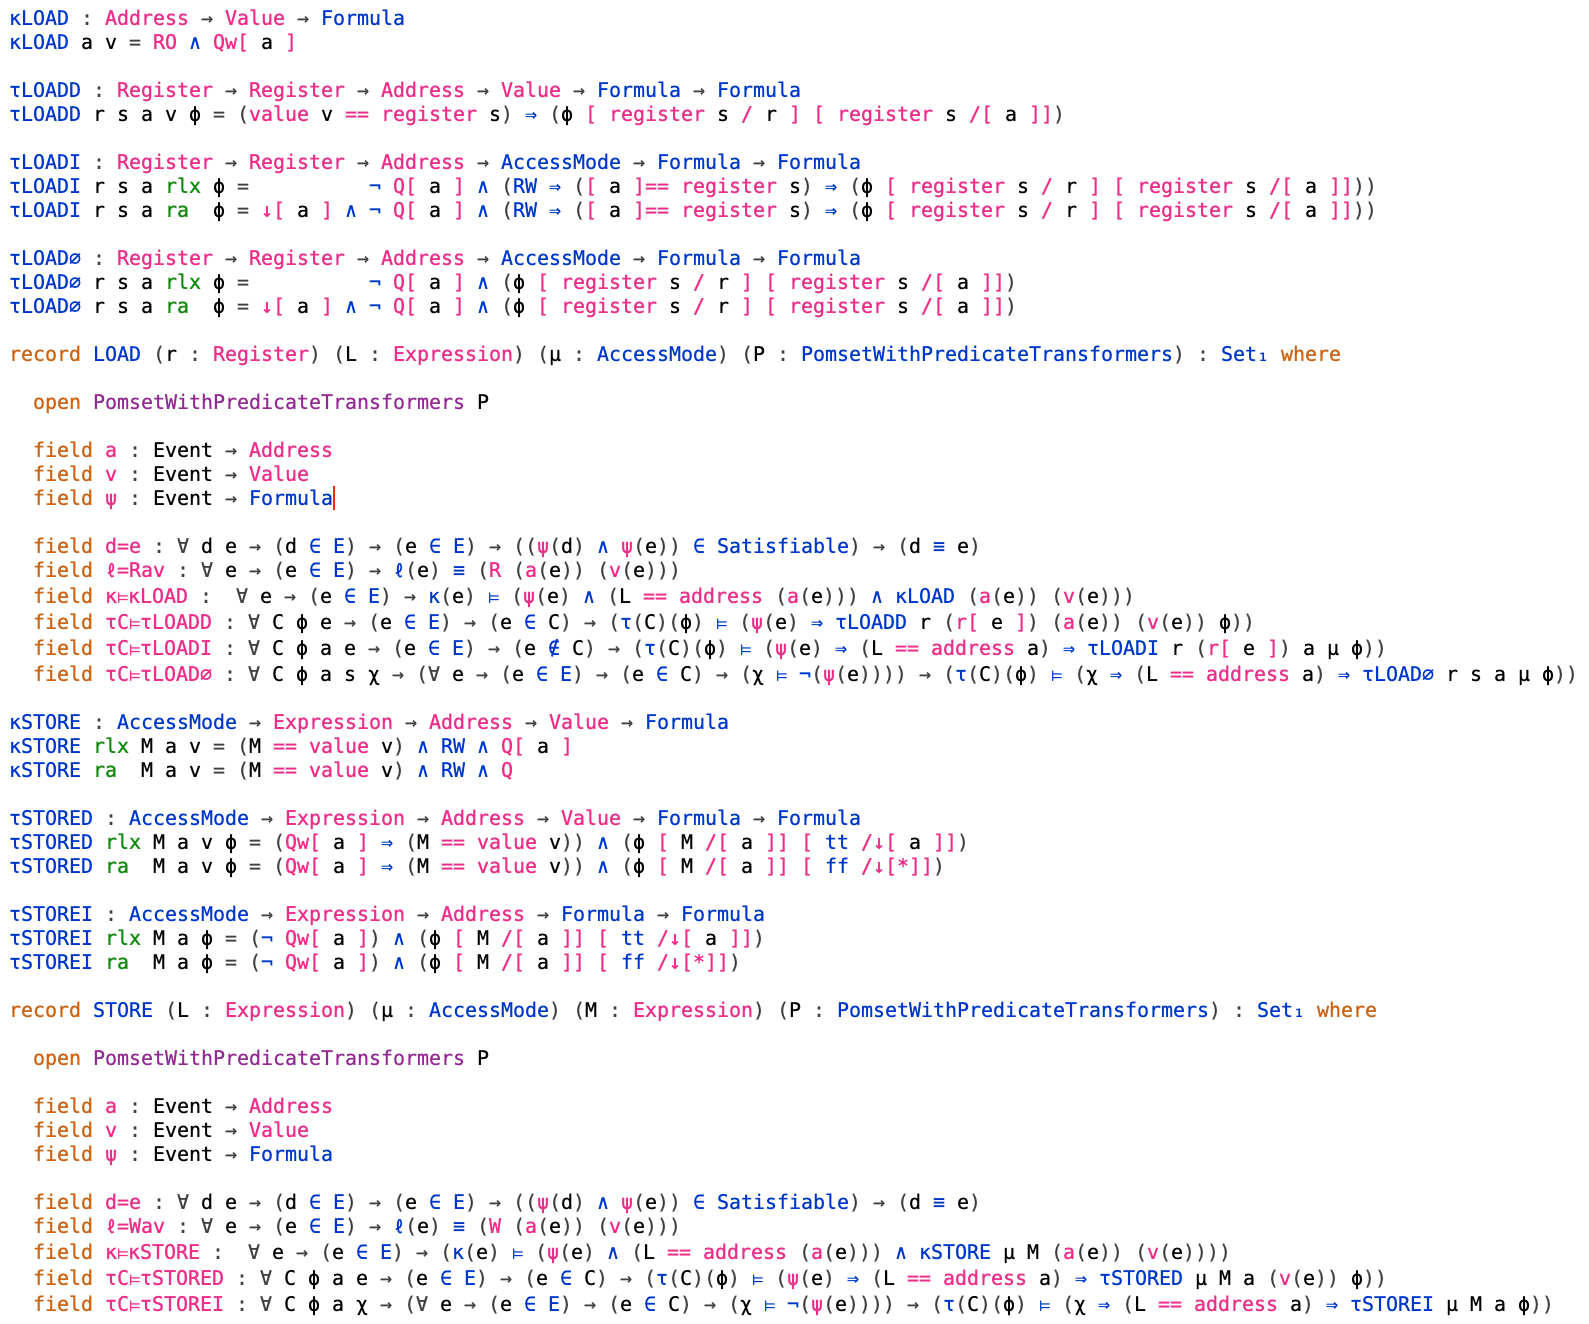
\includegraphics[width=\textwidth]{agda.png}
\end{figure*}

\section{Future Work}

\citet{DBLP:conf/esop/PaviottiCPWOB20} use step-indexing to account for
loops; we expect that the same approach could be applied here.

% We have presented the first model of relaxed memory that treats sequential
% composition as a first-class citizen. The model builds directly on \jjr{}.

% For sequential composition, parallel composition and the conditional, we
% believe that the definition is \emph{natural}, even \emph{canonical}.
% For stores and loads, instead, the definition in \reffig{fig:no-addr} is a
% Frankenstein's monster of features.  This complexity is \emph{essential},
% however, not just an accident of our poor choices.  Relaxed memory models must
% please many audiences: compiler writers want one thing, hardware designers
% another, and programmers yet another still.  The result is inevitably full of
% compromise.

% Given that \emph{complexity} cannot be eliminated from relaxed memory models,
% the best one can do is attempt to understand its causes.  We have broken the
% problem into seven manageable pieces, discussed throughout
% \textsection\ref{sec:q}--\ref{sec:complications}.  \refdef{def:pomsets-arm}
% summarizes all the features necessary for efficient implementation on
% \armeight{}.  We discuss address calculation, read-modify-write operations
% and fences in the appendix.

% {Logic} is the thread that sews these features together.

% %A unique feature of our model is the centrality of logic: 

% % study each feature in isolation, as a small delta to the base definition
% % given in \textsection\ref{sec:model}.
% % In we studied eight such
% % features.


% % seem staggeringly complex, we argue that this complexity is unavoidable if
% % one wants all the features that it embodies.  By breaking the definition into
% % its constituent parts, we have shown how each of eight


% \subsection*{Acknowledgements}
% % This paper has been greatly improved by the comments of the anonymous reviewers.
% Riely was supported by the National Science Foundation under
% grant No.~CCR-1617175.

% % It is based upon work supported by the National Science Foundation under
% % Grant No. CCR-1617175. Any opinions, findings, and conclusions or
% % recommendations expressed in this material are those of the author and do
% % not necessarily reflect the views of the NSF.}


\bibliography{bib}
\appendix
\section{Discussion}

\subsection{Relation to Traditional Predicate Transformers}

\begin{proposition}
  If $\aPS\in\sem{\aCmd}$ is top-level and quiescent then 
  $\aTr{\aEvs}{\bForm}$ implies $\fwp{\aCmd}{\bForm}$.

  For any substitution $\aSub=[{v_1/r_1},\ldots, {v_n/r_n}]$ there is some
  $\aPS\in\sem{\aCmd}$ %that is top-level and quiescent
  such that all preconditions in $\aPS\aSub$ are tautologies then 
  $\fwp{\aCmd}{\bForm}\aSub$
\end{proposition}

For a language where all programs are
terminating, we have for any statement $\aCmd$:
\begin{align*}
  \hoare{\aForm}{\aCmd}{\bForm} 
  \;\;\Leftrightarrow\;\;
  \aForm \textimplies \fwp{\aCmd}{\bForm}
\end{align*}
Interpretation is that if $\aState\models\fwp{\aCmd}{\bForm}$ and
$(\aState,\aCmd)\Downarrow\bState$
then $\bState\models\bForm$.

Let $\aCmd_0$ be
\begin{math}
  \PW{\aLoc_1}{\aVal_1}\SEMI\cdots\SEMI \PW{\aLoc_n}{\aVal_n}, 
\end{math}
such that $\fwp{\aCmd_0}{\aForm}$ is a tautology, and $\aLoc_i=\aLoc_j$
implies $i=j$.

Let $\aSub_\aPS=[{\aVal_1/\aLoc_1},\ldots, {\aVal_n/\aLoc_n}]$ be the final
state of $\aPS$.


For example, let $\aCmd_1=\PR{x}{r}$ and $\aCmd_2=\PW{x}{r{+}1}$ and
$\aCmd=\aCmd_1\SEMI \aCmd_2$.
\begin{align*}
  \fwp{\aCmd_2}{x{>}1}&=(r{+}1{>}1) = (r{>}0)
  \\
  \fwp{\aCmd_1}{r{>}0}=\fwp{\aCmd_0}{x{>}1}&=(x{>}0)
\end{align*}
Let $\aPS_i\in\sem{\aCmd_i}$.
\begin{align*}
  \aTr[2]{\aEvs_2}{x{>}1}&=(r{+}1{>}1) = (r{>}0)
  \\
  \aTr[0]{\aEvs_0}{x{>}1}&=(0{=}\aReg \limplies r{>}0)
  \\
  \aTr[0]{\aEvs_0}{x{>}1}&=(1{=}\aReg \limplies r{>}0)
  \\
  \aTr[0]{\aEvs_0}{x{>}1}&=(2{=}\aReg \limplies r{>}0)
\end{align*}

\begin{proposition}
  If $\aPS\in\sem{\aCmd}$ is top-level and quiescent then 
  $\aTr{\aEvs}{\aForm}$ implies $\fwp{\aCmd}{\aForm}$.

  For any substitution $\aSub=[{\aVal_1/\aReg_1},\ldots, {\aVal_n/\aReg_n}]$ there is some
  $\aPS\in\sem{\aCmd}$ %that is top-level and quiescent
  such that all preconditions in $\aPS\aSub$ are tautologies then 
  $\fwp{\aCmd}{\aForm}\aSub$
\end{proposition}

\subsection{[r/x] v [x/r]}

\begin{gather*}
  \PR{x}{s}\SEMI
  \IF{r\land s\;\mathsf{even}}\THEN \PW{y}{1}\FI\SEMI
  \IF{r\land s}\THEN \PW{z}{1}\FI
  \\
  \hbox{\begin{tikzinline}[node distance=0.5em and 1.5em]
      \event{a2}{\DR{x}{2}}{}
      \event{a3}{(x{=}s\lor2{=}s)\limplies (r\land s\;\mathsf{even})\mid\DW{y}{1}}{right=of a2}
      \event{a4}{(x{=}s\lor2{=}s)\limplies (r\land s)\mid\DW{z}{1}}{below=of a3}
    \end{tikzinline}}
\end{gather*}
Without substitution:
\begin{gather*}
  \PR{x}{r}\SEMI
  \PR{x}{s}\SEMI
  \IF{r\land s\;\mathsf{even}}\THEN \PW{y}{1}\FI\SEMI
  \IF{r\land s}\THEN \PW{z}{1}\FI
  \\
  \hbox{\begin{tikzinline}[node distance=0.5em and 1.5em]
      \event{a1}{\DR{x}{1}}{}
      \event{a2}{\DR{x}{2}}{below=of a1}
      \event{a3}{1{=}r\limplies  (x{=}s\lor2{=}s)\limplies (r\land s\;\mathsf{even})\mid\DW{y}{1}}{right=of a1}
      \event{a4}{1{=}r\limplies  (x{=}s\lor2{=}s)\limplies (r\land s)\mid\DW{z}{1}}{below=of a3}
      \po{a1}{a3}
      \po[out=-20,in=177]{a1}{a4}
    \end{tikzinline}}
\end{gather*}
Prepending $\PW{x}{0}$
\begin{gather*}
  % \PW{x}{0}\SEMI
  % \PR{x}{r}\SEMI
  % \PR{x}{s}\SEMI
  % \IF{r\land s\;\mathsf{even}}\THEN \PW{y}{1}\FI\SEMI
  % \IF{r\land s}\THEN \PW{z}{1}\FI
  % \\
  \hbox{\begin{tikzinline}[node distance=1.5em]
      \event{a0}{\DW{x}{0}}{}
      \event{a1}{\DR{x}{1}}{right=of a0}
      \event{a2}{\DR{x}{2}}{right=of a1}
      \event{a3}{\DW{y}{1}}{right=of a2}
      \event{a4}{\DW{z}{1}}{right=of a3}
      % \wk{a0}{a1}
      % \wk[out=-20,in=-160]{a0}{a2}
      \po[out=20,in=160]{a1}{a3}
      \po[out=20,in=160]{a1}{a4}
      \po[out=-20,in=-160]{a2}{a4}
    \end{tikzinline}}
\end{gather*}
With the substitution $[r/x]$:
\begin{gather*}
  \PR{x}{r}\SEMI
  \PR{x}{s}\SEMI
  \IF{r\land s\;\mathsf{even}}\THEN \PW{y}{1}\FI\SEMI
  \IF{r\land s}\THEN \PW{z}{1}\FI
  \\
  \hbox{\begin{tikzinline}[node distance=0.5em and 1.5em]
      \event{a1}{\DR{x}{1}}{}
      \event{a2}{\DR{x}{2}}{below=of a1}
      \event{a3}{1{=}r\limplies  (r{=}s\lor2{=}s)\limplies (r\land s\;\mathsf{even})\mid\DW{y}{1}}{right=of a1}
      \event{a4}{1{=}r\limplies  (r{=}s\lor2{=}s)\limplies (r\land s)\mid\DW{z}{1}}{below=of a3}
      \po{a1}{a3}
      \po[out=-20,in=177]{a1}{a4}
    \end{tikzinline}}
\end{gather*}
Prepending $\PW{x}{0}$
\begin{gather*}
  % \PW{x}{0}\SEMI
  % \PR{x}{r}\SEMI
  % \PR{x}{s}\SEMI
  % \IF{r\land s\;\mathsf{even}}\THEN \PW{y}{1}\FI\SEMI
  % \IF{r\land s}\THEN \PW{z}{1}\FI
  % \\
  \hbox{\begin{tikzinline}[node distance=1.5em]
      \event{a0}{\DW{x}{0}}{}
      \event{a1}{\DR{x}{1}}{right=of a0}
      \event{a2}{\DR{x}{2}}{right=of a1}
      \event{a3}{\DW{y}{1}}{right=of a2}
      \event{a4}{\DW{z}{1}}{right=of a3}
      % \wk{a0}{a1}
      % \wk[out=-20,in=-160]{a0}{a2}
      \po[out=20,in=160]{a1}{a3}
      \po[out=20,in=160]{a1}{a4}
      \po{a2}{a3}
    \end{tikzinline}}
\end{gather*}


\begin{comment}
  if in L6 we said [x/r], that says we know read the local version...  ignoring
  the value read...  Perhaps there is some intervening stuff that stops you
  from seeing the local state, such as release-acquire

  We could potentially get rid of [x/r] If you do two reads, your not allowed
  to be independent of the second based on the value that was read in the first
  read.

  x=0; r=x; if (r=1) { s=x; if (s=?) {y=1}}
  read 1 then 2.


  In order for the write to be independent of second read what does its
  precondition have to be.
  [r/x] then s==1
  no sub then s==0

  (s=? | Wy1)

  if (phi) z=1
  phi = s is even
  phi = s < 2

  With substitution you are saying you know that the ``local copy'' of x is the
  same as r.  Sitting in the local cache.  Read might have gone to main
  memory, but if it did it has updated the cache line so that the local copy is
  what I just read.

  If second read is a cache hit, then I know that I am seeing the same value.

  If we take substitution out then 
\end{comment}


\subsection{Fork-Join}

It is also possible to put coherence in the independency relation, in which
case, the semantics of $;$ includes the following.
\begin{enumerate}
  \setcounter{enumi}{\value{pomsetXSemiCount}}
\item
  \label{seq-reorder} if $\bEv\in\aEvs_1$ and $\aEv\in\aEvs_2$ either $\bEv<\aEv$ or $a\reorder\labeling_2(\aEv)$.
\end{enumerate}
One must be careful, however, due to \emph{inconsistency}.
Consider that \texttt{x=0;x=1} should not have completed pomset with only $\DWP{x}{0}$.

\eqref{seq-reorder} does not do the right thing with fork either.  If you
want to enforce coherence this way then you need to use fork-join as the
sequential combinator, rather than fork.


[We drop $\reorder$ because incompatible with $\sFORK{}$.  If you want to use
$\reorder$, then you need to use fork-join as the sequential combinator,
rather than fork.]

\begin{definition}
  A \emph{pomset with preconditions and termination} is
  a pomset with preconditions together with a predicate $\TICK$.
\end{definition}

% Define $\sTHREAD{}$ to transform a pomset with predicate transformers into a
% pomset with preconditions and termination by dropping the predicate
% transformer and setting $\TICK$ to indicate whether the pomset was completed.

% Extend the definition of $\sNIL$ so that $\TICK$ is true.

% Extend the definition of $\sPAR$ to handle for $\TICK$ by adding the
% following.
% \begin{enumerate}
%   \setcounter{enumi}{\value{pomsetPreParCount}}
% \item \label{par-tick}
%   if $\TICK$ then $\TICK_1$ and $\TICK_2$.
% \end{enumerate}

% Similarly, $\sFORKJOIN{}$ extends $\sFORK{}$ by adding the following.
% % \noindent
% % If $\aPS \in \sFORKJOIN{\aPSS}$ then
% % $(\exists\aPS_1\in\aPSS)$
% \begin{enumerate}
%   \setcounter{enumi}{\value{pomsetXForkCount}}
% \item $\TICK_1$.
% \end{enumerate}

\begin{definition}$\phantom{\;}$\par
  % \noindent
  % If $\aPS\in\sNIL$ then $\aEvs = \emptyset$ and $\TICK$.

  \noindent
  If $\aPS \in (\aPSS_1\sPAR\aPSS_2)$ then
  $(\exists\aPS_1\in\aPSS_1)$ $(\exists\aPS_2\in\aPSS_2)$
  \begin{enumerate}
    \setcounter{enumi}{\value{pomsetPreParCount}}
  \item[\ref{par-E}--\ref{par-kappa2})]
    as for $\sPAR$ in Definition~\ref{def:pomsets-pre},
  \item \label{par-tick}
    $\TICK$ implies $\TICK_1\land\TICK_2$.
  \end{enumerate}

  \noindent
  If $\aPS \in \sTHREAD{\aPSS}$ then
  $(\exists\aPS_1\in\aPSS)$
  \begin{enumerate}
    \setcounter{enumi}{\value{pomsetXThreadCount}}
  \item[\ref{thread-E}--\ref{thread-kappa})]
    as for $\sTHREAD{}$ in Definition~\ref{def:thread},
  \item if $\TICK$ then $\aTr{\aEvs}{\Q{}}$ implies $\Q{}$.
  \end{enumerate}    

  \noindent
  If $\aPS \in \sFORKJOIN{\aPSS}$ then
  $(\exists\aPS_1\in\aPSS)$
  \begin{enumerate}
    \setcounter{enumi}{\value{pomsetXForkCount}}
  \item[\ref{F1x}--\ref{F4x})]
    as for $\sFORK{}$ in Definition~\ref{def:fork},
  \item[{\labeltext[F5]{F5)}{F5}}]
    $\TICK_1$.
  \end{enumerate}    
\end{definition}

\begin{align*}
  \sem{\FORKJOIN{\aGrp}} &= \sFORKJOIN{}\sem{\aGrp}  
\end{align*}

We can then encode coherence as follows.
\begin{enumerate}
  \setcounter{enumi}{\value{pomsetXSemiCount}}
\item if $\bEv\in\aEvs_1$ and $\aEv\in\aEvs_2$ either $\bEv<\aEv$ or $a\reorder\labeling_2(\aEv)$.
\end{enumerate}


Access modes can be encoded in the independency relation, indexing labels by
$\amode$, but the extra flexibility of the logic is necessary for \armeight{}
(see \textsection\ref{sec:internal}).  Using independency, one would also
need another way to define completed pomsets.  Finally, this use of
independency is incompatible with fork (see \textsection\ref{sec:co}).


If we move coherence to independency (and use fork-join), we have the
following, assuming that each register occurs at most once.
\begin{align*}
  \QS{}{\mSC}&=\Q{\mSC}
  &\QS{}{\mRA}&=\Q{\mRA}
  &\QS{}{\mRLX}&=\Qx{\aLoc}
  \\
  \QL{}{\mSC}&=\Q{\mSC}
  &\QL{}{\mRA}&=\Qw{\aLoc}
  &\QL{}{\mRLX}&=\Qw{\aLoc}
  \\
  \DS{\aLoc}{\mSC}{\bForm}&=\bForm[\FALSE/\D]
  &\DS{\aLoc}{\mRA}{\bForm}&=\bForm[\FALSE/\D]
  &\DS{\aLoc}{\mRLX}{\bForm}&=\bForm[\TRUE/\Dx{\aLoc}] 
  \\
  \DL{\aLoc}{\mSC}&=\Dx{\aLoc}
  &\DL{\aLoc}{\mRA}&=\Dx{\aLoc}
  &\DL{\aLoc}{\mRLX}&=\TRUE
\end{align*}

% $\QS{}{\mRLX}=\TRUE$ and otherwise $\QS{}{\amode}=\Q{\amode}$.

% $\QL{}{\mSC}=\Q{\mSC}$ and otherwise $\QL{}{\amode}=\TRUE$.

% $\DS{\aLoc}{\mRLX}{\bForm}=\bForm[\TRUE/\Dx{\aLoc}]$ and otherwise
% $\DS{\aLoc}{\amode}{\bForm}=\bForm[\FALSE/\D]$. 

% $\DL{\aLoc}{\mRLX}=\TRUE$ and otherwise $\DL{\aLoc}{\amode}=\Dx{\aLoc}$.

% \begin{definition}$\phantom{\;}$\par
%   $\QS{}{\mRLX}=\TRUE$ and otherwise $\QS{}{\amode}=\Q{\amode}$.

%   $\QL{}{\mSC}=\Q{\mSC}$ and otherwise $\QL{}{\amode}=\TRUE$.

  \noindent
  If $\aPS \in \sSTORE[\amode]{\aLoc}{\aExp}$ then
  \begin{enumerate}
  \item[\ref{S1}--\ref{S2})] as before,
  \item[\ref{S3})]
    $\labelingForm(\aEv)$ implies
    \begin{math}
      \aExp{=}\aVal
      \land \RW
      \land \QS{}{\amode}
    \end{math},
  \item[\ref{S4})]
    $\aTr{\bEvs}{\bForm}$ implies 
    \begin{math}
      \aExp{=}\aVal
      \land \DS{\aLoc}{\amode}{\bForm[\aExp/{\aLoc}]}
    \end{math},
  \item[\ref{S5})]
    $\aTr{\emptyset}{\bForm}$ implies 
    \begin{math}
      \lnot\Q{\mRA}
      \land \DS{\aLoc}{\amode}{\bForm[\aExp/{\aLoc}]}
    \end{math}
  \end{enumerate}

  \noindent
  If $\aPS \in \sLOAD[\amode]{\aReg}{\aLoc}$ then
  \begin{enumerate}
  \item[\ref{L1}--\ref{L2})] as before,
  \item[\ref{L3})] $\labelingForm(\aEv)$ implies
    \begin{math}
      \RO
      \land \QL{}{\amode}
    \end{math},
  \item[\ref{L4})]
    $\aTr{\bEvs}{\bForm}$ implies
    \begin{math}
      (\aVal{=}\aReg)
      \limplies \bForm[\aReg/{\aLoc}]
    \end{math}
  \item[\ref{L5})] 
    $\aTr{\emptyset}{\bForm}$ implies
    \begin{math}
      \DL{\aLoc}{\amode}
      \land \lnot\Q{\mRA}
      \land
      (\RW
      \limplies (\aVal{=}\aReg\lor\aLoc{=}\aReg) 
      \limplies \bForm[\aReg/{\aLoc}]
      ).
    \end{math}
  \end{enumerate}  



\subsection{Must Allow Inconsistent Preconditions}

Removing the requirements for
\emph{consistency} and \emph{causal strengthening}, and

[The definition does not give a sensible notion of completed execution
without consistency and causal strengthening.]

%Item \ref{pre-reorder} does not impose coherence.
  

\subsection{Skolemization}

\jjr{} is non-skolemized, using substitution instead, and collapsing $\aLoc$
and $\aReg$.
There, item \ref{loadpre-kappa2}  of $\sLOADPRE{}{}{}$ is written 
\begin{enumerate}
\item[] %[\ref{loadpre-kappa2})]
  if $\aEv\in\aEvs_2\setminus\aEvs_1$ then either \\
  $\labelingForm(\aEv)$ implies $\labelingForm_2(\aEv)[\aLoc/\aReg][\aVal/\aLoc]$ and $(\exists\bEv\in\aEvs_1)\bEv{<}\aEv$, or \\
  $\labelingForm(\aEv)$ implies
  $\labelingForm_2(\aEv)[\aLoc/\aReg][\aVal/\aLoc] \land \labelingForm_2(\aEv)[\aLoc/\aReg]$.
\end{enumerate}


\jjr{} is non-skolemized---with $[x/r]$ rather than no substitution.
\begin{enumerate}
\item[\ref{L4})]
  $\aTr{\bEvs}{\bForm}$ implies $\bForm[\aLoc/\aReg][\aVal/\aLoc]$, 
\item[\ref{L5})]
  $\aTr{\emptyset}{\bForm}\;$ implies $\bForm[\aLoc/\aReg][\aVal/\aLoc]\land\bForm[\aLoc/\aReg]$,
\item[\ref{L6})]
  $\aTr{\emptyset}{\bForm}\;$ implies $\bForm[\aLoc/\aReg]$.
\end{enumerate}

[Skolemization ensures disjunction closure, which is necessary
for associativity. Show example.]

\subsection{Reads Update Local State}
 In the rule for read prefixing we have substituted $[r/x]$, rather than
$[x/r]$.  This means that reads clobber local state.  We assume registers are
only used once---otherwise, one needs to generate a fresh register for the
substitution.

With read-read dependencies, this difference can be seen.  For example, the
following execution is allowed with $[x/r]$, but not $[r/x]$.
\begin{gather*}
  \PW{x}{0}\SEMI
  \PR{x}{r}\SEMI
  \IF{r}\THEN \PR{x}{s}\FI\SEMI
  \PW{y}{s{+}1}
  \PAR
  \PW{x}{\PR{y}{}}
  \\[-1ex]
  \hbox{\begin{tikzinline}[node distance=1.5em]
      \event{a1}{\DW{x}{0}}{}
      \event{a2}{\DW{x}{1}}{right=of a1}
      \event{a3}{\DR{x}{0}}{right=of a2}
      \event{a4}{\DW{y}{1}}{right=of a3}
      \event{b1}{\DR{y}{1}}{right=3em of a4}
      \event{b2}{\DW{x}{1}}{right=of b1}
      \wk{a1}{a2}
      \po{a2}{a3}
      \po{b1}{b2}
      \rf{a4}{b1}
      \rf[out=165,in=15]{b2}{a2}
    \end{tikzinline}}
\end{gather*}
[Is there a difference w/o read-read dependencies?]

[Don't need extended expressions anymore, since never substituting with $x$
for anything.]



\subsection{Parallel Composition}

In \jjr{\textsection2.4}, parallel composition is defined allowing coalescing
of events.  Here we have forbidden coalescing.  This difference appears to be
arbitrary.  In \jjr{}, however, there is a mistake in the handling of
termination actions.  The predicates should be joined using $\land$, not
$\lor$.

\subsection{Redundant Read Elimination}

Requires indexing to resolve nondeterminism.

\begin{gather*}
  \taglabel{TC2}
  \PR{x}{r}\SEMI
  \PR{x}{s}\SEMI
  \IF{r{=}s}\THEN \PW{y}{1}\FI
  \PAR
  x\GETS y
  \\
  \hbox{\begin{tikzinline}[node distance=1.5em]
      \event{a1}{\DR{x}{1}}{}
      \event{a2}{\DR{x}{1}}{right=of a1}
      \event{a3}{\DW{y}{1}}{right=of a2}
      % \po{a2}{a3}
      % \po[out=-20,in=-160]{a1}{a3}
      \event{b1}{\DR{y}{1}}{right=3em of a3}
      \event{b2}{\DW{x}{1}}{right=of b1}
      \rf{a3}{b1}
      \po{b1}{b2}
      \rf[out=169,in=11]{b2}{a2}
      \rf[out=169,in=11]{b2}{a1}
    \end{tikzinline}}
\end{gather*}
Precondition of $\DWP{y}{1}$ is $(r{=}s)$ in
\begin{math}
  \sem{\IF{r{=}s}\THEN y\GETS 1\FI}.
\end{math}
Predicate transformers for $\emptyset$ in $\sem{\PR{x}{r}}$ and $\sem{\PR{x}{s}}$ are
\begin{align*}
  \PREDP{(r{=}1 \lor r{=}x)\limplies\bForm[r/x]},
  \\
  \PREDP{(s{=}1 \lor s{=}x)\limplies\bForm[s/x]}.
\end{align*}
Combining the transformers, we have
\begin{displaymath}
  \PREDP{(r{=}1 \lor r{=}x)\limplies(s{=}1 \lor s{=}r)\limplies\bForm[s/x]}.
\end{displaymath}
Applying this to $(r{=}s)$, we have
\begin{displaymath}
  \PREDP{(r{=}1 \lor r{=}x)\limplies (s{=}1 \lor s{=}r)\limplies (r{=}s)},
\end{displaymath}
which is not a tautology.

Same problem occurs \jjr{}, where we have:
\begin{align*}
  \PREDP{\bForm[v/x,r] \land \bForm[x/r]},
  \\
  \PREDP{\bForm[v/x,s] \land \bForm[x/s]}.
\end{align*}
Combining the transformers, we have
\begin{displaymath}
  \PREDP{\bForm[v/x,r,s] \land \bForm [v/x,r][x/s] \land \bForm[x/r][v/x,s] \land \bForm[x/r,s]}.
\end{displaymath}
Applying this to $(r{=}s)$, we have
\begin{displaymath}
  \PREDP{v{=}v \land v{=}x \land x{=}v \land x{=}x},
\end{displaymath}
which is not a tautology.

The semantics here allows this by coalescing:
\begin{gather*}
  r\GETS x\SEMI
  s\GETS x\SEMI
  \IF{r{=}s}\THEN y\GETS 1\FI
  \PAR
  x\GETS y
  \\
  \hbox{\begin{tikzinline}[node distance=1.5em]
      \event{a1}{\DR{x}{1}}{}
      \event{a3}{\DW{y}{1}}{right=of a1}
      \event{b1}{\DR{y}{1}}{right=3em of a3}
      \event{b2}{\DW{x}{1}}{right=of b1}
      \rf{a3}{b1}
      \po{b1}{b2}
      \rf[out=169,in=11]{b2}{a1}
    \end{tikzinline}}
\end{gather*}

\subsection{Redundant Read Elimination}

In \jjr{\textsection2.6} the semantics of read is defined as follows:
\begin{align*}
  \sem{\aReg\GETS\aLoc^\amode\SEMI \aCmd} & \eqdef \textstyle\bigcup_\aVal\;
  (\DRmode\aLoc\aVal) \prefix \sem{\aCmd} [\aLoc/\aReg]
\end{align*}
The definition of prefixing$((\aForm \mid \aAct) \prefix \aPSS)$ has several clauses.
The most relevant are as follows, where $\bEv$ is the new event labeled with
$(\aForm \mid \aAct)$ and $\aEv$ is an event from $\aPSS$:
\begin{description}
\item[{\labeltextsc[P4c]{(P4c)}{4c}}]
  If $\bEv$ reads $\aVal$ from $\aLoc$ then either $\aEv=\bEv$ or
  $\labelingForm'(\aEv)$ implies $\labelingForm(\aEv)[\aVal/\aLoc]$.
\item[{\labeltextsc[P5a]{(P5a)}{5a}}]\labeltextsc[P5]{}{5}%
  If $\bEv$ reads and $\aEv$ writes then either $\labelingForm'(\aEv)$
  implies $\labelingForm(\aEv)$ or $\bEv\le'\aEv$.
% \item[{\labeltextsc[P5b]{(P5b)}{5b}}]
%   If $\bEv$ and $\aEv$ are in conflict then $\bEv\le'\aEv$.
\end{description}

We have discovered two issues with this definition.

The first issue concerns the substitution $[\aLoc/\aReg]$.  It should be
$[\aReg/\aLoc]$.  We noticed this error while developing the alternative
characterization presented here.  The error causes redundant read elimination
to fail in \jjr{}.  As a result, common subexpression elimination also fails.
The problem can be seen in \ref{TC2}.
\begin{gather*}
  \taglabel{TC2}
  r\GETS x\SEMI
  s\GETS x\SEMI
  \IF{r{=}s}\THEN y\GETS 1\FI
  \PAR
  x\GETS y
\end{gather*}
% In \jjr{\textsection3.1},
We claimed that \ref{TC2} allowed the following
execution:
\begin{gather*}
  \hbox{\begin{tikzinline}[node distance=1.5em]
  \event{a1}{\DR{x}{1}}{}
  \event{a2}{\DR{x}{1}}{right=of a1}
  \event{a3}{\DW{y}{1}}{right=of a2}
  % \po{a2}{a3}
  % \po[out=15,in=165]{a1}{a3}
  \event{b1}{\DR{y}{1}}{right=3em of a3}
  \event{b2}{\DW{x}{1}}{right=of b1}
  \rf{a3}{b1}
  \po{b1}{b2}
  \rf[out=169,in=11]{b2}{a2}
  \rf[out=169,in=11]{b2}{a1}
    \end{tikzinline}}
\end{gather*}
But this execution is not possible using the semantics of \jjr{}:
$\DWP{y}{1}$ has precondition $r{=}s$ in
\begin{math}
  \sem{\IF{r{=}s}\THEN y\GETS 1\FI}.
\end{math}
Given the lack of order in the execution, the precondition of $\DWP{y}{1}$
must entail $r{=}1\land r{=}x$ in 
\begin{math}
  \sem{s\GETS x\SEMI
  \IF{r{=}s}\THEN y\GETS 1\FI}.
\end{math}
\ref{4c} imposes $r{=}1$, and \ref{5a} imposes $r{=}x$.  Adding the second
read, the precondition of $\DWP{y}{1}$ must entail both $1{=}1\land 1{=}x$
and also $x{=}1\land x{=}x$.  This can be simplified to $x{=}1$.  This leaves
a requirement that must be satisfied by a preceding write.  Since the
preceding write is the initialization to $0$, the requirement cannot be
satisfied, and the execution is impossible.\footnote{In \jjr{} we ignore the
  middle terms, mistakenly simplifying this to $1{=}1\land x{=}x$.
  Correcting the error, the attempted execution is:
\begin{gather*}
  \hbox{\begin{tikzinline}[node distance=1.5em]
  \event{a1}{\DR{x}{1}}{}
  \event{a2}{\DR{x}{1}}{right=of a1}
  \event{a3}{\DW{y}{1}}{right=of a2}
  \po{a2}{a3}
  \po[out=-20,in=-160]{a1}{a3}
  \event{b1}{\DR{y}{1}}{right=3em of a3}
  \event{b2}{\DW{x}{1}}{right=of b1}
  \rf{a3}{b1}
  \po{b1}{b2}
  \rf[out=169,in=11]{b2}{a2}
  \rf[out=169,in=11]{b2}{a1}
    \end{tikzinline}}
\end{gather*}}

The substitution $[\aLoc/\aReg]$ leaves the obligation on $\aLoc$ to be
fulfilled by the preceding write.  Thus, the read does not update the
\emph{value} of $\aLoc$ in subsequent predicates.  The substitution
$[\aReg/\aLoc]$, instead, does update the value of $\aLoc$, thus removing any
obligation on $\aLoc$ for preceding code.

In order to write this, we must update the definition of prefixing reads to
include the register.  Then \ref{4c} becomes:
\begin{description}
\item[\textsc{(p4c)}] If $\bEv$ reads $\aVal$ from $\aLoc$ then either
  $\aEv=\bEv$ or $\labelingForm'(\aEv)$ implies
  $\labelingForm(\aEv)[\aVal/\aReg]$.
\end{description}

We can then reason with \ref{TC2} as follows: $\DWP{y}{1}$ has precondition
$r{=}s$ in
\begin{math}
  \sem{\IF{r{=}s}\THEN y\GETS 1\FI}.
\end{math}
To avoid introducing order in the execution, the precondition of $\DWP{y}{1}$
must entail $r{=}1\land r{=}s$ in 
\begin{math}
  \sem{s\GETS x\SEMI
  \IF{r{=}s}\THEN y\GETS 1\FI}.
\end{math}
\ref{4c} imposes $r{=}1$, and \ref{5a} imposes $r{=}x$.  Adding the second
read, the precondition of $\DWP{y}{1}$ must entail both $1{=}1\land 1{=}x$
and also $x{=}1\land x{=}x$.  This can be simplified to $x{=}1$.  This leaves
a requirement that must be satisfied by a preceding write.


With read elimination, the rule for relaxed reads is as follows:
\begin{align*}
  \sem{\PR{\aLoc}{\aReg} \SEMI \aCmd} &\eqdef
  \sem{\aCmd}[\aLoc/\aReg]
  \cup
  \textstyle\bigcup_\aVal\;
  \DRP{\aLoc}{\aVal} \prefix_{\aReg} %\Rdis{\aLoc}{\aVal}
  \sem{\aCmd}[\aReg/\aLoc]
\end{align*}
It is interesting to note that the substitution is $[\aLoc/\aReg]$ on
eliminated reads, and $[\aReg/\aLoc]$ on non-eliminated reads.  Intuitively,
the subsequent value of $\aLoc$ is fixed by an explicit read, but not for an
eliminated read.  In the latter case, the value is fixed by some preceding
action.  The preceding action may itself be a read. This gives rise to some
fear that we might introduce thin-air reads, since we do not enforce
read-read coherence.  But this is not the case.  Consider the following example:
\begin{gather*}
  r\GETS x\SEMI
  s\GETS x\SEMI
  y\GETS s
  \PAR
  x\GETS y
  \\
  \hbox{\begin{tikzinline}[node distance=1.5em]
  \event{a1}{\DR{x}{1}}{}
  \event{a2}{\DR{x}{1}}{right=of a1}
  \event{a3}{\DW{y}{1}}{right=of a2}
  %\po{a2}{a3}
  \po[out=-20,in=-160]{a1}{a3}
  \event{b1}{\DR{y}{1}}{right=3em of a3}
  \event{b2}{\DW{x}{1}}{right=of b1}
  \rf{a3}{b1}
  \po{b1}{b2}
  \rf[out=169,in=11]{b2}{a2}
  \rf[out=169,in=11]{b2}{a1}
    \end{tikzinline}}
  \\
  \hbox{\begin{tikzinline}[node distance=1.5em]
  \event{a1}{\DR{x}{1}}{}
  \internal{a2}{\DR{x}{1}}{right=of a1}
  \event{a3}{\DW{y}{1}}{right=of a2}
  %\po{a2}{a3}
  \po[out=-20,in=-160]{a1}{a3}
  \event{b1}{\DR{y}{1}}{right=3em of a3}
  \event{b2}{\DW{x}{1}}{right=of b1}
  \rf{a3}{b1}
  \po{b1}{b2}
  %\rf[out=169,in=11]{b2}{a2}
  \rf[out=169,in=11]{b2}{a1}
    \end{tikzinline}}
\end{gather*}
But this is not a problem, since fulfillment requires that $\DWP{x}{1}$
precede both reads of $x$.

\subsection{Internal Acquiring Reads}

Our solution allows executions that are not allowed under \armeight{} since
we do not insist that the local relaxed write is actually read from.  This
may seem counterintuitive, but we don't see a local way to be more precise.


The second issue concerns acquiring reads.  Shortly after publication,
\citet{anton} noticed a shortcoming of the implementation on \armeight{} in
\jjr{\textsection 7}.  The proof given there assumes that all internal reads
can be dropped.  However, this is not the case for acquiring reds.  For
example, \jjr{} disallows the following execution, which is allowed by
\armeight{} and \tso{}.
\begin{gather*}
  \PW{x}{2}\SEMI 
  \PR[\mRA]{x}{r}\SEMI
  \PR{y}{s} \PAR
  \PW{y}{2}\SEMI
  \PW[\mRA]{x}{1}
  \\
  \hbox{\begin{tikzinline}[node distance=1.5em]
      \event{a}{\DW{x}{2}}{}
      \raevent{b}{\DR[\mRA]{x}{2}}{right=of a}
      \event{c}{\DR{y}{0}}{right=of b}
      \event{d}{\DW{y}{2}}{right=2.5em of c}
      \raevent{e}{\DW[\mRA]{x}{1}}{right=of d}
      \rf{a}{b}
      \sync{b}{c}
      \wk{c}{d}
      \sync{d}{e}
      \wk[out=-165,in=-15]{e}{a}
      % \rfi{a}{b}
      % \bob{b}{c}
      % \fre{c}{d}
      % \bob{d}{e}
      % \coe[out=-165,in=-15]{e}{a}
    \end{tikzinline}}
\end{gather*}
The solution we have adopted is to allow an acquiring read to be downgraded
to a relaxed read when it is preceded (sequentially) by a relaxed write that
could fulfill it.  Back-porting this solution to \jjr{} requires that we add
access predicates to the logic and allow

\subsection{Triangular Races}

The notion of data-race is incorrect in \jjr{}.
\begin{gather*}
  \PW{x}{1}\SEMI
  \PW[\mRA]{y}{1}\SEMI
  \PR[\mRA]{x}{r}
  \PAR
  \IF{\PR[\mRA]{y}{}}\THEN \PW[\mRA]{x}{2}\FI
  \\
  \hbox{\begin{tikzinline}[node distance=1.5em]
      \event{a1}{\DW{x}{1}}{}
      \raevent{a2}{\DW[\mRA]{y}{1}}{right=of a1}
      \raevent{a3}{\DR[\mRA]{x}{1}}{right=of a2}
      \raevent{b1}{\DR[\mRA]{y}{1}}{right=3em of a3}
      \raevent{b2}{\DW[\mRA]{x}{2}}{right=of b1}
      \sync{a1}{a2}
      \rf[out=20,in=160]{a1}{a3}
      \rf[out=20,in=160]{a2}{b1}
      \sync{b1}{b2}
    \end{tikzinline}}
  \\
  \hbox{\begin{tikzinline}[node distance=1.5em]
      \event{a1}{\DW{x}{1}}{}
      \raevent{a2}{\DW[\mRA]{y}{1}}{right=of a1}
      \raevent{a3}{\DR[\mRA]{x}{2}}{right=of a2}
      \raevent{b1}{\DR[\mRA]{y}{1}}{right=3em of a3}
      \raevent{b2}{\DW[\mRA]{x}{2}}{right=of b1}
      \sync{a1}{a2}
      \rf[out=20,in=160]{a2}{b1}
      \rf[out=160,in=20]{b2}{a3}
      \sync{b1}{b2}
    \end{tikzinline}}
\end{gather*}
Bug is in \citep[Lemma A.4]{DBLP:conf/ppopp/DongolJR19}.  It assumes that
$\DRP[\mRA]{x}{1}$ and $\DWP[\mRA]{x}{2}$ are racing in the first execution
because they are not ordered by happens-before.  But this is false since
neither is plain.

In addition, the \armeight{} implementation result given here does not rely
on read elimination.  Instead we use a recent alternative characterization of
\armeight{} \citep{alglave-git-alternate,arm-reference-manual,armed-cats}.


\end{document}

% Local Variables:
% mode: latex
% TeX-master: t
% End:
